\documentclass[a4paper]{report}
\usepackage[table]{xcolor}
\usepackage[top=3cm, bottom=3cm, left=4cm, right=4cm]{geometry}
\usepackage{graphicx}
\usepackage{svg}
\usepackage{lipsum}
\usepackage{amsmath}
\usepackage{amssymb}
\usepackage{mathtools}
\usepackage[parfill]{parskip}
\usepackage[font={small,it}]{caption}
\usepackage{enumitem}
\usepackage[hidelinks]{hyperref}
\usepackage{quoting}

% Biliography
\usepackage[sectionbib, numbers]{natbib}
\usepackage{chapterbib}

% Colors 
\definecolor{aux_pink}{HTML}{9F1F79}
\definecolor{aux_green}{HTML}{006561}

% Headers and footers
\usepackage{fancyhdr}
\pagestyle{fancy}
\fancyhead{}
\fancyhead[L]{\leftmark}
\fancyfoot{}
\fancyfoot[C]{\thepage}

% Example box
\usepackage{tcolorbox}
\tcbuselibrary{theorems, breakable}
\newtcbtheorem{example}{Example}%
{colback=gray!5,colframe=white!35!black,fonttitle=\bfseries, breakable}{ex}
\newtcbtheorem{objectives}{Learning objectives}%
{colback=aux_green!5,colframe=white!35!aux_green,fonttitle=\bfseries, breakable}{lo}

% Aliases and macros
\newcommand{\tr}[1]{{\mathrm{tr}}( #1 )}
\renewcommand{\arraystretch}{1.3}
\renewcommand{\abstractname}{General information}


\title{Structural Optimization}
\author{Nils Meyer}
\date{May 2023}

\begin{document}

\maketitle

\begin{abstract}
    This is the lecture manuscript for the course \emph{Structural optimization (MRM-0156)} held during the summer term 2023 at University of Augsburg. 

    Accompanying code to reproduce examples and figures may be found at \url{https://github.com/meyer-nils/structural_optimization}. This repository also stores solutions to the exercise tasks. Solving the exercises and examples on your own is vital to gather proper understanding of the presented topics. 

    Credits are assigned in an oral examination in combination with a semester task that has to be submitted prior to the examination. This task should demonstrate that you are capable to apply and extend methods of this course to a problem of your own choice. An example for a semester task would be an extension of the presented two-dimensional truss problems to three-dimensional problems. 

    This course is held for the first time in summer term 2023. Even though the manuscript was prepared with great care, it is likely that it still contains mistakes. If you find one or if you are in doubt, please don't hesitate to contact \href{mailto:nils.meyer@uni-a.de}{nils.meyer@uni-a.de}. 
\end{abstract}

\setcounter{tocdepth}{1}
\tableofcontents

\chapter{Introduction}
The first chapter introduces the basic terms for structural optimization. In addition, it introduces the mathematical notation used throughout this lecture and repeats some basic concepts of tensor algebra and tensor analysis. 

\begin{objectives}{}{objectives_introduction}
After studying this chapter and finishing the exercise, you should be able to 
\begin{itemize}[label=$\dots$]
    \item distinguish three types of structural optimization problems.
    \item perform tensor algebra computations such as inner products, cross products, and outer products.
    \item employ index notation confidently.
    \item apply differential operators such as divergence and gradient on tensor fields.
\end{itemize}
\end{objectives}


\section{What is structural optimization?}
Following Gordon \cite{Gordon2003}, a \emph{structure} is "any assemblage of materials which is intended to sustain loads". The term \emph{optimization} means making things best. Thus, \emph{structural optimization} is the subject of making an assemblage of materials sustain loads in the best way \cite{Christensen2008}. 

The term \emph{best} depends on what we define to be the \emph{objective function} of our design problem. It could be the weight to obtain light structures, it could be the cost to obtain cheap structures, or it could be CO\textsubscript{2} emissions to obtain sustainable structures. Usually the optimization is subject to some \emph{constraints}, for example a certain load that has to be endured without permanent deformation. The variables that we can change to optimize the objective function are called \emph{design variables}. Depending on the choice of design variables, we generally divide three types of structural optimization problems: 
\begin{description}
    \item[Sizing optimization]{The design variables describe some technical parameters of a structure, e.g. wall thickness, diameters of holes, or the cross section of beams. We seek the optimal size of these parameters in he optimization task.}
    \item[Shape optimization]{The design variables describe the contour or boundary of a part. We seek the optimal shape of the part boundaries in the optimization task.}
    \item[Topology optimization]{The design variables describe the presence of material in a design space. We seek the optimal distribution of material within that design space.}
\end{description}

\begin{figure}[!htpb]
    \centering
    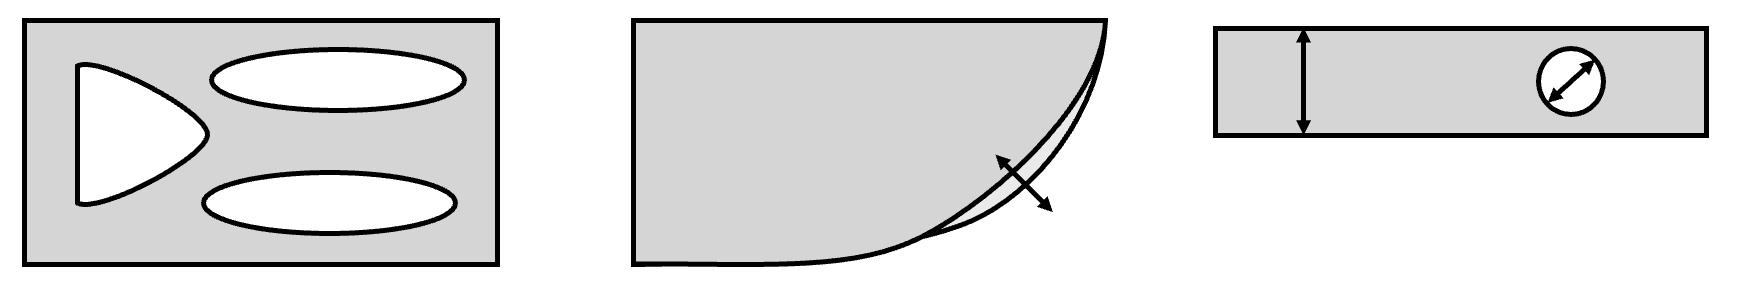
\includegraphics[width=\textwidth]{figures/structural_optimization_types.png}
    \caption{Types of structural optimization (left to right): Topology optimization, shape optimization, sizing optimization.}
    \label{fig:structural_optimization_types.}
\end{figure}

Before we can start optimizing structures, we need to recapitulate some basic tensor math, continuum mechanics and fundamentals of optimization, though. 

\section{Tensor algebra}
During this lecture we will deal with spaces, scalars, vectors, tensors, matrices and other mathematical objects. To support understanding of which objects are used in each context, we introduce some notation rules. 

\subsection{Scalars}
A scalar variable, such as a temperature, has no direction and is completely described by a single real value. Scalars are denoted as variables in regular font, for example
\begin{equation}
    a \in \mathcal{R}.
\end{equation}

\subsection{Vectors}
Most objects have some sort of direction associated to it (e.g. a velocity or a force). They are defined in a \emph{vector space} 
$\mathcal{R}^d$, where $d$ is the dimension of the vector space. A \emph{vector} is an element of the vector space that fulfills so-called vector axioms and is denoted with lowercase letters in bold font, e.g. 
\begin{equation}
    \textbf{a} \in \mathcal{R}^d.
\end{equation}
In order to describe components of a vector, it is convenient to define a \emph{basis}. A basis is given by a subset of vectors ${\mathbf{e}_1,\mathbf{e}_2,...,\mathbf{e}_d}$ that are linearly independent and span the entire vector space.
More specifically, we use an orthonormal basis (\emph{ONB}) that is spanned by normalized and orthogonal vectors $\{\mathbf{e}_i\}$. The orthogonality is expressed as  
\begin{equation}
    \label{eq:orthogonality}
    \mathbf{e}_i \cdot \mathbf{e}_j = \delta_{ij}
\end{equation}
with the \emph{Kronecker symbol} 
\begin{equation}
    \delta_{ij} = 
    \begin{cases}
    1 & \text{if }  i=j \\
    0 & \text{else}.
    \end{cases}
\end{equation}

\begin{example}{Standard basis in 3D Euclidean space}{basis_example}
    The standard basis for the three-dimensional ($d=3$) Euclidean space is given by the set of three vectors
    \begin{equation}
        \{\mathbf{e}_1=(1,0,0), \mathbf{e}_2=(0,1,0), \mathbf{e}_3=(0,0,1)\}.
    \end{equation}
\end{example}

With a basis, we can define a vector in terms of \emph{coordinates} $(a_1, a_2, ..., a_d)$ as 
\begin{equation}
    \label{eq:coordinates}
    \mathbf{a} = \sum_i a_i \mathbf{e}_i. 
\end{equation}
It is important to note that these coordinates depend on the basis. The same vector $\mathbf{a}$ may be expressed with coordinates $(a_1, a_2, ..., a_d)$ for a basis $\{\mathbf{e}_i\}$ and $(\tilde{a}_1, \tilde{a}_2, ..., \tilde{a}_d)$ for a basis $\{\tilde{\mathbf{e}}_i\}$. 

%It is a bit cumbersome to write the summation sign all the time. Therefore, we apply \emph{Einstein's summation convention} or \emph{index notation}: We omit the summation sign, but keep in mind that if two equal indices appear in an expression, then we sum over that index. Therefore the expressions
%\begin{equation}
%    \mathbf{a} \Leftrightarrow \sum_i a_i \mathbf{e}_i \Leftrightarrow a_i \mathbf{e}_i \Leftrightarrow a_i
%\end{equation}
%are equivalent, where the last expression $a_i$ omitted the basis assuming that it is the standard basis.

We define the \emph{inner product} or \emph{scalar product} of two vectors $\mathbf{a}, \mathbf{b} \in \mathcal{R}^d \rightarrow \mathcal{R}$ as 
\begin{equation}
    \mathbf{a} \cdot \mathbf{b} 
        = \sum_i a_i \mathbf{e}_i \cdot \sum_j b_j \mathbf{e}_j 
        =  \sum_{i,j} a_i b_j \overbracket{(\mathbf{e}_i \cdot \mathbf{e}_j)}^{\delta_{ij}} 
        = \sum_{i,j} a_i b_j \delta_{ij} = \sum_{i} a_i b_i
\end{equation}
using Equation \eqref{eq:orthogonality}.
There are two remarks at this point: First, the result of the scalar product between two vectors is a scalar as it is just a summation of coordinates. Second, the Kronecker symbol can be interpreted as an operator that replaces an index.

\begin{example}{Calculations with the Kronecker symbol}{kronecker}
    These are a couple of examples for Kronecker computations: 
    \begin{align}
        \delta_{11}     &= 1\\
        a \delta_{33}   &= a \\
        \sum_i \delta_{ii} &= d 
    \end{align}
\end{example}

The cross product between two vectors results in a vector perpendicular to the first two vectors and a magnitude equal to the area spanned by the two vectors. It can be denoted for two vectors $\mathbf{a},\mathbf{b} \in \mathcal{R}^3 \rightarrow \mathcal{R}^3$ as 
\begin{equation}
    \mathbf{a} \times \mathbf{b} = \sum_i \epsilon_{ijk} a_j b_k \mathbf{e}_i 
\end{equation}
with the permutation symbol 
\begin{equation}
    \epsilon_{ijk} = 
    \begin{cases}
        +1  & \text{if } (ijk) \text{ is an even permutation of } (1,2,3)\\
        -1  & \text{if } (ijk) \text{ is an odd permutation of } (1,2,3)\\
        0   & \text{else}.
    \end{cases}
\end{equation}

\subsection{Tensors}
Vectors are not sufficient to describe all directional objects needed in this lecture. A stress, for example, results in a traction vector that also depends on the cutting plane defined by its normal direction. 
% following the Lemma of Cauchy 
% \begin{equation}
%     \mathbf{t} = \pmb{\sigma} \mathbf{n} = \sigma_{ij} n_j \mathbf{e}_i.
% \end{equation}
In a sense, the stress tensor combines two directions and we learn in basic mechanics courses that one index is attributed to the direction and one to the plane. We can also think about the stress tensor as a mapping from one vector to another vector or as a multi-dimensional array containing the values of $S_{ij}$.

Such \emph{tensor} objects can be constructed by the \emph{outer product}, \emph{tensor product}, or \emph{dyadic product} of two vectors $\mathbf{a}, \mathbf{b} \in \mathcal{R}^d \rightarrow \mathcal{R}^{d \times d}$ as 
\begin{equation}
    \label{eq:tensorproduct}
    \mathbf{a} \otimes \mathbf{b} = \sum_{i,j} a_i b_j \mathbf{e}_i \otimes \mathbf{e}_j,
\end{equation}
where the term $\mathbf{e}_i \otimes \mathbf{e}_j$ may be interpreted as a new basis for the tensor. We may also specify such a tensor $\mathbf{A} \in \mathcal{R}^{d \times d}$ directly as 
\begin{equation}
    \mathbf{A} = \sum_{i,j} A_{ij} \mathbf{e}_i \otimes \mathbf{e}_j ,
\end{equation}
where bold capital letters are used primarily for such tensors.
The entries of these tensors may be interpreted as two-dimensional arrays
\begin{equation}
    \mathbf{a} \otimes \mathbf{b} =
    \begin{pmatrix}
         a_1 b_1    & a_1 b_2   & \dots   & a_1 b_d  \\
         a_2 b_1    & a_2 b_2   & \dots   & a_2 b_d  \\
         \dots      & \dots     & \dots   & \dots  \\
         a_d b_1    & a_d b_2   & \dots   & a_d b_d  \\
    \end{pmatrix}_{\{\mathbf{e}_i\}}
\end{equation}
and 
\begin{equation}
    \mathbf{A} =
    \begin{pmatrix}
         A_{11}    & A_{12}   & \dots   & A_{1d}  \\
         A_{21}    & A_{22}   & \dots   & A_{2d}  \\
         \dots      & \dots     & \dots   & \dots  \\
         A_{d1}    & A_{d2}   & \dots   & A_{dd}  \\
    \end{pmatrix}_{\{\mathbf{e}_i\}}
\end{equation}
for this specific ONB. Again, note that these entries could be different in a different basis.

In fact, we can interpret some objects of the previous chapter as tensors. A vector is a first-order tensor 
\begin{equation}
    \mathbf{a} = \sum_{i} a_i \mathbf{e}_i = 
    \begin{pmatrix}
         a_1 \\
         a_2 \\
         \dots \\
         a_d
    \end{pmatrix}_{\{\mathbf{e}_i\}}
\end{equation}
and the Kronecker symbol can be used to define a second-order unit tensor 
\begin{equation}
    \pmb{I} = \sum_{i,j} \delta_{ij} \mathbf{e}_i \otimes \mathbf{e}_j = 
    \begin{pmatrix}
         1      & 0     & \dots & 0 \\
         0      & 1     & \dots & 0 \\
         \dots  & \dots & \dots & \dots  \\
         0      & 0     & \dots & 1  \\
    \end{pmatrix}_{\{\mathbf{e}_i\}}
\end{equation}
using a bold capital letter for the second-order tensor, and the permutation symbol is a third-order tensor with a three-dimensional array specifying its entries: 
\begin{equation}
    \pmb{\epsilon} = \sum_{i,j,k} \epsilon_{ijk} \mathbf{e}_i \otimes \mathbf{e}_j \otimes \mathbf{e}_k = \sum_{i,j,k}
    \vcenter{\hbox{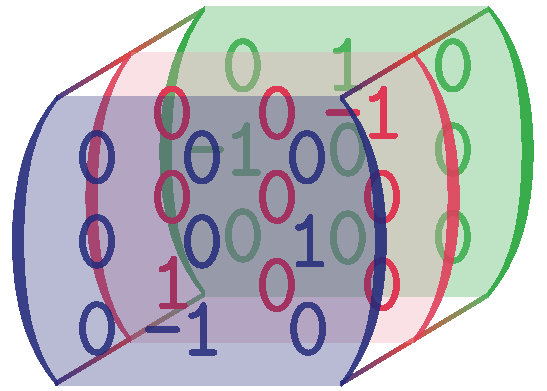
\includegraphics[width=0.2\textwidth]{figures/epsilontensor.pdf}}}
    \quad 
    \mathbf{e}_i \otimes \mathbf{e}_j \otimes \mathbf{e}_k
\end{equation}

We may extend this concept further to higher orders. A stiffness tensor for example maps a second-order strain tensor to a second-order stress tensor and thus it is a fourth-order tensor, which we denote with double-stroke capital letters. More general, a fourth order tensor may be obtained by an outer product of two second-order tensors $\mathbf{A},\mathbf{B}\in \mathcal{R}^{d \times d} \rightarrow \mathcal{R}^{d \times d \times d \times d}$ as 
\begin{equation}
    \mathbb{C} = \mathbf{A} \otimes \mathbf{B} = \sum_{i,j,k,l} A_{ij}B_{kl}  \mathbf{e}_i \otimes \mathbf{e}_j \otimes \mathbf{e}_k \otimes \mathbf{e}_l.
\end{equation}

We define the tensor contraction of two second-order tensors $\mathbf{A},\mathbf{B} \in \mathcal{R}^{d \times d} \rightarrow \mathcal{R}^{d \times d}$: 
\begin{align}
    \mathbf{A} \cdot \mathbf{B} 
        &= \sum_{i,j} A_{ij} \mathbf{e}_i \otimes \mathbf{e}_j \cdot \sum_{k,l}B_{kl} \mathbf{e}_k \otimes \mathbf{e}_l \\
        &= \sum_{i,j,k,l} A_{ij} B_{kl} (\mathbf{e}_i \otimes \overbracket{\mathbf{e}_j) \cdot  (\mathbf{e}_k}^{\delta_{jk}} \otimes \mathbf{e}_l) \\
        &= \sum_{i,j,k,l} A_{ij} B_{kl} (\overbracket{\mathbf{e}_j \cdot  \mathbf{e}_k}^{\delta_{jk}}) \mathbf{e}_i \otimes \mathbf{e}_l \\
        &= \sum_{i,j,k,l} A_{ij}B_{kl} \delta_{jk} \mathbf{e}_i \otimes \mathbf{e}_l \\
        &= \sum_{i,j,l} A_{ij}B_{jl} \mathbf{e}_i \otimes \mathbf{e}_l
\end{align}
Essentially, this contracts the inner dimensions. This is an exemplary summary of such contractions:

\begin{example}{Tensor contraction}{tensorcontractionexample}
    Contraction of two first order tensors $\mathbf{a},\mathbf{b} \in \mathcal{R}^d \rightarrow \mathcal{R}$: 
    \begin{equation}
        \mathbf{a} \cdot \mathbf{b} = \sum_i a_i b_i 
    \end{equation}
    Contraction of two second-order tensors $\mathbf{A},\mathbf{B} \in \mathcal{R}^{d \times d} \rightarrow \cdot \mathcal{R}^{d \times d}$: 
    \begin{equation}
        \mathbf{A} \cdot \mathbf{B} = \sum_{i,j,k} A_{ij} B_{jk} \mathbf{e}_i \otimes \mathbf{e}_k
    \end{equation}
    Contraction of a second-order tensor $\mathbf{A} \in \mathcal{R}^{d \times d}$ and a first-order tensor $\mathbf{b} \in \mathcal{R}^d \rightarrow \mathcal{R}^d$: 
    \begin{equation}
        \mathbf{A} \cdot \mathbf{b} = \sum_{i,j} A_{ij} b_j \mathbf{e}_i 
    \end{equation}
\end{example}

We can apply the inner product multiple times. For example, we can define the double contraction of two second-order tensors $\mathbf{A},\mathbf{B} \in \mathcal{R}^{d \times d} \rightarrow \mathcal{R}$: 
\begin{align}
    \mathbf{A} : \mathbf{B} 
        &= \sum_{i,j} A_{ij} \mathbf{e}_i \otimes \mathbf{e}_j :  \sum_{k,l} B_{kl} \mathbf{e}_k \otimes \mathbf{e}_l \\
        &= \sum_{i,j,k,l} A_{ij}B_{kl} (\underbracket{\mathbf{e}_i \otimes \overbracket{\mathbf{e}_j) :  (\mathbf{e}_k}^{\delta_{jk}} \otimes \mathbf{e}_l}_{\delta_{il}}) \\
        &= \sum_{i,j,k,l} A_{ij}B_{kl} \delta_{jk} \delta_{il} \\
        &= \sum_{i,j} A_{ij}B_{ji}
\end{align}

Essentially, the number of dots in the product indicates how many dimensions we want to contract.

\begin{example}{Tensor double contraction}{tensordoublecontractionexample}
    Double contraction of two second-order tensors $\mathbf{A},\mathbf{B} \in \mathcal{R}^{d \times d} \rightarrow \mathcal{R}$: 
    \begin{equation}
        \mathbf{A} : \mathbf{B} = \sum_{i,j} A_{ij} B_{ji} 
    \end{equation}
    Double contraction of two fourth-order tensors $\mathbb{A},\mathbb{B} \in \mathcal{R}^{d \times d \times d \times d} \rightarrow \mathcal{R}^{d \times d \times d \times d}$: 
    \begin{equation}
        \mathbb{A} : \mathbb{B} = \sum_{i,j,k,l,m,n} A_{ijkl} B_{lkmn} \mathbf{e}_i \otimes \mathbf{e}_j \otimes \mathbf{e}_m \otimes \mathbf{e}_n
    \end{equation}
    Double contraction of a fourth-order tensor $\mathbb{A} \in \mathcal{R}^{d \times d \times d \times d}$ and a second-order tensor $\mathbf{B} \in \mathcal{R}^{d \times d} \rightarrow \mathcal{R}^{d \times d}$: 
    \begin{equation}
        \mathbb{A} : \mathbf{B} = \sum_{i,j,k,l} A_{ijkl} B_{lk} \mathbf{e}_i \otimes \mathbf{e}_j
    \end{equation}
\end{example}

Finally, we denote the trace, transposition and inverse of a tensor as $\text{tr}(\mathbf{A})$, $\mathbf{A}^\top$, and $\mathbf{A}^{-1}$, respectively.

\section{Tensor analysis}
In many physical processes, variables appear as \emph{tensor fields} with a dependency on a spatial variable $\mathbf{x} \in \mathcal{R}^d$. Some examples are given here:
\begin{example}{Tensor fields}{tensorfieldexample}
    A temperature field is a scalar field
    \begin{equation}
        \theta: \mathcal{R}^d \rightarrow \mathcal{R}.
    \end{equation}
    A displacement field is a vector field
    \begin{equation}
        \mathbf{u}: \mathcal{R}^d \rightarrow \mathcal{R}^d.
    \end{equation}
    A stress field is a second-order tensor field
    \begin{equation}
        \mathbf{S}: \mathcal{R}^d \rightarrow \mathcal{R}^{d \times d}.
    \end{equation}
\end{example}

In most governing equations of physical processes, we need to compute differential operations on these fields. Therefore, the following sections introduce the most important differential operators for tensor fields assuming that the fields are differentiable and that we are using Cartesian coordinates \footnote{In curvilinear coordinates things get a bit more complicated. We stick to Cartesian coordinated in this lecture. }. 

A common notation for differential operations on tensor fields utilizes the Nabla operator 
\begin{equation}
    \nabla = \sum_i \frac{\partial }{\partial x_i} \mathbf{e}_i = 
    \begin{pmatrix}
            \frac{\partial}{\partial x_1} \\
            \frac{\partial}{\partial x_2} \\
            \dots \\
            \frac{\partial}{\partial x_d} \\
        \end{pmatrix}_{\{\mathbf{e}_i\}}
\end{equation}
The Nabla operator may be interpreted as a first-order tensor or vector, which upon multiplication in an inner product or cross product applies a derivative instead of being just multiplied. 

\subsection{Gradient}
The gradient computes the partial derivative with respect to each spatial direction and represents this information as a higher-order tensor. We denote the gradient operator $\nabla (\bullet)$. The resulting tensor is increased by one order as shown in the following examples:
\begin{example}{Gradient}{gradientsexample}
    Gradient of a scalar field
    \begin{equation}
        \nabla \theta = \sum_i \frac{\partial \theta}{\partial x_i} \mathbf{e}_i =
        \begin{pmatrix}
            \frac{\partial \theta}{\partial x_1} \\
            \frac{\partial \theta}{\partial x_2} \\
            \dots \\
            \frac{\partial \theta}{\partial x_d} \\
        \end{pmatrix}_{\{\mathbf{e}_i\}}
    \end{equation}
    Gradient of a vector field
    \begin{equation}
        \nabla \mathbf{u} = \sum_{i,j} \frac{\partial u_i}{\partial x_j} \mathbf{e}_i \otimes \mathbf{e}_j
        = 
        \begin{pmatrix}
            \frac{\partial u_1}{\partial x_1} & \frac{\partial u_1}{\partial x_2} & \dots & \frac{\partial u_1}{\partial x_d}\\
            \frac{\partial u_2}{\partial x_1} & \frac{\partial u_2}{\partial x_2} & \dots & \frac{\partial u_2}{\partial x_d}\\
            \dots & \dots & \dots & \dots\\
            \frac{\partial u_d}{\partial x_1} & \frac{\partial u_d}{\partial x_2} & \dots & \frac{\partial u_d}{\partial x_d}\\
        \end{pmatrix}_{\{\mathbf{e}_i\}}
    \end{equation}
\end{example}

The gradient may be interpreted as a measure for how much a tensor changes in each direction. 

We may compute the gradient of a gradient of a scalar field. If all the partial derivatives exits, we call the entries a \emph{Hessian}.

\begin{example}{Hessian}{hessianexample}
    Hessian of a scalar field
    \begin{equation}
        \nabla^2 \theta = \sum_{i,j} \frac{\partial^2 \theta}{\partial x_i \partial x_j} \mathbf{e}_i \otimes \mathbf{e}_j
        = 
        \begin{pmatrix}
            \frac{\partial^2 \theta}{\partial x_1 \partial x_1} & \frac{\partial^2 \theta}{\partial x_1 \partial x_2} & \dots & \frac{\partial^2 \theta}{\partial x_1 \partial x_d}\\
            \frac{\partial^2 \theta}{\partial x_2 \partial x_1} & \frac{\partial^2 \theta}{\partial x_2 \partial x_2} & \dots & \frac{\partial^2 \theta}{\partial x_2 \partial x_d}\\
            \dots & \dots & \dots & \dots\\
            \frac{\partial^2 \theta}{\partial x_d \partial x_1} & \frac{\partial^2 \theta}{\partial x_d \partial x_2} & \dots & \frac{\partial^2 \theta}{\partial x_d \partial x_d}\\
        \end{pmatrix}_{\{\mathbf{e}_i\}}
    \end{equation}
\end{example}

\subsection{Divergence}
The divergence computes the partial derivative with respect to each spatial direction, sums these values up and represents this information as a lower-order tensor. We denote the divergence operator $\nabla \cdot (\bullet)$. The resulting tensor is increased by one order as shown in the following examples:
\begin{example}{Divergence}{divergenceexample}
    Divergence of a vector field
    \begin{equation}
        \nabla \cdot \mathbf{u} =  \sum_i \frac{\partial u_i}{\partial x_i}
        = 
        \frac{\partial u_1}{\partial x_1} + \frac{\partial u_2}{\partial x_2} + \dots + \frac{\partial u_d}{\partial x_d}
    \end{equation}
    Divergence of a second-order tensor field
    \begin{equation}
        \nabla \cdot \mathbf{S} = \sum_{i,j} \frac{\partial S_{ij}}{\partial x_j} \mathbf{e}_i
        = 
        \begin{pmatrix}
            \frac{\partial S_{11}}{\partial x_1} + \frac{\partial S_{12}}{\partial x_2} + \frac{\partial S_{13}}{\partial x_3} \\
            \frac{\partial S_{21}}{\partial x_1} + \frac{\partial S_{22}}{\partial x_2} + \frac{\partial S_{23}}{\partial x_3}\\
            \frac{\partial S_{31}}{\partial x_1} + \frac{\partial S_{32}}{\partial x_2} + \frac{\partial S_{33}}{\partial x_3}
        \end{pmatrix}_{\{\mathbf{e}_i\}}
    \end{equation}
\end{example}

The divergence may be interpreted as the tensor field's source. If the divergence is positive, this is a source and if it is negative, it will act as a sink. 

\bibliographystyle{unsrtnat}
\bibliography{literature} 

% SEE https://biomechanics.stanford.edu/me337/me337_s02.pdf
\chapter{Unconstrained optimization}
Optimization is the search for a minimum or maximum of some objective function. In fact, we can focus on minimization only, because maximization can be transferred to minimization by multiplying the objective function with $-1$. 
We are familiar with such problems from basic math courses in which we learned that the minimum of a continuous differentiable function $f(x)$ fulfills the necessary condition $f'(x)=0$ and the sufficient condition $f''(x) > 0$. 

Here, we extend this concept to a multi-dimensional optimization variable $\mathbf{x} \in \mathcal{R}^d$ and formulate the optimization problem as 
\begin{equation}
    \min_{\mathbf{x}} \quad f(\mathbf{x})
   \label{eq:unconstrained_optimzation}
\end{equation}
with $f: \mathcal{R}^d \rightarrow \mathcal{R}$.

We may use an analogy at this point: \emph{Consider a person hiking in the mountains and the height of the mountains is described by a function $f$ that depends on the location $\mathbf{x}$. The person can go anywhere in the mountain range $\mathcal{R}^d$ without restrictions, but wants to get back to the village, which is located at the bottom of the deepest valley at position $\mathbf{x}^*$. To get to the location of that village, the person needs to solve Equation \eqref{eq:unconstrained_optimzation}.}

\begin{objectives}{}{objectives_unconstrained_optimization}
After studying this chapter and finishing the exercise, you should be able to 
\begin{itemize}[label=$\dots$]
    \item distinguish the local and global optimum
    \item define convexity of sets and functions
    \item explain gradient decent methods such as simple steepest decent, steepest decent with incomplete line search, conjugated gradients, and quasi Newton 
    \item implement these gradient decent methods in computer code
\end{itemize}
\end{objectives}

\section{Local and global optimum}
As mentioned earlier, we may interpret the problem \eqref{eq:unconstrained_optimzation} as searching for the lowest point $\mathbf{x}^* \in \mathcal{R}^d$ in a mountainous landscape, as illustrated in Figure \ref{fig:global_local_optimization}. 

This lowest point is termed \emph{global minimum}, if 
\begin{equation}
    f(\mathbf{x}^*) \le f(\mathbf{x})  \quad \forall \mathbf{x} \in \mathcal{R}^d.
\end{equation}
However, finding this global minimum is generally a challenging task, because it is computationally demanding to test all points against all other points. 

\begin{figure}
    \centering
    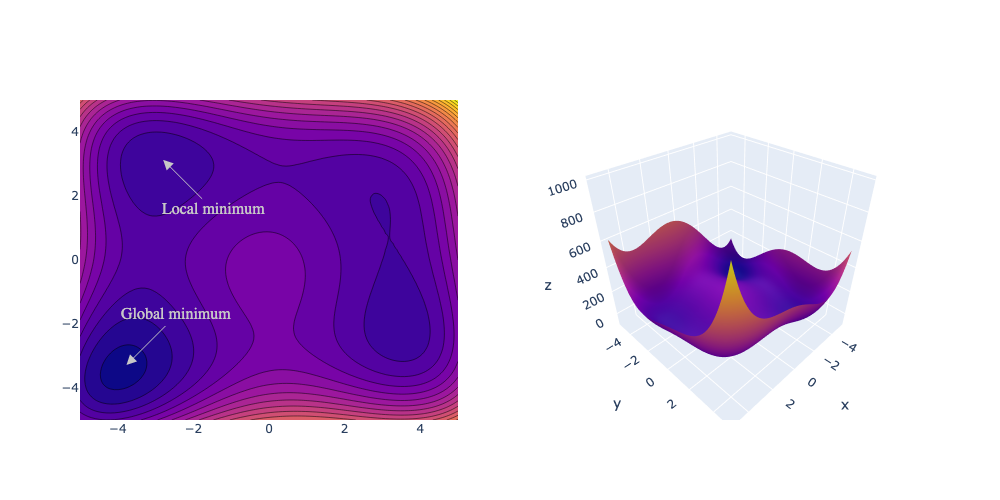
\includegraphics[width=\textwidth]{figures/opti_landscape.png}
    \caption{Global and local optimum in an optimization problem.}
    \label{fig:global_local_optimization}
\end{figure}

Hence, we focus on the easier problem of trying to find \emph{local minima}, i.e. points which are lower or equal in a local neighborhood. A local minimum is located at a stationary point 
\begin{equation}
    \nabla f(\mathbf{x}^*) = \mathbf{0},
    \label{eq:stationary_point}
\end{equation}
even though not all stationary points are local minima (they could be a maximum or saddle points).
Of course, the global minimum is also a local minimum, but under which conditions is the local minimum also a global minimum? The answer to this question is "in \emph{convex problems}" and is explored in the next section.

\section{Convexity}
A set $\mathcal{S} \subset \mathcal{R}^d$ is termed \emph{convex}, if 
\begin{equation}
    \lambda \hat{\mathbf{x}} + (1-\lambda) \check{\mathbf{x}} \in \mathcal{S} \quad \forall \hat{\mathbf{x}}, \check{\mathbf{x}} \in \mathcal{S} \quad  \forall \lambda \in [0,1].
\end{equation}
This means, we are able to draw a straight line from any point in the set to another point in the set, in which any point at the line is still in the set (see Figure \ref{fig:convex_sets}).

\begin{figure}[!htpb]
    \centering
    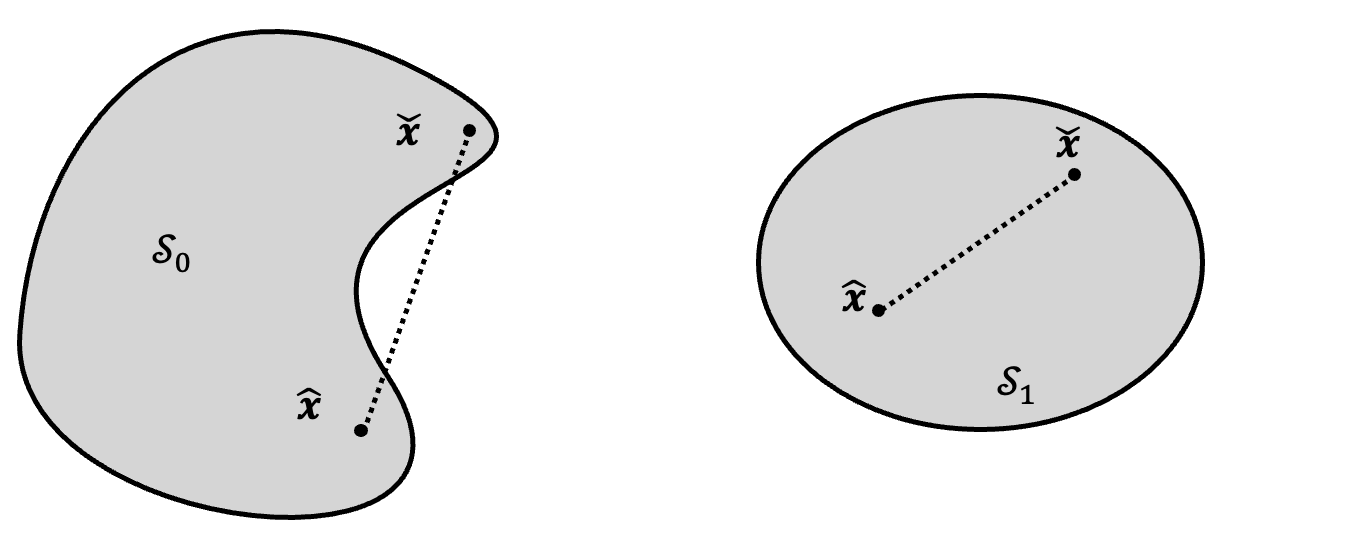
\includegraphics[width=0.8\textwidth]{figures/convex_sets.png}
    \caption{Set $\mathcal{S}_0$ is not convex, set $\mathcal{S}_1$ is convex.}
    \label{fig:convex_sets}
\end{figure}

A function $f: \mathcal{S} \rightarrow \mathcal{R}$ is termed strictly convex on a convex set $\mathcal{S}$, if 
\begin{equation}
    f(\lambda \hat{\mathbf{x}} + (1-\lambda) \check{\mathbf{x}}) <  \lambda f(\hat{\mathbf{x}}) + (1-\lambda) f(\check{\mathbf{x}}) \quad \forall \hat{\mathbf{x}}, \check{\mathbf{x}} \in \mathcal{S} \quad  \forall \lambda \in [0,1].
\end{equation}
We can asses the convexity of a function $f: \mathcal{S} \rightarrow \mathcal{R}$ on a convex set $\mathcal{S}$ by checking its Hessian $\nabla^2 f$. If the Hessian matrix is positive definite ($\mathbf{y} \cdot \nabla^2 f \cdot  \mathbf{y} > 0 \forall \mathbf{y}$) for all points in $\mathcal{S}$,  $f$ is strictly convex.

\begin{example}{Convex functions}{convexfunctionexample}
    The function $f(\mathbf{x})=x_1^2 + x_2^2$ is convex, as its Hessian \begin{equation}
        \nabla^2f(\mathbf{x}) = 
        \begin{pmatrix}
        2 & 0 \\ 
        0       & 2         
        \end{pmatrix}
    \end{equation} 
    is positive definite. Visually this means, we can draw a line between any two points of the function and it will never intersect the function.

    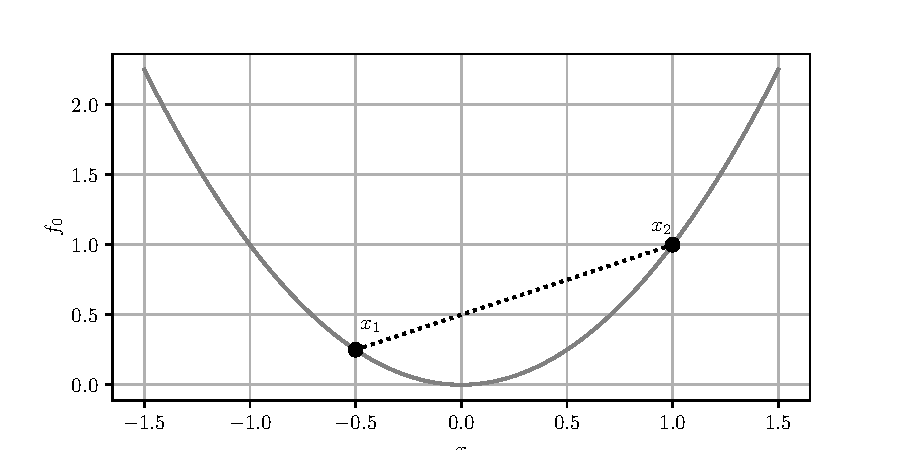
\includegraphics[width=\textwidth]{figures/convex_function_0.pdf}
\end{example}


\begin{example}{Non-convex functions}{nonconvexfunctionexample}
    The function $f(x, y)=x_1^4-x_1^2+x_2^2$ is not strictly convex, because its Hessian 
    \begin{equation}
        \nabla^2f(\mathbf{x}) = 
        \begin{pmatrix}
        12x_1^2-2 & 0 \\ 
        0       & 2         
        \end{pmatrix}
    \end{equation} 
    is not positive definite. Visually this means, we can find two points, for which drawing a line between them would cross the function. 
    
    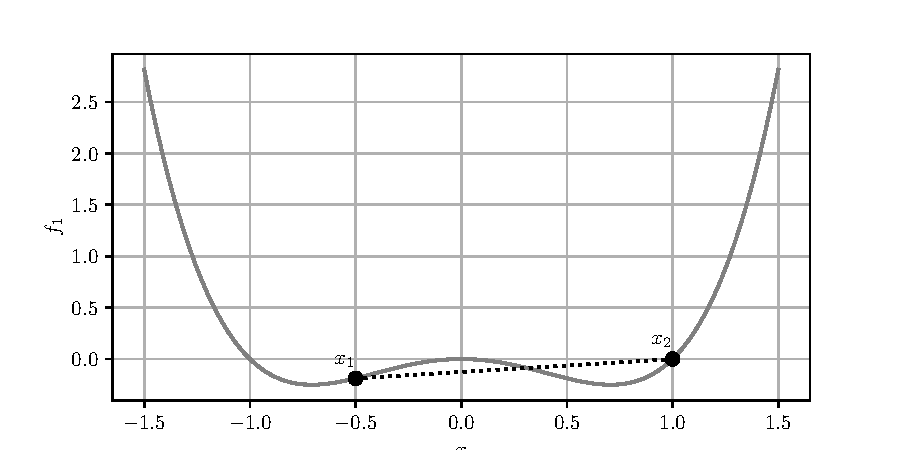
\includegraphics[width=\textwidth]{figures/convex_function_1.pdf}
\end{example}

An unconstrained optimization problem is termed \emph{convex}, if the objective function $f: \mathcal{S} \rightarrow \mathcal{R}$ is convex and the set $\mathcal{S}$ is convex. If in addition, the set $\mathcal{S}$ is compact (i.e. bounded and closed), there exists exactly one solution for the optimization problem. In conclusion this means, that finding the local minimum in a convex problem is equivalent to finding its global minimum. 

\section{Gradient decent methods}
For analytical convex problems, we only have to find a stationary point (see Equation \ref{eq:stationary_point}) by finding the gradient of the objective function and finding the point where it is vanishing. This requires an explicit differentiable expression of the objective function, which is then rearranged.

However, such an explicit expression of the objective function is not always readily available - e.g. if the objective function is an artificial neural network or a numerical simulation model. In these cases, we are usually just able to compute a local gradient in the vicinity of a point, but are not able to find a closed expression for the gradient. 

An analogy to that would be the search for a minimum in a mountainous landscape with heavy fog: \emph{A person hiking in foggy mountains would be able to only evaluate the height and steepness of the mountains in its close neighborhood. The evaluation of height and steepness takes some time, so the person also wants to find a strategy with a small number of measurements.}

\subsection{Simple steepest decent method}
An obvious approach to minimize such a "foggy" objective function is to follow the steepest gradient direction in order to find a better solution. In the image of searching the lowest point ins a hilly landscape, this is equivalent to descending a mountain by always walking in the direction directly perpendicular to the contour lines. 
A naive algorithm for this can be formulated as follows:
\begin{enumerate}
    \item Pick a starting point $\mathbf{x}^0$.
    \item Calculate the gradient $\nabla f(\mathbf{x}^k)$.
    \item Make a step $\mathbf{x}^{k+1} = \mathbf{x}^k -\eta \nabla f(\mathbf{x}^k)$.
    \item Repeat steps 2 and 3 until you reached a maximum number of iterations $k \le N$ or there is no improvement any more ($ \nabla f(\mathbf{x}^k) < \epsilon$). 
\end{enumerate}
The step itself is scaled with a factor $-\eta \in \mathcal{R}$. The sign stems from the fact that we want to minimize the function. The scaling variable $\eta$ is termed \emph{learning rate} in machine learning contexts and describes how large the step is before reevaluating the gradient again. A smaller learning rate improves convergence of the algorithm towards the exact solution, but requires more steps and more function evaluations. A larger value of $\eta$ makes it harder for the algorithm to converge, as it may "jump" over the minimum or may diverge. 

\begin{example}{Simple steepest decent}{simpledecentexample}
    We want to find the solution of the following quadratic unconstrained optimization problem
    \begin{equation}
        \begin{aligned}
            \min_{\mathbf{x}} \quad & f(\mathbf{x})= (\mathbf{x}-\tilde{\mathbf{x}}) \cdot \mathbf{Q} \cdot (\mathbf{x}-\tilde{\mathbf{x}})
        \end{aligned}
        \label{eq:simpledecent_example}
    \end{equation}
    with 
    \begin{equation}
        \mathbf{Q} = 
        \begin{pmatrix}
        2 & 1 \\
        1 & 1 
        \end{pmatrix}
        \quad \text{and} \quad
        \tilde{\mathbf{x}} = 
        \begin{pmatrix}
        -1\\
        1 
        \end{pmatrix}
        .
    \end{equation}

    The optimization path of a simple steepest decent method with a starting point $\mathbf{x}^0= (4, -1)^\top$ and $\eta=0.1$ is shown in the plot below with a blue line. However, the solution requires quite a lot of iterations.

    \begin{center}
        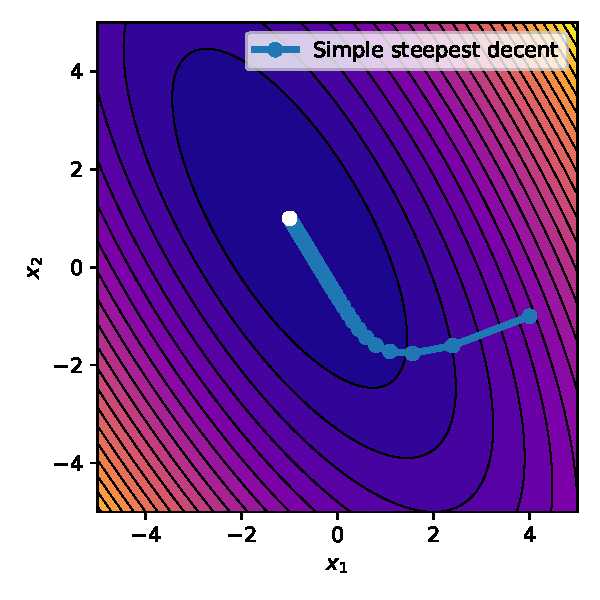
\includegraphics[width=0.5\textwidth]{figures/simple_decent.pdf}
    \end{center}   
\end{example}

\subsection{Steepest decent method with incomplete line search}
The previous approach is simple, but requires many repeated evaluations of the multi-dimensional gradient. Instead of going an arbitrary downhill step, it is more efficient to perform a line-search along the search direction to got this step towards the minimum in that direction: 
\begin{enumerate}
    \item Pick a starting point $\mathbf{x}^0$.
    \item Calculate the gradient $\nabla f(\mathbf{x}^k)$ and the search direction $\mathbf{p}^k = - \frac{\nabla f(\mathbf{x}^k)}{\lVert \nabla f(\mathbf{x}^k) \rVert}$.
    \item Solve the sub-problem $\min_{\eta} f(\mathbf{x}^k + \eta \mathbf{p}^k)$ to find the optimal step size $\eta$ for a fixed search direction $\mathbf{p}^k$.
    \item Make a step $\mathbf{x}^{k+1} = \mathbf{x}^k + \eta \mathbf{p}^k$.
    \item Repeat steps 2, 3 and 4 until you reached a maximum number of iterations $k \le N$ or there is no improvement any more ($ \nabla f(\mathbf{x}^k) < \epsilon$). 
\end{enumerate}

The sub-problem is just a one-dimensional optimization problem. However, it still requires an iterative solution, if the resulting function $f(\mathbf{x}^k + \eta \mathbf{p}^k)$ has no analytical expression w.r.t. $\eta$. Hence solving this problem to its exact value still takes some time. We do not need to solve this sub-problem to its exact optimal value, though. We can search for a solution that is "good enough" and save some time. But what is good enough?
There are a couple of criteria to stop an optimization early, one of which is the \emph{Armijo condition} 
\begin{equation}
    f(\mathbf{x}^k + \eta \mathbf{p}^k) \le f(\mathbf{x}^k) + c \eta  \nabla f(\mathbf{x}^k) \cdot \mathbf{p}^k 
\end{equation}
with $c \in (0,1)$. This condition ensures a sufficient decrease of the objective function value assuming that we can expect more decrease if the gradient is larger. 

\begin{example}{Armijo condition}{armijoexample}
    Consider the function $f(x)$ displayed below. The Armijo condition is satisfied in all green ranges.  
    
    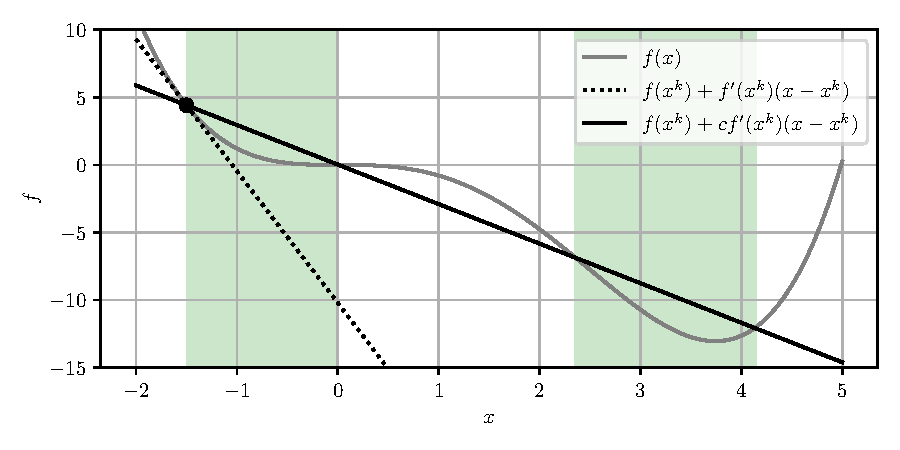
\includegraphics[width=\textwidth]{figures/armijo_condition.pdf}
\end{example}

The Armijo condition is always fulfilled for very small steps, thus we have to consider an additional curvature condition (in combination, these are called \emph{Wolfe conditions}) or implement the condition in a clever way to allow for a sufficiently large step size. Latter can be realized with the \emph{backtracking method}, which is usually used to perform the line search to find the step width: 
\begin{enumerate}
    \item Choose $\eta^0$, e.g. $\eta^0=1$.
    \item Evaluate the Armijo condition $f(\mathbf{x}^k + \eta^k \mathbf{p}^k) \le f(\mathbf{x}^k) + c \eta^k \nabla f(\mathbf{x}^k) \cdot \mathbf{p}^k $
    \item If the condition is fulfilled, we have found a suitable $\eta$, else we try step 2 with a new parameter $\eta^{k+1}=\rho \eta^k$ with a contraction factor $\rho \in (0,1)$ again.
\end{enumerate}
This algorithm usually provides a good compromise, as it provides a sufficiently small step to achieve a valid sufficient decrease, but is still large enough to make reasonable progress towards convergence.

The proposed steepest decent method is a useful strategy for unconstrained optimization problems. However, it can be slow because subsequent search directions are perpendicular to each other and search may take many iterations.

\begin{example}{Steepest decent with incomplete line search}{steepestdecentexample}
    We consider the optimization of Equation \eqref{eq:simpledecent_example} using a steepest decent method with incomplete line search. The optimization path for a starting point $\mathbf{x}^0= (4, -1)^\top$, $\eta^0=5.0$, $c=0.5$, and $\rho=0.8$ is shown in the plot below with a blue line. The solution converges much faster than the simple steepest decent.
    \begin{center}
        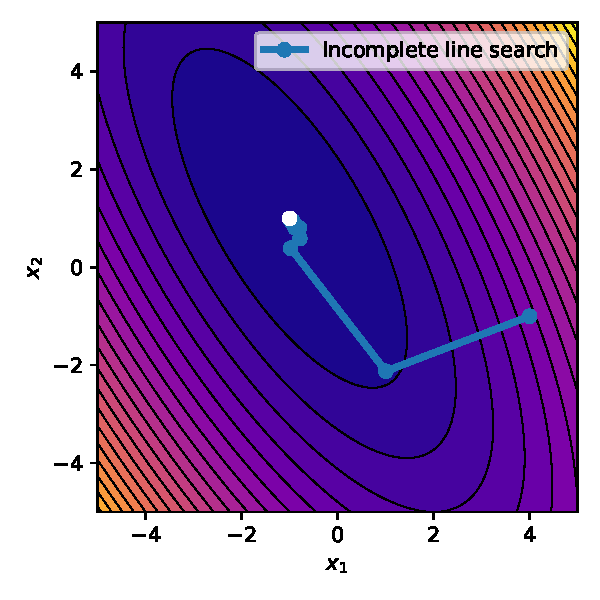
\includegraphics[width=0.5\textwidth]{figures/steepest_decent.pdf}
    \end{center}   
\end{example}

\subsection{Conjugated gradients method}
Especially near the optimum, the steepest decent may lead to a "zig-zag" pattern and many iterations. We can improve the algorithm by ensuring that search directions are conjugated directions to the Hessian of that function. For quadratic problems of the form $f(\mathbf{x}) = \mathbf{x} \cdot \mathbf{A} \cdot \mathbf{x} - \mathbf{b} \mathbf{x}$, this ensures that we can reach the optimum for $\mathbf{x} \in \mathcal{R}^d$ in $d$ steps.

The algorithm of a conjugated gradient method according to Fletchers and Reeves \cite{Fletcher1964} is as follows: 
\begin{enumerate}
    \item Pick a starting point $\mathbf{x}^0$.
    \item Calculate the gradient $\nabla f(\mathbf{x}^k)$.
    \item Compute a conjugate direction $\mathbf{p}^k = -\nabla f(\mathbf{x}^k) + \beta \mathbf{p}^{k-1}$ with  
    \begin{equation}
        \beta = \frac{\nabla f(\mathbf{x}^k) \cdot \nabla f(\mathbf{x}^k)}{\nabla f(\mathbf{x}^{k-1}) \cdot \nabla f(\mathbf{x}^{k-1})}.
    \end{equation}
    \item Solve the sub-problem $\min_{\eta} f(\mathbf{x}^k + \eta \mathbf{p}^k)$ to find the optimal step size $\eta$ for a fixed search direction $\mathbf{p}^k$.
    \item Make a step $\mathbf{x}^{k+1} = \mathbf{x}^k + \eta \mathbf{p}^k$.
    \item Repeat steps 2, 3, 4 and 5 until you reached a maximum number of iterations $k \le N$ or there is no improvement any more ($ \nabla f(\mathbf{x}^k) < \epsilon$). 
\end{enumerate}

\begin{example}{Conjugated gradients}{cgexample}
    We consider the optimization of Equation \eqref{eq:simpledecent_example} using the CG method with incomplete line search for the sub-problem. The optimization path for a starting point $\mathbf{x}^0= (4, -1)^\top$, $\eta^0=5.0$, $c=0.5$, and $\rho=0.8$ is shown in the plot below with a blue line. The solution converges in just two iterations for this 2D problem, as the problem is quadratic.
    \begin{center}
        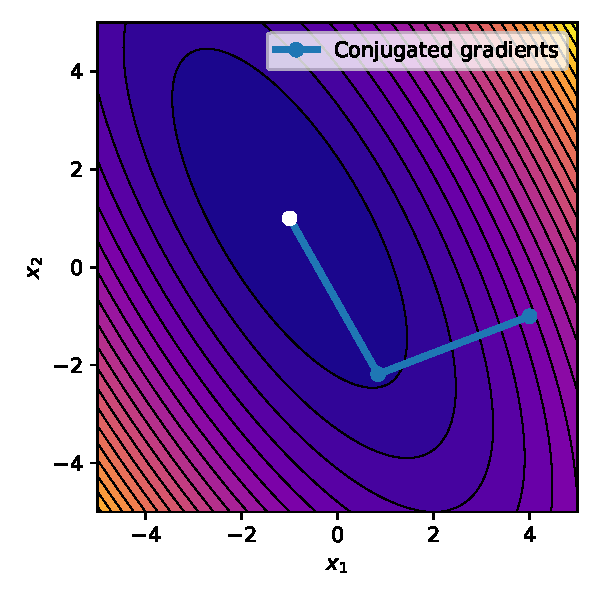
\includegraphics[width=0.5\textwidth]{figures/cg.pdf}
    \end{center}   
\end{example}

\subsection{Quasi Newton methods}
Newton's method is a well known method to find roots of a function. 

\begin{example}{Newton's method}{newtonexample}
    Consider the nonlinear function $f(x) = x^2 - 3$ displayed below. To find a root, i.e. the values of $x$ where $f(x)=0$, we can employ Newtons method: 
    \begin{enumerate}
        \item Pick a starting point $x^0$.
        \item Compute the derivative $f'(x)$.
        \item Compute a new point $x^{k+1} = x^k - \frac{f(x^k)}{f'(x^k)}$.
        \item Repeat the steps 2 and 3 until converged.
    \end{enumerate}
    
    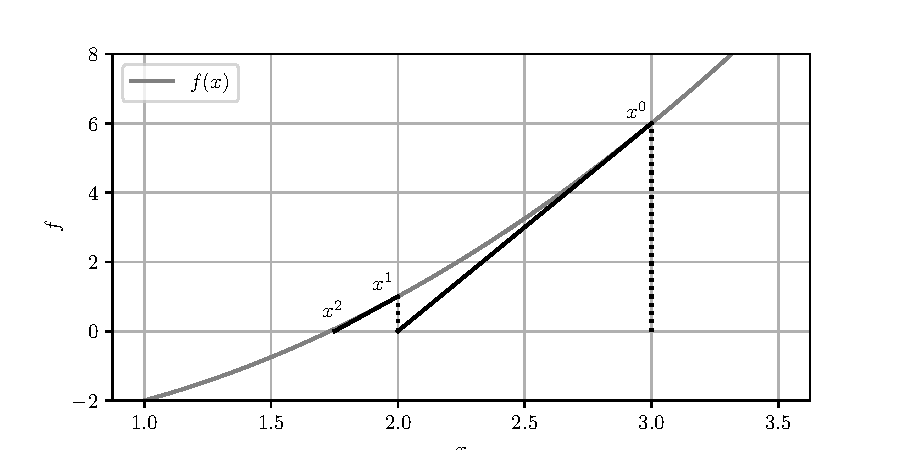
\includegraphics[width=\textwidth]{figures/netwon_iteration.pdf}
    \begin{center}    
        \begin{tabular}{cccc}
    
             Iteration  & $x^k$     & $f(x^k)$  & $f'(x^k)$\\
             \hline
             0          & 3.0       & 6.0       & 6.0\\
             1          & 2.0       & 1.0       & 4.0\\
             2          & 1.75      & 0.0625    & 3.5\\
             3          & 1.7314    & \dots     & \dots\\
        \end{tabular}
    \end{center}
\end{example}


We can utilize Newton's method to find roots of the first derivative of a function, which are stationary points and thus in case of convexity global minima.
We therefore solve the problem 
\begin{equation}
    \nabla f(\mathbf{x}) = \nabla f(\mathbf{x}^k) + \underbrace{\nabla^2 f(\mathbf{x}^k)}_{\mathbf{H}} (\mathbf{x}-\mathbf{x}^k) = 0
\end{equation}
with Newton's iteration procedure 
\begin{equation}
    \mathbf{x}^{k+1} = \mathbf{x}^k  - \mathbf{H}^{-1} \nabla f(\mathbf{x}^k) 
\end{equation}
starting from a starting point $\mathbf{x}^0$. For a quadratic problem, this method would find the solution immediately. However, the inverse Hessian $\mathbf{H}^{-1}$ is computationally expensive to obtain. We use an alternative to computing this term, hence the following method is a "quasi" Newton method. 

We can build up $\mathbf{H}^{-1}$ iteratively in the Broyden–Fletcher–Goldfarb–Shanno (BFGS) \cite{Broyden1970, Fletcher1970, Goldfarb1970, Shanno1970} algorithm: 
\begin{enumerate}
    \item Pick a starting point $\mathbf{x}^0$ and set $(\mathbf{H}^{-1})^0=\mathbf{I}$.
    \item Calculate the gradient $\nabla f(\mathbf{x}^k)$ and compute the direction $\mathbf{p}^k = - (\mathbf{H}^{-1})^0 \nabla f(\mathbf{x}^k)$.
    \item Solve the sub-problem $\min_{\eta} f(\mathbf{x}^k + \eta \mathbf{p}^k)$ to find the optimal step size $\eta$ for a fixed search direction $\mathbf{p}^k$.
    \item Make a step $\mathbf{x}^{k+1} = \mathbf{x}^k + \eta \mathbf{p}^k$.
    \item Compute the difference of gradients $ \mathbf{y}^k = \nabla f(\mathbf{x}^{k+1}) - \nabla f(\mathbf{x}^k)$.
    \item Update the inverse Hessian 
    \begin{equation}
        \nonumber
        (\mathbf{H}^{-1})^{k+1} = 
            \left(\mathbf{I} - \frac{\mathbf{p}^k \otimes \mathbf{y}^k}{\mathbf{p}^k \cdot \mathbf{y}^k} \right)
            \cdot
            (\mathbf{H}^{-1})^k
            \cdot
            \left(\mathbf{I} - \frac{\mathbf{y}^k \otimes \mathbf{p}^k}{\mathbf{p}^k \cdot \mathbf{y}^k} \right) 
            + 
            \frac{\mathbf{p}^k \otimes \mathbf{p}^k}{\mathbf{p}^k \cdot \mathbf{y}^k}
    \end{equation}
    \item Repeat steps 2, 3 and 4 until you reached a maximum number of iterations $k \le N$ or there is no improvement any more ($ \nabla f(\mathbf{x}^k) < \epsilon$). 
\end{enumerate}

\begin{example}{BFGS}{bfgsexample}
    We consider the optimization of Equation \eqref{eq:simpledecent_example} using the BFGS method with incomplete line search for the sub-problem. The optimization path for a starting point $\mathbf{x}^0= (4, -1)^\top$, $\eta^0=5.0$, $c=0.5$, and $\rho=0.8$ is shown in the plot below with a blue line. The solution converges in just two iterations for this 2D quadratic problem.
    \begin{center}
        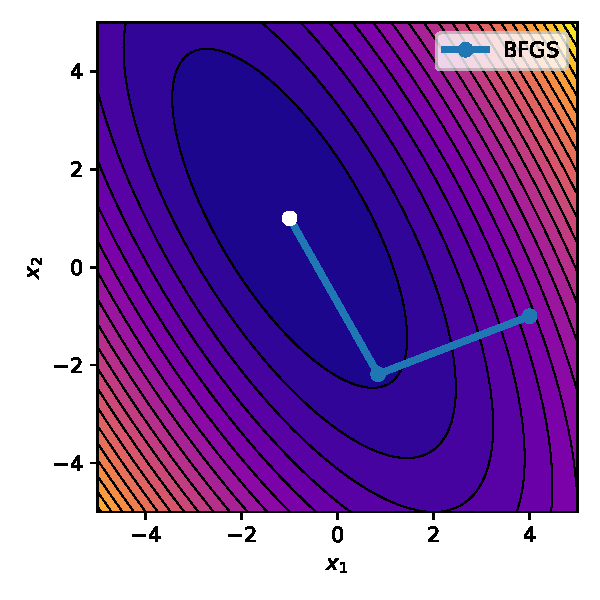
\includegraphics[width=0.5\textwidth]{figures/bfgs.pdf}
    \end{center}   
\end{example}


\bibliographystyle{unsrtnat}
\bibliography{literature} 


% https://optimization.cbe.cornell.edu/index.php?title=Main_Page
\chapter{Constrained optimization}
In the previous chapter, we draw the analogy between an optimization problem and the search for the lowest point in a mountainous landscape. We may continue with this analogy and make it a bit more realistic: \emph{Previously, the hiking person was able to access any point in the mountain range $\mathcal{S}$. However, in reality we might find a couple of constrains in that mountainous landscape. Someone might have put fences in the landscape and we are not able to cross these fences or we are restricted to a hiking path and cannot leave that path.}

These additional constraints make the optimization harder - the optimum that is achievable for us might be just "at a fence" and not the global optimum of the unrestricted function.
We denote the general form of a constrained optimization problem as 
\begin{equation}
    \begin{aligned}
        \min_{\mathbf{x}} \quad & f(\mathbf{x})\\
        \textrm{s.t.} \quad & g_i(\mathbf{x}) \le 0    &i \in [1, n]\\
                            & h_j(\mathbf{x}) = 0  &j \in [1, m]\\
                            & \mathbf{x} \in \mathcal{X} \subset \mathcal{R}^d\\
    \end{aligned}
    \label{eq:constrained_optimization}
\end{equation}
with $n$ inequality constraints $g_i : \mathcal{X} \rightarrow \mathcal{R}$ ("fences"), $m$ equality constraints $h_j: \mathcal{X} \rightarrow \mathcal{R}$ ("hiking paths") and a box constraint $\mathbf{x} \in \mathcal{X}$ ("allowed zone" in the mountain range). A constrained optimization problem is strictly convex, if the set $\mathcal{X}$ is strictly convex, the objective function is strictly convex and the constraints are strictly convex.

\begin{objectives}{}{objectives_constrained_optimization}
After studying this chapter and finishing the exercise, you should be able to 
\begin{itemize}[label=$\dots$]
    \item treat box constraints in gradient decent methods with projected gradients
    \item formulate Lagrangian functions of constrained optimization problems
    \item apply the Karush-Kuhn Tucker conditions to find the optimum of a convex constrained optimization problem
    \item explain the term \emph{Lagangian duality} and in which cases the dual formulation is beneficial
    \item apply the Langragian duality method to solve convex separable problems
\end{itemize}
\end{objectives}

\section{Box constraints} 
First, we neglect the equality constraints and inequality constraints in the problem \eqref{eq:constrained_optimization}, i.e. $m=0, n=0$, and focus on box constraints $\mathbf{x} \in \mathcal{X}$. \emph{Box constraint} means that the variables are limited to an upper and lower bound $\mathbf{x}^u$ and $\mathbf{x}^l$, respectively. For example, design variables in structural optimization could be diameters of beams, which cannot become negative or should not exceed a certain maximum producible size.

These constraints are probably the most friendly constraints in an optimization problem and in a one-dimensional optimization problem we can deal with them simply by clipping the variable as 
\begin{equation}
    x^* = \max(\min(\hat{x}, x^u), x^l)
\end{equation}
with the stationary point $\hat{x}$, the lower bound $x_l$ and the upper bound $x_u$. However, clipping the stationary point in each dimension of a multi-dimensional problem would not result in the optimal point, as illustrated by the green point in the next example \cite{Niculae2020}.

One method to deal with box constrains in multi-dimensional optimization problems is the projected gradient method. In this method we project each step of a gradient decent back to the domain as 
\begin{equation}
    \mathbf{x}^{k+1} = P(\mathbf{x}^k -\eta \nabla f(\mathbf{x}^k))
\end{equation}
with a projection function $P: \mathcal{R}^d \rightarrow \mathcal{X}$. In case of box constraints, this projection is simply clipping the values to $\mathcal{X}$ by 
\begin{equation}
    P(\mathbf{x}) = \max(\min(\mathbf{x}, \mathbf{x}^u), \mathbf{x}^l),
\end{equation}
where the $\max()$ and $\min()$ operators perform a point-wise comparison. 

\begin{example}{Box constraints}{boxexample}
    We want to find the solution of the following quadratic optimization problem
    \begin{equation}
        \begin{aligned}
            \min_{\mathbf{x}} \quad & f(\mathbf{x})= (\mathbf{x}-\tilde{\mathbf{x}}) \cdot \mathbf{Q} \cdot (\mathbf{x}-\tilde{\mathbf{x}})\\
            \textrm{s.t.} \quad     & \mathbf{x}^l \le \mathbf{x} \le \mathbf{x}^u\\
        \end{aligned}
        \label{eq:boxexample}
    \end{equation}
    with 
    \begin{equation}
        \mathbf{Q} = 
        \begin{pmatrix}
        2 & 1 \\
        1 & 1 
        \end{pmatrix}
        ,
        \tilde{\mathbf{x}} = 
        \begin{pmatrix}
        -1\\
        1 
        \end{pmatrix}
        ,
        \mathbf{x}^l = 
        \begin{pmatrix}
        0\\
        -2 
        \end{pmatrix}
        ,
        \mathbf{x}^u = 
        \begin{pmatrix}
        2\\
        2 
        \end{pmatrix}
        .
    \end{equation}

    \begin{center}
        \includesvg[width=0.5\textwidth]{figures/box_example.svg}
    \end{center}

    This is visually equivalent to searching for that point $\mathbf{x}^*$ within the non-faded region in the displayed plot that has the smallest function value. In the unconstrained optimization problem, a simple steepest gradient decent follows the blue path and results in the blue point $(-1, 1)^\top$. In the constrained optimization problem, a simple steepest gradient decent follows the orange path and results in the orange point indicating the correct solution $(0, 0)^\top$ to problem \eqref{eq:boxexample}. Note that simply clipping the result $(-1, 1)^\top$ in each dimension would yield the position indicated by the green point, which is not the optimum.    
\end{example}


\section{Lagrange multipliers}
Now, we neglect only the inequality constraints in the problem \eqref{eq:constrained_optimization}, i.e. $n=0$. Then we can solve the problem using Lagrange multipliers. To do so, we formulate the Lagrangian function
\begin{equation}
    \mathcal{\mathcal{L}} (\mathbf{x}, \pmb{\lambda}) = f(\mathbf{x}) + \sum_{j=1}^m \lambda_j h_j(\mathbf{x}) 
\end{equation}
with so called Lagrangian multipliers $\pmb{\lambda} \in \mathcal{R}^m$. 
According to the Lagrange multiplier theorem, a stationary point of the Langrangian function 
\begin{align}
    \frac{\partial \mathcal{\mathcal{L}}}{\partial x_k} (\mathbf{x}^*, \pmb{\lambda}^*) &= \frac{\partial f }{\partial x_k} (\mathbf{x}^*) + \sum_{j=1}^m \lambda_j^* \frac{\partial h_j}{\partial x_k} (\mathbf{x}^*) = 0\\
    \frac{\partial \mathcal{\mathcal{L}}}{\partial \lambda_j} (\mathbf{x}^*, \pmb{\lambda}^*) &= h_j(\mathbf{x}^*) = 0,
\end{align}
fulfills the necessary condition to be an optimum of a constrained optimization problem, if the gradients of the equality constraints are linearly independent (\emph{Slater condition} or \emph{constraint qualification}). We may interpret these optimality conditions such that any directional derivative in a feasible direction becomes zero.

\begin{example}{Lagrange multipliers}{lagrangeexample}
    We want to find the solution of the following quadratic optimization problem for $\mathbf{x} \in \mathcal{R}^2$
    \begin{equation}
        \begin{aligned}
            \min_{\mathbf{x}} \quad & f(\mathbf{x})= (\mathbf{x}-\tilde{\mathbf{x}}) \cdot \mathbf{Q} \cdot (\mathbf{x}-\tilde{\mathbf{x}})\\
            \textrm{s.t.} \quad     & h(\mathbf{x}) = x_1 - x_2 - 2 = 0  \\
        \end{aligned}
    \end{equation}
    with 
    \begin{equation}
        \mathbf{Q} = 
        \begin{pmatrix}
        2 & 0 \\
        0 & 1 
        \end{pmatrix} 
        \quad 
        \text{and}
        \quad
        \tilde{\mathbf{x}} = 
        \begin{pmatrix}
        -1\\
        1 
        \end{pmatrix}.
    \end{equation}

    This is visually equivalent to searching for the point on the black line in the following image that has the smallest function value.
    \begin{center}
        \includesvg[width=0.5\textwidth]{figures/lagrange_example.svg}
    \end{center}

    We can find the solution to this problem by finding a stationary point of the Lagrangian function
    \begin{equation}
        \mathcal{\mathcal{L}}(\mathbf{x}, \lambda) = 2 (x_1-\tilde{x}_1)^2 + (x_2-\tilde{x}_2)^2 + \lambda (x_1 - x_2 -2)
    \end{equation}
    with its partial derivatives 
    \begin{align}
        \frac{\partial \mathcal{\mathcal{L}}}{\partial x_1} &= 4 x_1^* + \lambda^*  + 4 = 0\\
        \frac{\partial \mathcal{\mathcal{L}}}{\partial x_2} &= 2 x_2^* - \lambda^*  -2 = 0\\
        \frac{\partial \mathcal{\mathcal{L}}}{\partial \lambda} &= x_1^* - x_2^* -2 = 0.
    \end{align}
    This is a linear system of three equations with three unknowns and we can easily find the solution $x_1^*=\frac{1}{3} , x_1^*=-\frac{5}{3}, \lambda^*=-\frac{16}{3}$
\end{example}


\section{Karush-Kuhn-Tucker conditions}
The Lagrange multipliers where initially only defined for equality constraints. However, the concept can be extended to inequality constraints with a Lagrangian function 
\begin{equation}
    \mathcal{\mathcal{L}} (\mathbf{x}, \pmb{\mu}, \pmb{\lambda}) = f(\mathbf{x}) + \sum_{i=1}^n \mu_i g_i(\mathbf{x}) + \sum_{j=1}^m \lambda_j h_j(\mathbf{x}) 
\end{equation}
utilizing the Lagrangian multipliers $\pmb{\mu} \in \mathcal{R}^n$ and $\pmb{\lambda} \in \mathcal{R}^m$ \cite{Karush1939, Kuhn1951}.

Assuming that the gradients of the constraints are linearly independent, we can then formulate the Karush-Kuhn-Tucker (KKT) conditions as necessary conditions for an optimum of the optimization problem \eqref{eq:unconstrained_optimzation}: 
\begin{align}
    \frac{\partial \mathcal{\mathcal{L}}}{\partial x_k} (\mathbf{x}^*, \pmb{\mu}^*, \pmb{\lambda}^*) &= 
    \frac{\partial f }{\partial x_k} (\mathbf{x}^*) + \sum_{j=1}^n \mu_i^* \frac{\partial g_i}{\partial x_k} (\mathbf{x}^*) + \sum_{j=1}^m \lambda_j^* \frac{\partial h_j}{\partial x_k} (\mathbf{x}^*) = 0 \\
    h_j(\mathbf{x}^*) &= 0 \quad j \in [1,m]\\
    g_i(\mathbf{x}^*) &\le 0 \quad i \in [1,n]\\
    \mu_i^* &\ge 0 \quad i \in [0,n] \\
    \mu_i^* g_i(\mathbf{x}^*) &=0 \quad i \in [1,n]
\end{align}
The first condition is the stationary condition, the next two conditions are the primal feasibility conditions, the next condition is the dual feasibility condition and the last condition is termed the complementary slackness condition. The slackness condition is either fulfilled by $\mu_i^*>0$ and $g_i(\mathbf{x}^*)=0$ for an active constraint or by  $\mu_i^*=0$ and $g_i(\mathbf{x}^*) \le 0$ for an inactive constraint \cite{Christensen2008, Harzheim2014}.

\begin{example}{Karush-Kuhn-Tucker conditions 1}{kktexample1}
    We want to find the solution of the following quadratic optimization problem for $\mathbf{x} \in \mathcal{R}^2$
    \begin{equation}
        \begin{aligned}
            \min_{\mathbf{x}} \quad & f(\mathbf{x})= (\mathbf{x}-\tilde{\mathbf{x}}) \cdot \mathbf{Q} \cdot (\mathbf{x}-\tilde{\mathbf{x}})\\
            \textrm{s.t.} \quad     & h(\mathbf{x}) = x_1 - x_2 - 2 = 0  \\
                          \quad     & g(\mathbf{x}) = x_1 + x_2 \le 0  \\
        \end{aligned}
    \end{equation}
    with 
    \begin{equation}
        \mathbf{Q} = 
        \begin{pmatrix}
        2 & 0 \\
        0 & 1 
        \end{pmatrix} 
        \quad 
        \text{and}
        \quad
        \tilde{\mathbf{x}} = 
        \begin{pmatrix}
        -1\\
        1 
        \end{pmatrix}.
    \end{equation}

    This is visually equivalent to searching for a point with the smallest function value on the black line that is within the non-faded area in the following image.
    \begin{center}
        \includesvg[width=0.5\textwidth]{figures/kkt_example_1.svg}
    \end{center}

    The Lagrangian for this problem is 
    \begin{equation}
        \mathcal{\mathcal{L}}(\mathbf{x}, \mu, \lambda) = 2 (x_1-\tilde{x}_1)^2 + (x_2-\tilde{x}_2)^2 + \mu (x_1+x_2) + \lambda (x_1 - x_2 -2).
    \end{equation}

    The KKT conditions are 
    \begin{align}
        \frac{\partial \mathcal{\mathcal{L}}}{\partial x_1} &= 4 (x_1^* + 1) + \mu^* + \lambda^*  = 0\\
        \frac{\partial \mathcal{\mathcal{L}}}{\partial x_2} &= 2 (x_1^* - 1) + \mu^* - \lambda^*  = 0\\
        \frac{\partial \mathcal{\mathcal{L}}}{\partial \lambda} &= x_1^* - x_2^* - 2 = 0 \\
        \label{eq:kkt_example1_in}
        \frac{\partial \mathcal{\mathcal{L}}}{\partial \mu} &= x_1^*+x_2^* \le 0 \\
        \mu^* &\ge 0 \\
        0 &= \mu^*(x_1+x_2)
        \label{eq:kkt_example1_comp}
    \end{align}
    Obviously, the inequality constraint $g(\mathbf{x})$ is not active at $\mathbf{x}^*$, hence $\mu^*=0$ and Equations \eqref{eq:kkt_example1_in} to \eqref{eq:kkt_example1_comp} are fulfilled. The remaining problem is equivalent to the previous example.
\end{example}

\begin{example}{Karush-Kuhn-Tucker conditions 2}{kktexample2}
    We want to find the solution of the following quadratic optimization problem for $\mathbf{x} \in \mathcal{R}^2$
    \begin{equation}
        \begin{aligned}
            \min_{\mathbf{x}} \quad & f(\mathbf{x})= (\mathbf{x}-\tilde{\mathbf{x}}) \cdot \mathbf{Q} \cdot (\mathbf{x}-\tilde{\mathbf{x}})\\
            \textrm{s.t.} \quad     & h(\mathbf{x}) = x_1 - x_2 - 2 = 0  \\
                          \quad     & g(\mathbf{x}) = -x_1 - x_2 \le 0  \\
        \end{aligned}
    \end{equation}
    with 
    \begin{equation}
        \mathbf{Q} = 
        \begin{pmatrix}
        2 & 0 \\
        0 & 1 
        \end{pmatrix} 
        \quad 
        \text{and}
        \quad
        \tilde{\mathbf{x}} = 
        \begin{pmatrix}
        -1\\
        1 
        \end{pmatrix}.
    \end{equation}

    This is visually equivalent to searching for a point with the smallest function value on the black line that is within the non-faded area in the following image.
    \begin{center}
        \includesvg[width=0.5\textwidth]{figures/kkt_example_2.svg}
    \end{center}

    The Lagrangian for this problem is 
    \begin{equation}
        \mathcal{\mathcal{L}}(\mathbf{x}, \mu, \lambda) = 2 (x_1-\tilde{x}_1)^2 + (x_2-\tilde{x}_2)^2 - \mu (x_1+x_2) + \lambda (x_1 - x_2 -2).
    \end{equation}

    The KKT conditions are 
    \begin{align}
        \frac{\partial \mathcal{\mathcal{L}}}{\partial x_1} &= 4 (x_1^* + 1) - \mu^* + \lambda^*  = 0\\
        \frac{\partial \mathcal{\mathcal{L}}}{\partial x_2} &= 2 (x_2^* - 1) - \mu^* - \lambda^*  = 0\\
        \frac{\partial \mathcal{\mathcal{L}}}{\partial \lambda} &= x_1^* - x_2^* - 2 = 0 \\
        \label{eq:kkt_example2_in}
        \frac{\partial \mathcal{\mathcal{L}}}{\partial \mu} &= -x_1^*-x_2^* \le 0 \\
        \mu^* &\ge 0 \\
        0 &= \mu^*(-x_1-x_2)
        \label{eq:kkt_example2_comp}
    \end{align}
    In this case, the inequality constraint $g(\mathbf{x})$ is active at $\mathbf{x}^*$, hence $\mu^* > 0$ and $g(\mathbf{x})=0$. This is used to eliminate the inequalities and leaves us with a linear system of equations 
    \begin{equation}
        \begin{pmatrix}
        4  & 0  & -1 & 1  \\
        0  & 2  & -1 & -1 \\ 
        1  & -1 & 0  & 0  \\
        -1 & -1 & 0  & 0
        \end{pmatrix} 
        \begin{pmatrix}
        x_1^* \\ x_2^* \\ \lambda^* \\ \mu^*  
        \end{pmatrix} 
        = 
        \begin{pmatrix}
        -4 \\ 2 \\ 2\\ 0
        \end{pmatrix} 
        .
    \end{equation}
    The solution of that system is $x_1^*=1$, $x_2^*=-1$, $\mu^*=2$, $\lambda^*=-6$.
\end{example}

\section{Lagrangian duality}
The examples in the previous sections could be solved with linear systems of equations, because the objective function was quadratic and the constraints were linear. In general, we need to employ an iterative solution method to obtain the results for non-linear optimization problems. 

However, we cannot use the gradient decent schemes directly, because the fact that the Lagrangian function becomes stationary at the optimum does not mean that this is a minimum. In fact, the stationary point of the Lagrangian is a saddle point (see Figure \ref{fig:saddle_point}), i.e. it is a minimum w.r.t. to the design variables and a maximum w.r.t. the Lagrange multipliers.

\begin{figure}[!htpb]
    \centering
    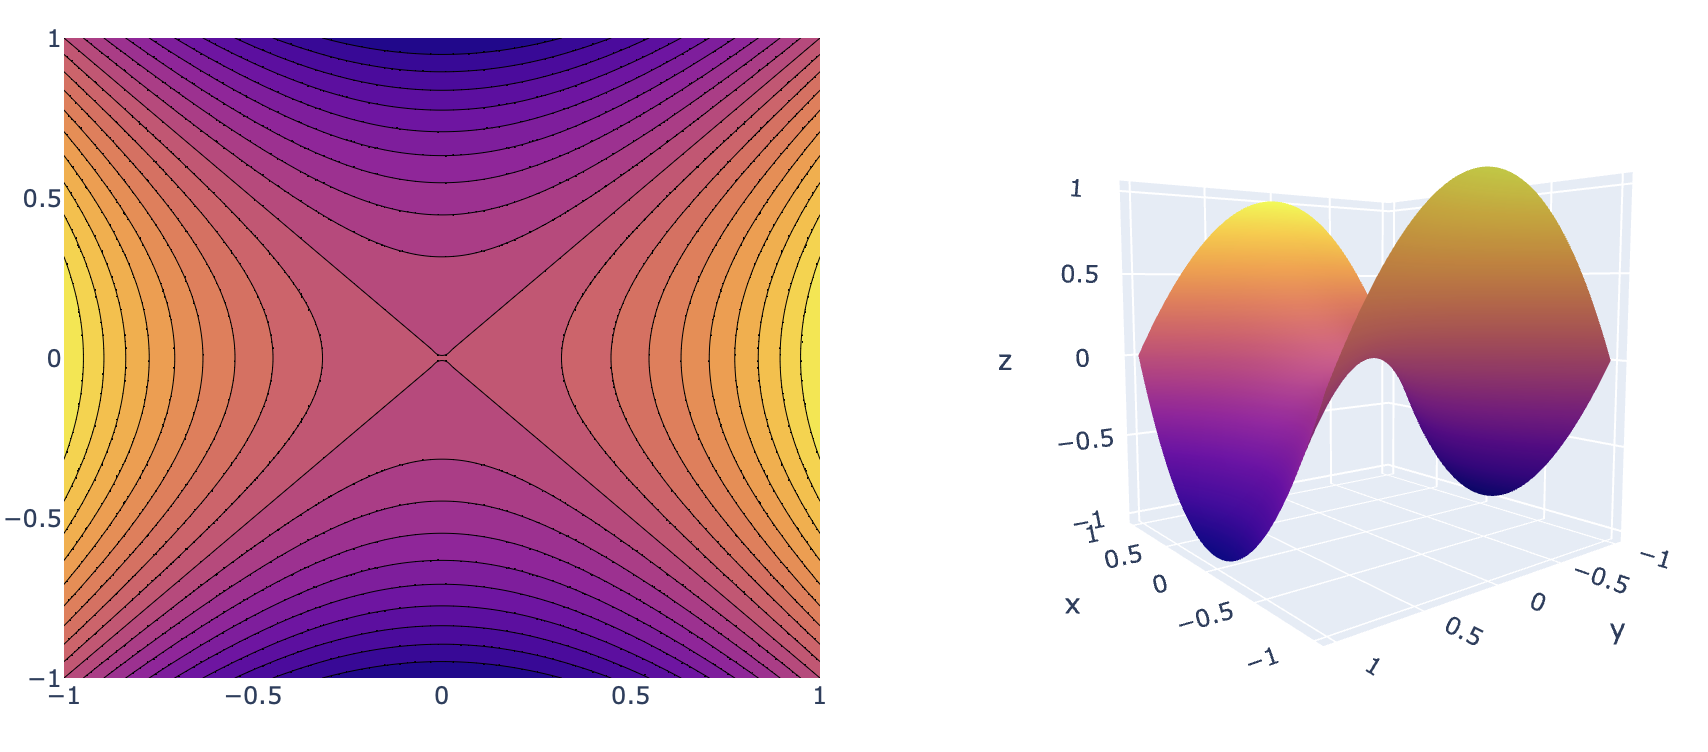
\includegraphics[width=\textwidth]{figures/saddle_point.png}
    \caption{Example of the contours and a 3D surface plot of a saddle point for $\mathbf{x} \in \mathcal{R}^2$.}
    \label{fig:saddle_point}
\end{figure}

One option to find the saddle point is called the \emph{primal method}, where the Lagrangian is first maximized w.r.t. $\pmb{\mu}$ and $\pmb{\lambda}$ with fixed $\mathbf{x}$ and subsequently minimized w.r.t. $\mathbf{x}$. Visually this is a decent along the ridge until we reach the saddle point. 
This formulation 
\begin{equation}
    \min_{\mathbf{x} \in \mathcal{X}} \underbrace{\max_{\pmb{\mu},\pmb{\lambda}} \mathcal{\mathcal{L}}(\pmb{\mu}, \pmb{\lambda}, \mathbf{x})}_{\bar{\mathcal{\mathcal{L}}}(\mathbf{x})}
\end{equation}
does not provide any helpful improvement, because the inner term $\bar{\mathcal{\mathcal{L}}}(\mathbf{x})$ just states the constraints 
\begin{align}
    \frac{\partial \mathcal{\mathcal{L}}}{\partial \mu_i} &= g_i(\mathbf{x}) = 0 \quad i \in \mathcal{I}\\
    \frac{\partial \mathcal{\mathcal{L}}}{\partial \lambda_j} &= h_j(\mathbf{x}) = 0 \quad j \in [1,m]
\end{align}
with $\mathcal{I}$ denoting the set of active inequality constraints. This leaves us with the same problem as \eqref{eq:constrained_optimization} and not much has been gained. 

However, it can be proven that for convex problems with linearly independent inequality constraints, we can invert the process and minimize the Lagrangian function w.r.t. $\mathbf{x}$ first and then maximize it w.r.t. $\pmb{\mu}$ and $\pmb{\lambda}$. Visually this is a maximization along the valley floor until we reach the saddle point \cite{Harzheim2014}. The formulation 
\begin{equation}
     \max_{\pmb{\mu},\pmb{\lambda}} \underbrace{\min_{\mathbf{x}\in \mathcal{X}} \mathcal{\mathcal{L}}(\pmb{\mu}, \pmb{\lambda}, \mathbf{x})}_{\underline{\mathcal{\mathcal{L}}} (\pmb{\mu}, \pmb{\lambda})}
\end{equation}
is helpful, because we are left with very simple box constraints in these optimization problems ($\mathbf{x} \in \mathcal{X}$ in the inner minimization and $\pmb{\mu} \ge 0$ in the maximization). 

\begin{example}{Dual problem}{dualityexample}
    We want to find the solution of the following quadratic optimization problem for $\mathbf{x} \in \mathcal{R}^2$
    \begin{equation}
        \begin{aligned}
            \min_{\mathbf{x}} \quad & f(\mathbf{x})= (\mathbf{x}-\tilde{\mathbf{x}}) \cdot \mathbf{Q} \cdot (\mathbf{x}-\tilde{\mathbf{x}})\\
            \textrm{s.t.} \quad     & h(\mathbf{x}) = (x_1+1)^2 + x_2 = 0  \\
        \end{aligned}
    \end{equation}
    with 
    \begin{equation}
        \mathbf{Q} = 
        \begin{pmatrix}
        2 & 0 \\
        0 & 1 
        \end{pmatrix} 
        \quad 
        \text{and}
        \quad
        \tilde{\mathbf{x}} = 
        \begin{pmatrix}
        -1\\
        1 
        \end{pmatrix}.
    \end{equation}

    This is visually equivalent to searching for a point on the black line in the following image that has the smallest function value.
    \begin{center}
        \includesvg[width=0.5\textwidth]{figures/dual_example.svg}
    \end{center}

    We can formulate the Lagrangian function as
    \begin{equation}
        \mathcal{\mathcal{L}}(\mathbf{x}, \lambda) = 2 (x_1-\tilde{x}_1)^2 + (x_2-\tilde{x}_2)^2 + \lambda \left[(x_1+1)^2 + x_2 \right].
    \end{equation}
    Now, we solve the dual problem by first minimizing the Lagrange function w.r.t. $\mathbf{x}$. For the stationary point, 
    \begin{align}
        \frac{\partial \mathcal{L}}{\partial x_1} &= 4 x^*_1 +4 + 2 \lambda x^*_1 + 2 \lambda = 0\\
        \frac{\partial \mathcal{L}}{\partial x_2} &= 2 x^*_2 - 2 + \lambda = 0
    \end{align} 
    applies. Hence, we can substitute 
    \begin{align}
        x^*_1(\lambda) = -1 \\
        x^*_2(\lambda) = 1 - \frac{1}{2} \lambda 
    \end{align}
    in $\mathcal{L}$ to obtain the dual objective function $\underline{\mathcal{L}} (\lambda)$. Now, we are left with a problem 
    \begin{equation}
        \max_{\lambda} \underline{\mathcal{L}} (\lambda) = 
        \max_{\lambda} \left( - \frac{\lambda^2}{4} + \lambda + \frac{1}{4} \right).
    \end{equation}
    The maximum is located at a stationary point, so with 
    \begin{equation}
        \frac{\partial \underline{\mathcal{L}} }{\partial \lambda} = 1 - \frac{\lambda^*}{2}  = 0
    \end{equation}
    we get $\lambda^*=2$, $x_1^*=-1$ and $x_2^*=0$.
\end{example}

The example shows that we need to be able to express the design variables $\mathbf{x}$ in terms of the Lagrangian variables in order to apply the dual method. This is typically not applicable to general optimization problems. However, the dual method is very attractive for \emph{separable} convex optimization problems, i.e. if the objective function can be expressed as 
\begin{equation}
    f(\mathbf{x}) = f_0 + \sum_{k=1}^d f_k(x_k)
\end{equation}
and the constraints can be expressed as 
\begin{align}
    g_i(\mathbf{x}) & = g_{i0} + \sum_{k=1}^d g_{ik}(x_k) \quad i \in [1,n]\\
    h_j(\mathbf{x}) & = h_{j0} + \sum_{k=1}^d h_{jk}(x_k) \quad j \in [1,m].
\end{align}
Then, the Lagrangian becomes 
\begin{equation}
    \mathcal{L} (\mathbf{x}, \pmb{\mu}, \pmb{\lambda}) = f_0 + \sum_{k=1}^d f_i(x_k) + \sum_{i=1}^n \mu_i \left(g_{i0} + \sum_{k=1}^d g_{ik}(x_k) \right) + \sum_{j=1}^m \lambda_j  \left(h_{j0} + \sum_{k=1}^d h_{jk}(x_k) \right)
\end{equation}
and is also separable
\begin{equation}
    \mathcal{L} (\mathbf{x}, \pmb{\mu}, \pmb{\lambda}) = \mathcal{L}_0 + \sum_{k=1}^d \mathcal{L}_k(x_k)
\end{equation}
with 
\begin{align}
    \mathcal{L}_0 &= f_0 + \sum_{i=1}^n \mu_i g_{i0} + \sum_{j=1}^m \lambda_j  h_{j0} \\
    \mathcal{L}_k (x_k) & = f_k(x_k) + \sum_{i=1}^n \mu_i g_{ik}(x_k) + \sum_{j=1}^m \lambda_j  h_{jk}(x_k). 
\end{align}
For such a separable convex problem, the search for the the "valley floor" 
\begin{equation}
    \min_{\mathbf{x}\in \mathcal{X}} \mathcal{L}(\pmb{\mu}, \pmb{\lambda}, \mathbf{x})
\end{equation} 
turns into $d$ simple strictly convex optimization problems 
\begin{equation}
    \min_{x_k \in [x_k^l, x_k^u]} \mathcal{L}_k(x_k) \quad k \in[1,d]
\end{equation}
which have a unique solution and are simple to solve because each of them is just a box-constrained single variable optimization problem. 
After finding the expression for $\underline{\mathcal{L}} (\pmb{\mu}, \pmb{\lambda})$ easily, we only need to solve this remaining problem $\max_{\pmb{\mu}, \pmb{\lambda}} \underline{\mathcal{L}} (\pmb{\mu}, \pmb{\lambda})$ w.r.t. $\pmb{\mu}$ and $\pmb{\lambda}$. The dual problem is therefore especially well suited for separable convex problems with $d \gg n+m$, i.e. for problems with many design variables and just a few constraints. This is typically the case for topology optimization.

\begin{example}{Separable problem}{separableexample}
    Let's consider the previous example with the additional constraint $\mathbf{x} \in \mathcal{X} = [0, 2]\times[-2, 2]$.
    This is visually equivalent to searching within the gray box for a point on the black line that has the smallest function value in the following image.
    \begin{center}
        \includesvg[width=0.5\textwidth]{figures/separable_example.svg}
    \end{center}

    It would be tedious to solve the problem with additional inequality constraints like $g_1= x_1, g_2=x_1-2, g_3=x_2-2, g_4=2-x_2$. 

    However, we can formulate a separable Lagrangian function as
    \begin{equation}
        \mathcal{L}(\mathbf{x}, \lambda) = \underbrace{2 (x_1-\tilde{x}_1)^2 + \lambda (x_1+1)^2}_{\mathcal{L}_1(x_1)} + \underbrace{(x_2-\tilde{x}_2)^2  + \lambda x_2}_{\mathcal{L}_2(x_2)}.
    \end{equation}
    and can take care of box constraints trivially in each optimization by clipping. Using the stationary points 
    \begin{align}
        \frac{\partial \mathcal{L}_1}{\partial x_1} &= 4\hat{x}_1+4+2\lambda \hat{x}_1 + 2 \lambda = 0 \\
        \frac{\partial \mathcal{L}_2}{\partial x_2} &= 2\hat{x}_2-2+\lambda = 0
    \end{align}
    we can solve 
    \begin{align}
        x_1^*(\lambda) = \max(\min(\hat{x}_1(\lambda), x_1^u), x_1^l) &= 0 \\
        x_2^*(\lambda) = \max(\min(\hat{x}_2(\lambda), x_2^u), x_2^l) &= 
        \begin{cases}
            2 & \quad \lambda < -2 \\
            -2 & \quad \lambda > 6 \\
            1 - \frac{\lambda}{2} & \quad \text{else}
        \end{cases}
    \end{align}
    and the dual objective function becomes 
    \begin{equation}
        \underline{\mathcal{L}}(\lambda) = 
        \begin{cases}
            3 + 3 \lambda  & \quad \lambda < -2 \\
            11 - \lambda  & \quad \lambda > 6 \\
            2 + 2 \lambda - \frac{\lambda^2}{4}   & \quad \text{else.}
        \end{cases}
    \end{equation}
    This dual objective function is plotted here:
    \begin{center}
        \includesvg[width=\textwidth]{figures/dual_function.svg}
    \end{center}
    We can employ any gradient decent method or analytical method to find the optimum of the dual function. In this case, it is $\lambda^*=4$ and therefore the optimum is at $x_1^*=0$ and $x_2^*=-1$.    
\end{example}

\bibliographystyle{unsrtnat}
\bibliography{literature} 
\chapter{Optimization using local approximations}
The optimization problems in the previous chapters utilized explicit functions for the objective functions and constraints. However, in most practical structural optimization problems, we are not able to formulate such explicit functions. Instead, we use local approximations as a remedy. These should be explicit convex functions that approximate the structural problem in a local region well and are easy to solve at the same time. 

The procedure using a local approximation is as follows:

\begin{enumerate}
    \item Choose a starting point $\mathbf{x}^0$
    \item Evaluate the target function, constraints and their gradients at the current position $\mathbf{x}^k$.
    \item Construct a local, explicit, and convex approximation $\tilde{f}, \tilde{g}, \tilde{h}$ at $\mathbf{x}^k$.
    \item Solve the approximated optimization problem to find the next point $\mathbf{x}^{k+1}$. 
    \item Repeat steps 2, 3, and 4 until you reached a maximum number of iteration $k \le N$ or there is no improvement anymore.
\end{enumerate}

Note that during the optimization within each iteration, we use only the approximation and do not have to evaluate the expensive target function.

\begin{objectives}{}{objectives_approximation}
After studying this chapter and finishing the exercise, you should be able to 
\begin{itemize}[label=$\dots$]
    \item approximate an optimization problem via Sequential Linear Programming (SLP)
    \item approximate an optimization problem via Sequential Quadratic Programming (SQP)
    \item approximate an optimization problem via Convex Linearization (CONLIN)
    \item approximate an optimization problem via the Method of Moving Asymptotes (MMA)
    \item discuss the relation between these approximation methods and chose an appropriate method for a given task
\end{itemize}
\end{objectives}

\section{Sequential linear programming}
In Sequential Linear Programming (SLP), we approximate the functions in Equation \eqref{eq:constrained_optimization} at $\mathbf{x}^k$ with first order linear equations  
\begin{align}
    \tilde{f}(\mathbf{x}) &= f(\mathbf{x}^k) + \nabla f(\mathbf{x}^k) \cdot \left(\mathbf{x} - \mathbf{x}^k \right) \\
    \tilde{g}_i(\mathbf{x}) &= g_i(\mathbf{x}^k) + \nabla g_i(\mathbf{x}^k) \cdot \left(\mathbf{x} - \mathbf{x}^k \right) \\
    \tilde{h}_j(\mathbf{x}) &= h_j(\mathbf{x}^k) + \nabla h_j(\mathbf{x}^k) \cdot \left(\mathbf{x} - \mathbf{x}^k \right)
\end{align}
and limit the validity of the approximation with so-called \emph{move limits} 
\begin{equation}
    \tilde{\mathbf{x}}^{-,k} \le \mathbf{x} \le \tilde{\mathbf{x}}^{+,k}.
\end{equation}
The resulting functions are explicit linear expressions and the set for $\mathbf{x}$ is compact, hence the resulting problem is strictly convex. We limit the set because i) the approximation is only valid close to $\mathbf{x}^k$ and ii) the linear problem requires a compact set to be strictly convex. 

\begin{example}{SLP with move limits}{slpexample}
    We want to sequentially approximate the following quadratic function
    \begin{equation}
             f(\mathbf{x})= \mathbf{x} \cdot \mathbf{Q} \cdot \mathbf{x} \quad \text{with} \quad \mathbf{x} \in \mathcal{R}^2 \quad \text{and} \quad 
             \mathbf{Q} = 
            \begin{pmatrix}
            2 & 1 \\
            1 & 1 
            \end{pmatrix}. 
    \end{equation}
    Obviously, this is already an explicit convex function and we do not necessarily need to employ an approximation to minimize a function like this. But for the sake of this example, we assume that $f(\mathbf{x})$ is a very complex function with no explicit expression. 
    
    In this case we can get an explicit linear approximation
    \begin{align}
        \tilde{f}(\mathbf{x}) = f(\mathbf{x}^k) + 2(\mathbf{Q} \cdot \mathbf{x}^k) \cdot \left(\mathbf{x} - \mathbf{x}^k \right)
    \end{align}
    with an analytical expression for the gradient. Then, a first approximation at $\mathbf{x}^0=(1,1)^\top$ is 
    \begin{equation}
        \tilde{f}(\mathbf{x}) = 3 + \begin{pmatrix} 2\\1 \end{pmatrix} \cdot \left(\mathbf{x} - \mathbf{x}^k \right).
    \end{equation}
    Assuming a validity of $\pm 0.5$ around the approximated point, the move limits are $\tilde{\mathbf{x}}^{-,0}=(0.5, 0.5)^\top$ and  $\tilde{\mathbf{x}}^{+,0}=(1.5, 1.5)^\top$.  
    An optimization with these conditions yields to the next point $\mathbf{x}^1=(0.5,0.5)^\top$ with 
    \begin{equation}
        \tilde{f}(\mathbf{x}) = 1.25 + \begin{pmatrix} 1\\0.5 \end{pmatrix} \cdot \left(\mathbf{x} - \mathbf{x}^k \right)
    \end{equation}
    and with move limits $\tilde{\mathbf{x}}^{-,1}=(0, 0)^\top$ and  $\tilde{\mathbf{x}}^{+,1}=(1, 1)^\top$. 
    An optimization under these conditions gives us the final result $(0,0)^\top$ for the minimum of the function $f(\mathbf{x})$. We obtained this by sequentially employing linear approximations and then performing optimization on these approximations instead of the original "complex" and expensive function.
\end{example}

\section{Sequential quadratic programming}
In Sequential Quadratic Programming (SQP), we approximate the objective function in Equation \eqref{eq:constrained_optimization} at $\mathbf{x}^k$ with second order quadratic equations  
\begin{equation}
    \tilde{f}(\mathbf{x}) = f(\mathbf{x}^k) + \nabla f (\mathbf{x}^k) \cdot \left(\mathbf{x} - \mathbf{x}^k \right) + \left(\mathbf{x} - \mathbf{x}^k \right) \cdot \nabla^2 f(\mathbf{x}^k) \cdot \left(\mathbf{x} - \mathbf{x}^k \right)
\end{equation}
and the restrictions with first order linear approximations
\begin{align}
    \tilde{g}(\mathbf{x}) &= g(\mathbf{x}^k) + \nabla g(\mathbf{x}^k) \left(\mathbf{x} - \mathbf{x}^k \right) \\
    \tilde{h}(\mathbf{x}) &= h(\mathbf{x}^k) + \nabla h(\mathbf{x}^k) \left(\mathbf{x} - \mathbf{x}^k \right).
\end{align}
This results in a more accurate approximation and also in a more balanced approximation, i.e. the same approximation order for the roots of interest (for constraints we are interested in roots of the function itself, for the objective we are interest in the roots of the derivative). 
The Hessian $\nabla^2 f$ may be approximated efficiently using the BFGS algorithm. This way, the problem is convex and we may use the methods from Chapter 3 to obtain the optimum. 

\section{Convex linearization}
Both, SLP and SQP, can be applied for any non-linear optimization problem. However, we can improve the approximation quality significantly, if we leverage some knowledge about the fundamental equation types seen in structural optimization.

Let's consider an assembly of beams and design variables that describe the cross sectional areas of the beams like in the last example of Exercise 3. A property like volume or mass is linearly related to the design variables and a linear approximation would be exact. Conversely, stress and displacement are related to the inverse of the design variable and we would need many sequential linear approximations to approximate the inverse.  However, this knowledge suggests that it would be clever to substitute $y_j = x^{-1}_j$, which would lead to a exact approximations for statically determined truss assemblies \cite{Christensen2008}. 
%The notation $\bullet_j$ is used here for element-wise operations, i.e. double indices of this type do not imply a summation according to Einstein's summation convention. 
Then, our linear approximation becomes 
\begin{equation}
    \tilde{f}(\mathbf{x}) = f(\mathbf{x}^k) + \sum_j \frac{\partial f}{\partial y_j}(\mathbf{x}^k) \left(y_j(x_j) - y_j(x^k_j) \right)
\end{equation}
for the objective function, but obviously the same principles apply for constraints throughout the remainder of this chapter.
Employing the chain rule
\begin{equation}
    \frac{\partial f}{\partial y_j} (\mathbf{x}^k) 
    = \frac{\partial x_j}{\partial y_j}(\mathbf{x}^k) \frac{\partial f}{\partial x_j} (\mathbf{x}^k)   
    = -(x^k_j)^2 \frac{\partial f}{\partial x_j}(\mathbf{x}^k) 
\end{equation}
this can be simplified to an expression without $y_j$
\begin{equation}
    \tilde{f}(\mathbf{x}) = f(\mathbf{x}^k) + \sum_j \frac{\partial f}{\partial x_j}(\mathbf{x}^k) \underbrace{\frac{x^k_j}{x_j}}_{\Gamma_j} \left(x_j - x^k_j \right). 
\end{equation}
The difference to the regular linear approximation is only the term indicated with $\Gamma_j$. Hence we can set $\Gamma_j = 1$ for variables that should be approximated linearly and set $\Gamma_j = x^k_j / x_j$ for variables that should be approximated inversely. Instead of choosing the approximation for each variable manually, we may use the the sign of the partial derivative and define an approximation method as 
\begin{align}
    \tilde{f}(\mathbf{x}) &= f(\mathbf{x}^k) + \sum_j \frac{\partial f}{\partial x_j}(\mathbf{x}^k) \Gamma_j \left(x_j - x^k_j \right) \\
    \Gamma_j &= 
    \begin{cases}
        1 &\quad \text{if} \quad \frac{\partial f}{\partial x_j} (\mathbf{x}^k) \ge 0 \\
        \frac{x^k_j}{x_j} &\quad \text{if} \quad \frac{\partial f}{\partial x_j} (\mathbf{x}^k) < 0.
    \end{cases}
\end{align}
This method is termed \emph{Convex Linearization} or CONLIN \cite{Fleury1989}. The CONLIN method provides a convex separable optimization problem, hence the Lagrangian duality method is a suitable solution method  \cite{Christensen2008,Harzheim2014}.

\begin{example}{CONLIN}{conlinexample}
    The volume of a four-bar truss \cite{Christensen2008} should be minimized under the displacement constraint $\delta \le \delta_0$. There is a force $P>0$ and all bars have identical lengths $l$ and identical Young's moduli $E$. The modifiable structural variables are the cross sectional areas $A_1=A_4$ and $A_2=A_3$. We define $A_0 = Pl / (10\delta_0E)$ and constrain the variables $0.2A_0 \le A_j \le 2.5 A_0$. Then we can use dimensionless design variables $a_1=A_1/A_0 \in [0.2, 2.5]$ and $a_2=A_2/A_0 \in [0.2, 2.5]$.
    \begin{center}
        
\includegraphics[width=0.8\textwidth]{figures/four_bar_truss_transparent.png}
    \end{center}
    The optimization problem is 
    \begin{equation}
        \begin{aligned}
            \min_{\mathbf{a}} \quad & f(\mathbf{a})= a_1 + a_2\\
            \textrm{s.t.} \quad     & g(\mathbf{a}) = \frac{8}{16a_1+9a_2} - \frac{4.5}{9a_1+16a_2} - \delta_0 \le 0  \\
            \quad     & \mathbf{a} \in [0.2,2.5]^2
        \end{aligned}
    \end{equation}
    This problem is not convex, because the constraint $g(\mathbf{a})$ (shown as solid black line in the following plot for $\delta_0=0.1$) is not a convex function. This leads to two local minima, one at $a_2=0.2$ and one at $a_2=2.5$.
    \begin{center}
        \includesvg[width=0.6\textwidth]{figures/four_bar_example_0.svg}
    \end{center}
    
    The CONLIN approximation of the objective function is the objective function itself - it is already linear. A CONLIN approximation of the constraint function at $\mathbf{a}^0=(2,1)^\top$ is computed using automatic differentiation in PyTorch and results in the dashed black line. The resulting problem is convex and can be solved, e.g. using Lagrangian duality. The unique solution of this problem is the point $\mathbf{a}^1=(1.2,0.2)^\top$. We can apply the CONLIN method again at this point to obtain a new convex problem. Solving this problem gives $\mathbf{x}^2=(0.85,0.2)^\top$, which is close to the optimal solution $\mathbf{a}^*$, but could be improved with further iterations. Note that not every CONLIN approximation is conservative, i.e. it can happen that $\tilde{g}(\mathbf{a}) < g(\mathbf{a})$. In that case, the solution will tend to oscillate around the optimal point. 
    \begin{center}
        \includesvg[width=0.6\textwidth]{figures/four_bar_example_1.svg}
    \end{center}
\end{example}

\section{Method of Moving Asymptotes}
CONLIN is an effective method to turn structural optimization problems into convex separable optimization tasks. However, it is sometimes too conservative causing slow convergence or sometimes not conservative enough causing no convergence at all. We could improve the method by adjusting how conservative we approximate a function.

We may obtain an adjustable method by defining
\begin{equation}
    \tilde{f}(\mathbf{x}) = r(\mathbf{x}^k) + \sum_j \left( \frac{p_{j}^k}{U^k_j-x_j} + \frac{q_{j}^k}{x_j-L^k_j} \right) 
    \label{eq:mma_start}
\end{equation}
where
\begin{align}
    p_{j}^k &= 
    \begin{cases}
        (U^k_j-x^k_j)^2 \frac{\partial f}{\partial x_j} (\mathbf{x}^k)  &\quad \text{if} \quad \frac{\partial f}{\partial x_j} (\mathbf{x}^k) > 0 \\
        0 &\quad \text{if} \quad \frac{\partial f}{\partial x_j} (\mathbf{x}^k) \le 0.
    \end{cases} \\ 
    q_{j}^k &= 
    \begin{cases}
         0 &\quad \text{if} \quad \frac{\partial f}{\partial x_j} (\mathbf{x}^k) \ge 0 \\
        - (x^k_j-L^k_j)^2 \frac{\partial f}{\partial x_j} (\mathbf{x}^k) &\quad \text{if} \quad \frac{\partial f}{\partial x_j} (\mathbf{x}^k) < 0.
    \end{cases} \\ 
    r(\mathbf{x}^k) &= f(\mathbf{x}^k) - \sum_j \left(\frac{p_{j}^k}{U^k_j-x^k_j} + \frac{q_{j}^k}{x^k_j-L^k_j}  \right)
    \label{eq:mma_end}
\end{align}
with $L^k_j < x_j < U^k_j$. The parameters $L^k_j$ and $U_j^k$ are called the lower and upper asymptotes, respectively. They can be adjusted ("move"), hence the method is termed \emph{Method of Moving Asymptotes} (MMA) \cite{Svanberg1987}. It can be proven that this is a generalization, as setting $L^k_j \rightarrow 0$ and $U^k_j \rightarrow \infty$ recovers the CONLIN method and setting  $L^k_j \rightarrow -\infty$ and $U^k_j \rightarrow \infty$ recovers the SLP method.

To prevent singularities by reaching the asymptotes, we use move limits 
\begin{equation}
    L^k_j < \tilde{x}_j^{-,k} \le x_j \le \tilde{x}_j^{+,k} < U_j^k.
\end{equation}
similar to SLP. These could be chosen for example as 
\begin{align}
    \tilde{x}_j^{-,k} &= \max(x^-_j,  0.9 L_j^k + 0.1 x_j^k) \\
    \tilde{x}_j^{+,k} &= \min(x^+_j, 0.9 U_j^k + 0.1 x_j^k).
    \label{eq:mma_move_limits}
\end{align}

The advantage of these adjustable asymptotes is that we can bring the asymptotes closer to the current approximation $\mathbf{x}^k$ to obtain a more conservative approximation and move them further away to accelerate convergence speed. But how do we chose the asymptotes? Svanberg \cite{Svanberg1987} suggested the following heuristic approach: 
\begin{enumerate}
    \item In the first two iterations, set 
        \begin{align}
            L_j^k &= x_j^k - s (x^+_j - x^-_j) \\
            U^k_j &= x_j^k + s (x^+_j - x^-_j)
        \end{align}
    with $s \in (0,1)$.
    \item For the following iterations ($k>1$) check for each design variable, if it oscillates. If it oscillates, i.e. $(x_j^k-x_j^{k-1})(x_j^{k-1}-x_j^{k-2}) < 0$, bring asymptotes closer to $x_j^k$ by   
        \begin{align}            
            \label{eq:mma_heuristic_first}
            L_j^k &= x_j^k - s (x_j^{k-1} - L_j^{k-1}) \\
            U_j^k &= x_j^k + s (U_j^{k-1} - x_j^{k-1}).
        \end{align}

    If the solution does not oscillate, i.e. $(x_j^k-x_j^{k-1})(x_j^{k-1}-x_j^{k-2}) \ge 0$, move the asymptotes further away from $x_j^k$ by   
        \begin{align}
            L_j^k &= x_j^k - \frac{1}{\sqrt{s}} (x_j^{k-1} - L_j^{k-1}) \\
            U_j^k &= x_j^k + \frac{1}{\sqrt{s}} (U_j^{k-1} - x_j^{k-1}).
            \label{eq:mma_heuristic_last}
        \end{align}
\end{enumerate}

Svanbergs original version uses the same asymptotes $L_j^k$ and $U_j^k$ for the objective function and constraints. There is also a method termed \emph{Generalized Method of Moving Asymptotes} (GMMA) \cite{Zhang1997} that uses different asymptotes for each function. However, this requires a more complicated heuristic to obtain such asymptotes.

\begin{example}{MMA}{mmaexample}
    Consider the previous example with the optimization problem
    \begin{equation}
        \begin{aligned}
            \min_{\mathbf{a}} \quad & f(\mathbf{a})= a_1 + a_2\\
            \textrm{s.t.} \quad     & g(\mathbf{a}) = \frac{8}{16a_1+9a_2} - \frac{4.5}{9a_1+16a_2} -0.1 \le 0  \\
            \quad     & \mathbf{a} \in [0.2,2.5]^2
        \end{aligned}
    \end{equation}

    A MMA approximation at $\mathbf{a}^0=(2,1)^\top$ is illustrated in the following image with the dashed line for $s_0=0.2$. 
    \begin{center}
        \includesvg[width=0.6\textwidth]{figures/four_bar_example_mma_0.svg}
    \end{center}

    If we chose $s_0=0.5$, we get a less conservative approximation, as shown in the next image. This results in faster convergence, as an optimization of the convex problem gets closer to the optimum in a single step.
    \begin{center}
        \includesvg[width=0.6\textwidth]{figures/four_bar_example_mma_1.svg}
    \end{center}

    This example shows just the first iteration - the full method would require sequential approximation and optimization with the Lagrangian duality method until convergence. During each iteration, we would use the heuristic given in Equations \eqref{eq:mma_heuristic_first} to \eqref{eq:mma_heuristic_last} to update asymptotes.  
\end{example}

\bibliographystyle{unsrtnat}
\bibliography{literature} 
\chapter{Trusses in a nutshell}
After summarizing fundamentals of optimization in previous chapters, we can finally focus on the structural part of \emph{structural optimization}. Hence, we start with fundamentals of discrete truss structures in this chapter and optimize those in the next chapter. 


\begin{objectives}{}{objectives_sizing}
After studying this chapter and finishing the exercise, you should be able to 
\begin{itemize}[label=$\dots$]
    \item explain how general 2D truss problems can be solved employing element stiffness matrices and global stiffness matrices
    \item define your own 2D truss structures and use the accompanying code to solve them
    \item differentiate size, topology, and shape optimization of trusses
\end{itemize}
\end{objectives}

\section{General 2D trusses}
A two-dimensional truss structure is defined by a finite set of $N$ nodes 
\begin{equation}
    \mathcal{N}=\{\mathbf{x}^i \in \mathcal{R}^2, i \in [0, N-1]\}
\end{equation} and a finite set of $M$ element tuples 
\begin{equation}
    \mathcal{E} = \{(\mathbf{x}^0_j, \mathbf{x}^1_j), j \in [0, M-1]\}
\end{equation} 
connecting exactly two nodes $\mathbf{x}^0_j,  \mathbf{x}^1_j \in \mathcal{N}$ each. While $\mathcal{N}$ defines the geometry of a truss, $\mathcal{E}$ defines the topology of a truss. An example of a two-dimensional truss structure with 10 nodes and 20 elements is shown in Figure \ref{fig:truss_example}.

\begin{figure}[!htpb]
    \centering
    \includesvg[width=0.75\textwidth]{figures/truss_sample.svg}
    \caption{Example of a truss with $N=10$ numbered nodes.}
    \label{fig:truss_example}
\end{figure}

In this lecture, all elements transfer only axial forces (positive for tension, negative for compression), have a constant Young's modulus $E$, and have element-wise constant cross sectional areas $\mathbf{a} \in \mathcal{R}^M$. Each node has two degrees of freedom to deform $\mathbf{u}^i \in \mathcal{R}^2$, unless a degree of freedom is constrained by a support. The actual values of $\mathbf{u}^i$ depend on the truss design, i.e. the cross sectional areas or positions of nodes. At each node, there may also act an external force $\mathbf{f}^i \in \mathcal{R}^2$, which is independent of the truss design.

\begin{figure}[!htpb]
    \centering
    \includesvg[width=0.4\textwidth]{figures/single_truss.svg}
    \caption{A single truss element with two nodes.}
    \label{fig:single_truss}
\end{figure}


Without considering optimization for now, we are generally interested in solving the truss problem for the unknown displacements $\mathbf{u}^i$. To do so, we take a look at a single element, like the one shown in Figure \ref{fig:single_truss}. This truss element is defined by two nodes at positions $\mathbf{x}^0_j$ and $\mathbf{x}^1_j$. It has four degrees of freedom 
\begin{equation}
    \mathbf{u}_j = 
    \begin{pmatrix}
        \mathbf{u}^0_j \\  \mathbf{u}^1_j
    \end{pmatrix}
    = 
    \begin{pmatrix}
        (u_1)^0_j \\ (u_2)^0_j \\  (u_1)^1_j \\ (u_2)^1_j
    \end{pmatrix}
\end{equation} 
and four nodal forces 
\begin{equation}
    \mathbf{f}_j = 
    \begin{pmatrix}
        \mathbf{f}^0_j \\  \mathbf{f}^1_j
    \end{pmatrix}
    = 
    \begin{pmatrix}
        (f_1)^0_j\\ (f_2)^0_j\\ (f_1)^1_j \\ (f_2)^1_j
    \end{pmatrix},
\end{equation} 
where $\mathbf{u}_j \in \mathcal{R}^4$ and $\mathbf{f}_j \in \mathcal{R}^4$. 
The displacements can be related to the nodal forces via 
\begin{equation}
    \mathbf{f}_j = \mathbf{k}_j \cdot \mathbf{u}_j
    \label{eq:local_truss_stiffness}
\end{equation}
with an element stiffness matrix $\mathbf{k}_j \in \mathcal{R}^{4\times4}$ defined as \cite{Christensen2008}
\begin{equation}
    \mathbf{k}_j = \frac{a_j E}{l_j}
    \begin{pmatrix}
    \cos{\phi}^2 & \cos{\phi}\sin{\phi} & -\cos{\phi}^2 & -\cos{\phi}\sin{\phi} \\
    \cos{\phi}\sin{\phi} & \sin{\phi}^2 & -\cos{\phi}\sin{\phi} & -\sin{\phi}^2 \\
    -\cos{\phi}^2 & \cos{\phi}\sin{\phi} & \cos{\phi}^2 &\cos{\phi}\sin{\phi} \\
    -\cos{\phi}\sin{\phi} & -\sin{\phi}^2 & \cos{\phi}\sin{\phi} & \sin{\phi}^2 \\
    \end{pmatrix}
\end{equation}
using the orientation angle of the element $\phi = \arctan\left(\frac{x^0_2-x^1_2}{x^0_1-x^1_1}\right)$, the cross sectional area of an element $a_j$, and the length 
\begin{equation}
    l_j = \sqrt{(x^0_2-x^1_2)^2 + (x^0_1-x^1_1)^2}.
\end{equation}
This element stiffness matrix is symmetric and positive semi-definite, i.e. \begin{equation}
    \mathbf{v} \cdot \mathbf{k}_j \cdot \mathbf{v} \ge 0 \hspace{0.5em} \forall \mathbf{v}.
\end{equation}

Similar to the local relation in Equation \eqref{eq:local_truss_stiffness}, we can denote a global relation for all degrees of freedom $\mathbf{u} \in \mathcal{R}^{2N}$ and all forces $\mathbf{f} \in \mathcal{R}^{2N}$ as 
\begin{equation}
    \mathbf{f} = \mathbf{K} \cdot  \mathbf{u} 
    \label{eq:global_stiffness}
\end{equation}
with a global stiffness matrix $\mathbf{K} \in \mathcal{R}^{2N \times 2N}$. This global stiffness matrix is \emph{assembled} from element stiffness matrices by adding entries of all element stiffness matrices at the correct positions. This can be written as 
\begin{equation}
    \underbrace{
    \begin{pmatrix}
        \dots \\ (f_1)^0_j \\ (f_2)^0_j \\ \dots \\ (f_1)^1_j \\ (f_2)^1_j \\ \dots \\
    \end{pmatrix}}_{\mathbf{f}}
    =
    \underbrace{
    \sum_j
    \underbrace{
    \begin{pmatrix}
    \dots & \dots & \dots & \dots & \dots & \dots & \dots \\
    \dots & (k_{11})_j & (k_{12})_j & \dots & (k_{13})_j & (k_{14})_j & \dots  \\
    \dots & (k_{21})_j & (k_{22})_j & \dots & (k_{23})_j & (k_{24})_j & \dots  \\
    \dots & \dots & \dots & \dots & \dots & \dots & \dots  \\
    \dots & (k_{31})_j & (k_{32})_j & \dots & (k_{33})_j & (k_{34})_j & \dots  \\
    \dots & (k_{41})_j & (k_{42})_j & \dots & (k_{43})_j & (k_{44})_j & \dots  \\
    \dots & \dots & \dots & \dots & \dots & \dots & \dots  \\
    \end{pmatrix}}_{\mathbf{K}_j}
    }_{\mathbf{K}}
    \underbrace{
    \begin{pmatrix}
        \dots \\ (u_1)^0_j \\ (u_2)^0_j \\ \dots \\ (u_1)^1_j \\ (u_2)^1_j \\ \dots \\
    \end{pmatrix}}_{\mathbf{u} (\mathbf{a})},
\end{equation}
where the degrees of freedom $(u_1)^0_j, (u_2)^0_j$ etc. are at the positions in the vector corresponding to the global node displacements $\mathbf{u}$. The matrices $\mathbf{K}_j$ are zero everywhere except for the 16 positions at which they are filled with values from $\mathbf{k}_j$.
The global stiffness matrix is symmetric and positive semi-definite, just like the element stiffness matrix.

Before solving the global system of equations, we need to remove those entries containing constrained degrees of freedom. This is achieved by simply removing all constrained entries in $\mathbf{f}$ and $\mathbf{u}$ and the corresponding rows and columns in the global stiffness matrix $\mathbf{K}$. If we do not remove sufficient degrees of freedom, the matrix would be singular and cannot be solved. The physical interpretation of this behavior is simple: The truss would be statically undetermined and can experience rigid body motions.

Finally, after removing constraints, we end up with a reduced system of equations 
\begin{equation}
     \mathbf{f}_\textrm{red} = \mathbf{K}_\textrm{red}  \cdot \mathbf{u}_\textrm{red} 
     \label{eq:reduced_system}
\end{equation}
where $\mathbf{K}_\textrm{red}$ is strictly positive definite and not singular (if sufficient boundary conditions have been applied). Solving this system of equation gives us the unknown node displacements $\mathbf{u}$. 

\begin{figure}[!htpb]
    \centering
    \includesvg[width=\textwidth]{figures/truss_sample_solved.svg}
    \caption{Exemplary solution of a truss computation for the example shown in Figure \ref{fig:truss_example}.}
    \label{fig:truss_example_solved}
\end{figure}

As a post-processing step, we may compute the stress in each element via
\begin{equation}
    S_j = \frac{E}{l_j} 
    \begin{pmatrix}
        \cos{\phi} & \sin{\phi} & -\cos{\phi} & -\sin{\phi}
    \end{pmatrix}
    \cdot 
    \mathbf{u}_j.
\end{equation}

An exemplary solution for the example shown in Figure \ref{fig:truss_example} is given in Figure \ref{fig:truss_example_solved} with colors indicating the stresses in trusses.

\begin{example}{Three bar truss}{trussexample}
    Consider the truss shown below, which is subjected to a force $P$ indicated by the gray arrow and supports indicated by gray triangles. It has three nodes 
    \begin{equation}
        \mathcal{N} = \{\mathbf{x}^0=(1,0)^\top, \mathbf{x}^1=(0,0)^\top,\mathbf{x}^2=(0,1)^\top \}
    \end{equation}
    and three elements 
    \begin{equation}
        \mathcal{E} = \{(\mathbf{x}^0, \mathbf{x}^1), (\mathbf{x}^0, \mathbf{x}^2), (\mathbf{x}^1, \mathbf{x}^2)\}.
    \end{equation}

    \begin{center}
        \includesvg[width=0.5\textwidth]{figures/three_bar_truss.svg}
    \end{center}

    The element stiffness matrices in local coordinates are 
    \begin{equation}
        \mathbf{k}_0 = E a_0
        \begin{pmatrix}
             1 & 0 & -1 & 0 \\
             0 & 0 &  0 & 0 \\
            -1 & 0 &  1 & 0 \\
             0 & 0 &  0 & 0
        \end{pmatrix},
    \end{equation}
    \begin{equation}
        \mathbf{k}_1 = \frac{E a_1}{2\sqrt{2}}
        \begin{pmatrix}
             1 & -1 & -1 &  1 \\
            -1 &  1 &  1 & -1 \\
            -1 &  1 &  1 & -1 \\
             1 & -1 & -1 &  1
        \end{pmatrix}
    \end{equation}
    and 
    \begin{equation}
        \mathbf{k}_2 = E a_2
        \begin{pmatrix}
            0 &  0 & 0 &  0 \\
            0 &  1 & 0 & -1 \\
            0 &  0 & 0 &  0 \\
            0 & -1 & 0 &  1 
        \end{pmatrix}.
    \end{equation}

    The global stiffness matrix is 
    \begin{equation}
        \mathbf{K} = E
        \begin{pmatrix}
             a_0 + \frac{a_1}{2\sqrt{2}}&  -\frac{a_1}{2\sqrt{2}} & \cellcolor{aux_green!10}-a_0 &  \cellcolor{aux_green!10}0 & -\cellcolor{aux_green!10} \frac{a_1}{2\sqrt{2}} &  \frac{a_1}{2\sqrt{2}}\\
            -\frac{a_1}{2\sqrt{2}} &  \frac{a_1}{2\sqrt{2}} & \cellcolor{aux_green!10} 0 & \cellcolor{aux_green!10} 0 & \cellcolor{aux_green!10}\frac{a_1}{2\sqrt{2}} &  -\frac{a_1}{2\sqrt{2}} \\
            \rowcolor{aux_green!10}
             -a_0 &  a_0 & 0 &  0 & 0 & 0\\
             \rowcolor{aux_green!10}
            0 &  0 & 0 &  a_2 & 0 &  -a_2 \\
            \rowcolor{aux_green!10}
             -\frac{a_1}{2\sqrt{2}} &  \frac{a_1}{2\sqrt{2}} & 0 &  0 & \frac{a_1}{2\sqrt{2}} &  -\frac{a_1}{2\sqrt{2}}\\
            \frac{a_1}{2\sqrt{2}} &  -\frac{a_1}{2\sqrt{2}} & \cellcolor{aux_green!10} 0 &  \cellcolor{aux_green!10} -a_2 & \cellcolor{aux_green!10} -\frac{a_1}{2\sqrt{2}} &  a_2 + \frac{a_1}{2\sqrt{2}}\\
        \end{pmatrix}
    \end{equation}
    with colored rows and columns indicating those entries which will be removed due to constraints. This leads to the reduced system 
    \begin{equation}
        \begin{pmatrix}
            0 \\ -P \\ 0  \\
        \end{pmatrix}
         = E
        \begin{pmatrix}
             a_0 + \frac{a_1}{2\sqrt{2}}&  -\frac{a_1}{2\sqrt{2}} &  \frac{a_1}{2\sqrt{2}}\\
            -\frac{a_1}{2\sqrt{2}} &  \frac{a_1}{2\sqrt{2}} &  -\frac{a_1}{2\sqrt{2}} \\
            \frac{a_1}{2\sqrt{2}} &  -\frac{a_1}{2\sqrt{2}} &  a_2 + \frac{a_1}{2\sqrt{2}}
        \end{pmatrix}
        \mathbf{u}_\textrm{red}
    \end{equation}
    which can be solved for 
    \begin{equation}
        \mathbf{u}_\textrm{red} = 
        \begin{pmatrix}
            -\frac{P}{Ea_0} \\  \frac{2\sqrt{2}P}{Ea_2} - \frac{P}{Ea_0} - \frac{P}{Ea_1} \\ -\frac{P}{Ea_1}  \\
        \end{pmatrix}
    \end{equation}

    The final result of the computation is shown below.
    
    \begin{center}
        \includesvg[width=0.5\textwidth]{figures/three_bar_truss_solved.svg}
    \end{center}    
\end{example}

\section{Optimization types for trusses}
Truss structures may be optimized by size optimization, topology optimization and shape optimization: 
\begin{description}
    \item[Size:]{In size optimization, we seek the optimal truss cross section areas $\mathbf{a}$ for fixed node positions $\mathbf{x}$ and a fixed topology, i.e. fixed connections $\mathcal{E}$. An example for this is shown in Figure \ref{fig:bridge_size}.} 
    \item[Topology:]{In topology optimization, we want find the optimal connections in a truss $\mathcal{E}$ with cross sectional areas being either the maximum or minimum value for fixed node positions $\mathbf{x}$. An example for this is shown in Figure \ref{fig:bridge_topology}.}
    \item[Shape:]{In shape optimization, we want to find the optimal positions of nodes $\mathbf{x}$ in a truss for fixed cross sectional areas $\mathbf{a}$ and a fixed topology $\mathcal{E}$.}
\end{description}

\begin{figure}[!ht]
    \centering
    \includesvg[width=\textwidth]{figures/bridge_size_optimized.svg}
    \caption{Bridge truss size optimization}
    \label{fig:bridge_size}
\end{figure}

\begin{figure}[!ht]
    \centering
    \includesvg[width=\textwidth]{figures/bridge_topology_optimized.svg}
    \caption{Bridge truss topology optimization}
    \label{fig:bridge_topology}
\end{figure}

\begin{figure}[!ht]
    \centering
    \includesvg[width=\textwidth]{figures/bridge_shape_optimized.svg}
    \caption{Bridge truss shape optimization}
    \label{fig:bridge_shape}
\end{figure}




\bibliographystyle{unsrtnat}
\bibliography{literature} 
\chapter{Optimization of truss structures}
In this chapter, we focus on the optimization of discrete truss structures. A general procedure to solve such problems involves the following steps:
\begin{enumerate}
    \item Definition of the truss with all nodes, elements, material properties, constraints and initial design choice
    \item Solution of unknown displacements for each node in the truss given the current design
    \item Evaluation of the objective function and its gradients w.r.t. the design variables
    \item Approximation of the problem with MMA at the current design point
    \item Solution of the approximated dual problem to find the next design point
    \item Repetition of steps 2,3,4 and 5 until a maximum of iterations is reached or until there is no improvement of the objective function any more
\end{enumerate}


\begin{objectives}{}{objectives_shape}
After studying this chapter and finishing the exercise, you should be able to 
\begin{itemize}[label=$\dots$]
    \item define optimization problems to minimize compliance of two-dimensional trusses with a volume constraint
    \item explain properties of the aforementioned optimization problem
    \item employ MMA to solve two-dimensional truss optimization problems
\end{itemize}
\end{objectives}

\section{Size Optimization}
One possible objective in truss optimization is the search for the cross sectional areas $\mathbf{a}$ resulting in the stiffest truss. The corresponding objective function could be simply the displacement at a specific node or a global displacement measure $\mathbf{u} (\mathbf{a}) \cdot \mathbf{u} (\mathbf{a})$. However, we choose to minimize the compliance $C: \mathcal{R}^{M} \rightarrow \mathcal{R}$ defined as 
\begin{equation}
    C(\mathbf{a}) = \mathbf{f} \cdot \mathbf{u}(\mathbf{a})
\end{equation} 
of the truss instead. The minimal compliance results also in the stiffest truss, but this formulation is preferred over the pure displacement formulation, because $C(\mathbf{a})$ is convex \cite{Svanberg1984}. The convexity is proven by showing that the Hessian $\nabla^2 C(\mathbf{a})$ is positive semi-definite, a property that is inherited from the positive semi-definiteness of $\mathbf{K}(\mathbf{a})$ (see Chapter 5.2.1 in \cite{Christensen2008} for details).

We employ box constraints $\mathcal{A}$ on the upper and lower limit of the design variables. The upper limit $\mathbf{a}^u$ could be a manufacturing constraint that prevents very thick elements. The lower limit $\mathbf{a}^l$ should be larger than $0$ to prevent deletion of truss elements. If the cross sectional area of all elements connected to a node would become $0$, i.e. all trusses are deleted, the displacement of that node would be undetermined and the stiffness matrix would become singular. In this chapter, we prevent this by demanding $a_j^l > 0$.

A typical inequality constraint is a volume constraint for the total truss volume used in the assembly. If we would not have a volume constraint, the optimization would predict a trivial solution with all cross sections at their maximum area. However, we are interested in solutions that put a limited material resource to its best use and thus limit the total volume to be 
\begin{equation}
    \mathbf{a} \cdot \mathbf{l} \le V_0
\end{equation}
where $V_0$ describes the maximum volume used in the design
In order to find a solution at all, we must obviously choose $V_0 \ge \mathbf{a}^l \cdot \mathbf{l}$, otherwise it would be impossible to find any $\mathbf{a}$ fulfilling the constraint. 

In conclusion, the size optimization problem for a stiff truss with limited volume may be noted as follows:

\begin{equation}
    \begin{aligned}
        \min_{\mathbf{a}} \quad & C(\mathbf{a}) = \mathbf{f} \cdot \mathbf{u}(\mathbf{a})\\
        \textrm{s.t.} \quad & \mathbf{a} \cdot \mathbf{l} - V_0 \le 0  \\
                            & \mathbf{a} \in \mathcal{A}\\
    \end{aligned}
    \label{eq:size_optimization}
\end{equation}

The objective function $C(\mathbf{a})$ is convex, the inequality constraint $\mathbf{a} \cdot \mathbf{l} - V_0$ is convex, and the set $\mathcal{A}$ is compact and convex. Therefore, finding a KKT point is equivalent to finding the global unique solution of the problem. We can denote the Lagrangian 
\begin{equation}
    \mathcal{L}(\mathbf{a}, \mu) = C(\mathbf{a}) + \mu \left( \mathbf{a} \cdot \mathbf{l} - V_0 \right) 
\end{equation}
and need to compute the gradient $\frac{\partial \mathcal{L}}{\partial a_j}$ to solve the optimization problem. It is 
\begin{equation}
    \frac{\partial \mathcal{L} (\mathbf{a}, \mu)}{\partial a_j} 
    = \frac{\partial C (\mathbf{a})}{\partial a_j} + \mu l_j
    = \mathbf{f} \cdot \frac{\partial \mathbf{u} (\mathbf{a})}{\partial a_j} + \mu l_j,
    \label{eq:lagrange_truss_problem}
\end{equation}
where the gradient $\frac{\partial \mathbf{u} (\mathbf{a})}{\partial a_j}$ remains to be determined. It can be obtained by differentiating Equation \eqref{eq:global_stiffness} w.r.t $\mathbf{a}$
\begin{align}
        \frac{\partial}{\partial a_j} \mathbf{f} &= \frac{\partial}{\partial a_j} \left( \mathbf{K} (\mathbf{a}) \cdot \mathbf{u} (\mathbf{a}) \right) \\
        0 &= \frac{\partial \mathbf{K} (\mathbf{a})}{\partial a_j} \cdot \mathbf{u} (\mathbf{a}) + \mathbf{K} (\mathbf{a}) \cdot \frac{\partial \mathbf{u} (\mathbf{a})}{\partial a_j}
\end{align}
and rearranging the terms to yield
\begin{equation}
    \frac{\partial \mathbf{u} (\mathbf{a})}{\partial a_j} = - \mathbf{K}^{-1}(\mathbf{a}) \cdot \frac{\partial \mathbf{K} (\mathbf{a})}{\partial a_j}  \cdot \mathbf{u} (\mathbf{a}).
\end{equation}
Substituting this expression into the previous Equation \eqref{eq:lagrange_truss_problem} gives us the sensitivity of the compliance with respect to the design variables 
\begin{align}
    \frac{\partial C (\mathbf{a})}{\partial a_j} 
    &= - \mathbf{f} \cdot \mathbf{K}^{-1}(\mathbf{a}) \cdot \frac{\partial \mathbf{K} (\mathbf{a})}{\partial a_j} \cdot \mathbf{u} (\mathbf{a})  \\
    &= - \mathbf{u} (\mathbf{a}) \cdot \frac{\partial \mathbf{K} (\mathbf{a})}{\partial a_j} \cdot \mathbf{u} (\mathbf{a})  \\
    &= - \mathbf{u}_j (\mathbf{a}) \cdot \frac{\partial \mathbf{k}_j(a_j)}{\partial a_j} \cdot \mathbf{u}_j (\mathbf{a})  \\
    &= - \mathbf{u}_j (\mathbf{a}) \cdot \mathbf{k}^0_j \cdot \mathbf{u}_j (\mathbf{a})  \\
    &= - 2 w_j (\mathbf{a})
    \label{eq:compliance_sensitivity}
\end{align}
with 
\begin{equation}
    \mathbf{k}_j^0 = \frac{E}{l_j}
    \begin{pmatrix}
    \cos{\phi}^2 & \cos{\phi}\sin{\phi} & -\cos{\phi}^2 & -\cos{\phi}\sin{\phi} \\
    \cos{\phi}\sin{\phi} & \sin{\phi}^2 & -\cos{\phi}\sin{\phi} & -\sin{\phi}^2 \\
    -\cos{\phi}^2 & \cos{\phi}\sin{\phi} & \cos{\phi}^2 &\cos{\phi}\sin{\phi} \\
    -\cos{\phi}\sin{\phi} & -\sin{\phi}^2 & \cos{\phi}\sin{\phi} & \sin{\phi}^2 \\
    \end{pmatrix}
\end{equation}
and the strain energy density in each element 
\begin{equation}
    w_j = \frac{1}{2} \mathbf{u}_j (\mathbf{a}) \cdot \mathbf{k}^0_j \cdot \mathbf{u}_j (\mathbf{a}).
    \label{eq:element_strain_energy}
\end{equation}
The strain energy density is always greater or equal to zero due to the positive semi-definiteness of $\mathbf{k}^0_j$.
What we have just done is called a \emph{sensitivity analysis} - we obtained an expression of how much a change of variable $a_j$ contributes to the change of the objective function $\frac{\partial C (\mathbf{a})}{\partial a_j}$. It is very valuable to have an analytical expression of the sensitivity, as solving it numerically via finite differences causes a high computational cost and loss in precision.
Finally, the gradient of the Lagrangian becomes 
\begin{equation}
    \frac{\partial \mathcal{L} (\mathbf{a}, \mu)}{\partial a_j} 
    = - 2 w_j (\mathbf{a}) + \mu l_j
    \label{eq:lagrange_sensitivity}
\end{equation}

If we could solve this expression for $\mathbf{a}^*(\mu)$ at the stationary point of the Lagrangian, we could use Lagrangian duality to compute the solution easily. Unfortunately, the solution is not easy, as $w_j$ depends on the global design $\mathbf{a}$ and not just on the design variable in its element $a_j$. For this reason, we will use MMA to solve the problem.

\begin{example}{Fully stressed design}{mitchellexample}
    We can still learn something about the solution if we consider Equation \eqref{eq:element_strain_energy}. If we substitute it in Equation \eqref{eq:lagrange_sensitivity}, we can write 
    \begin{equation}
        \frac{\partial \mathcal{L} (\mathbf{a}, \mu)}{\partial a_j} = - \frac{S^2_j}{E} l_j + \mu l_j
    \end{equation}
    and conclude that for an optimal point $\mathbf{a}^l < \mathbf{a}^* < \mathbf{a}^u$ with $\mu^*>0$, i.e. the maximum volume $V_0$ is used and box constraints are not reached, all stress magnitudes are identical with
    \begin{equation}
        S_j = \pm \sqrt{\frac{\mu^*}{E}}.
    \end{equation}
    
    This is called a \emph{fully stressed design} and is related to a theorem by Australian engineer A.G.M. Michell published in 1904 \cite{Michell1904}. The theorem states that elements of an optimal truss structure lie along the principal directions of a virtual stress field, such that all of them experience an equal stress magnitude \cite{Arora2019}.
    An example for a Michell truss structure is given in the following picture \cite{Picelli2015}. All truss elements in this design experience the same stress magnitude (either in compression or in tension).
    \begin{center}
        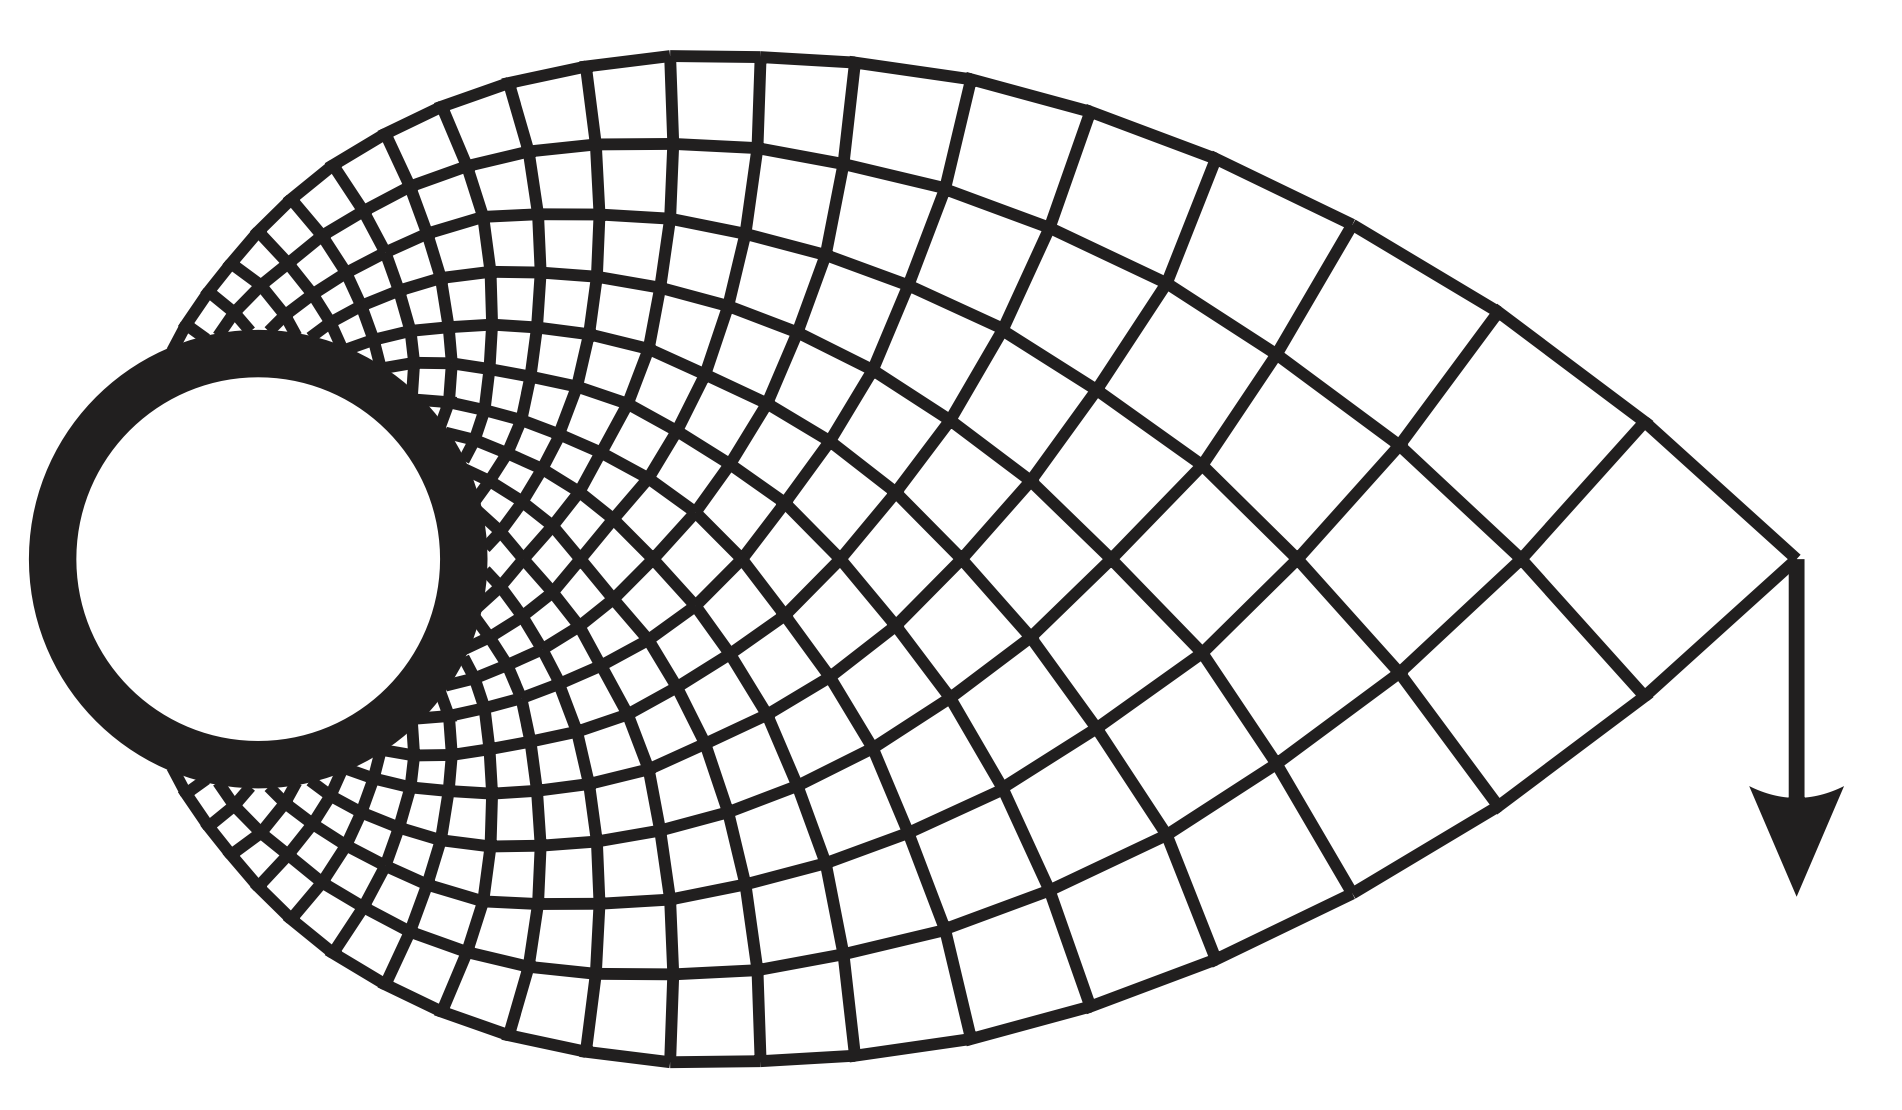
\includegraphics[width=0.5\textwidth]{figures/michell.png}
    \end{center}
    
\end{example}

The problem in Equation \eqref{eq:size_optimization} is convex, but it is not separable and explicit, because we cannot find an explicit expression for $\mathbf{a}^*(\mu)$ at the stationary point of the Lagrangian. Therefore we linearize the problem using MMA in $1/(a_j-L_j^k)$. The linearization of the objective function becomes
\begin{align}
    \tilde{C}(\mathbf{a}) &= C(\mathbf{a}^k) + \sum_j \frac{\partial C}{\partial a_j}(\mathbf{a}^k) (a^k_j-L^k_j) - \sum_j \frac{\partial C}{\partial a_j}(\mathbf{a}^k) \frac{(a^k_j-L^k_j)^2}{a_j-L^k_j}\\
    &=C(\mathbf{a}^k) 
    - \sum_j 2w_j (\mathbf{a}^k) (a^k_j-L^k_j)
    + \sum_j 2w_j (\mathbf{a}^k)
    \frac{(a^k_j-L^k_j)^2}{a_j-L^k_j}.
\end{align}
Note that this is a linearization using lower asymptotes only, because 
\begin{equation}
    \frac{\partial C }{\partial a_j}(\mathbf{a}^k)  = - 2 w_j (\mathbf{a}^k) < 0 \quad \forall \mathbf{a}^k
\end{equation} 
and thus all terms in Equations \eqref{eq:mma_start} and \eqref{eq:mma_end} involving $p_j^k$ vanish.
The approximated optimization problem becomes 
\begin{equation}
    \begin{aligned}
        \min_{\mathbf{a}} \quad & \tilde{C} (\mathbf{a})\\
        \textrm{s.t.} \quad & \mathbf{a} \cdot \mathbf{l} - V_0 \le 0  \\
                            & \tilde{\mathbf{a}}^{l,k} \le \mathbf{a} \le \mathbf{a}^u\\
    \end{aligned}
\end{equation}
with lower move limits $\tilde{\mathbf{a}}^{l,k} = \max(\mathbf{a}^l,  0.9 \mathbf{L}^k + 0.1 \mathbf{a}^k)$ preventing division by zero. The constraint is already linear and thus we do not approximate it.

The Lagrangian of the approximated problem is
\begin{equation}
    \mathcal{L}(\mathbf{a}, \mu) = \tilde{C}(\mathbf{a}) + \mu \left( \mathbf{a} \cdot \mathbf{l} - V_0 \right)
\end{equation}
is separable with 
\begin{equation}
    \begin{split}
        \mathcal{L}(\mathbf{a}, \mu) &= \underbrace{C(\mathbf{a}^k) - \sum_j 2w_j (\mathbf{a}^k) (a^k_j-L^k_j) - \mu V_0}_{\mathcal{L}^0} \\
        &+ \sum_j \underbrace{\left(2 w_j (\mathbf{a}^k)
        \frac{(a^k_j-L^k_j)^2}{a_j-L^k_j} + \mu a_j l_j \right)}_{\mathcal{L}_j (a_j)}.
    \end{split}
\end{equation}
We want to find an explicit expression for $\mathbf{a}^*(\mu)$. Therefore we compute the stationary point of the Lagrangian
\begin{equation}
    \frac{\partial \mathcal{L}_j}{\partial a_j} = -2 w_j (\mathbf{a}^k)
    \frac{(a^k_j-L^k_j)^2}{(\hat{a}_j-L^k_j)^2} + \mu l_j = 0
\end{equation}
and rearrange the equation to find 
\begin{equation}
    \hat{a}_j(\mu) = L_j^k + \sqrt{\frac{2 w_j (\mathbf{a}^k)
    (L^k_j-a^k_j)^2}{\mu l_j}}. 
\end{equation}
We simply clip this result with box constraints to obtain the explicit relation 
\begin{equation}
    \mathbf{a}^* (\mu) = \max\left(\tilde{\mathbf{a}}^{l,k}, \min \left(\hat{\mathbf{a}}(\mu), \mathbf{a}_u \right)\right). 
\end{equation}
Finally we can plug this result in the Lagrangian to get the dual function
\begin{equation}
    \underline{\mathcal{L}}(\mu) = \mathcal{L}(\mathbf{a}^* (\mu), \mu)
\end{equation}
and solve 
\begin{equation}
    \max_{\mu} \underline{\mathcal{L}}(\mu)
\end{equation}
for $\mu^*>0$. This solution procedure is simple - the dual Lagrangian depends only on one variable and the problem is concave. We can use a gradient decent method to solve it quickly and utilize this analytical expression for the gradient 
\begin{equation}
    \frac{\partial \underline{\mathcal{L}}}{\partial \mu}(\mu) =  \mathbf{a}^* (\mu) \cdot \mathbf{l} - V_0.
\end{equation}


\begin{example}{Three bar truss optimization}{trussoptimization example}
    Consider the truss from the previous example. Instead of just computing the displacements, we are now interested in finding the optimal cross sectional areas given a volume constraint.

    We formulate the following algorithm to solve that problem: 
    \begin{enumerate}
        \item Define the truss with all nodes $\mathcal{N}$, elements $\mathcal{E}$, material property $E$, volume constraint $V_0$, design limits $\mathbf{a}^l, \mathbf{a}^u$ and the initial design choice $\mathbf{a}^0$.
        \item Compute the displacements $\mathbf{u}^k = \mathbf{u}(\mathbf{a}^k)$ by solving the truss system for the current design $\mathbf{a}^k$.
        \item Compute the lower asymptotes as $\mathbf{L}^k =\mathbf{a}^k - s (\mathbf{a}^u - \mathbf{a}^l)$ with $s \in (0,1)$ during the first two iterations and according to 
        \begin{equation}
            L^k_j = 
            \begin{cases}
                a^k_j - s  (a^{k-1}_j-L^{k-1}_j) & (a_j^k-a_j^{k-1})(a_j^{k-1}-a_j^{k-2}) < 0\\
                a^k_j - \frac{1}{\sqrt{s}}  (a^{k-1}_j-L^{k-1}_j) & \text{else}
            \end{cases}
        \end{equation}
        in the following iterations.
        \item Compute the lower move limit as 
        \begin{equation}
            \tilde{\mathbf{a}}^{l,k} = \max(\mathbf{a}^l,  0.9 \mathbf{L}^k + 0.1 \mathbf{a}^k)
        \end{equation}
        \item Compute the gradient of the objective function (strain energies per area) for all elements using the previously computed displacements
        \begin{equation}
            w^k_j = \frac{1}{2}\mathbf{u}^k_j  \cdot \mathbf{k}^0_j \cdot \mathbf{u}^k_j
        \end{equation}
        \item Evaluate the analytical solution for
            \begin{align}
                \hat{a}_j(\mu) &= L_j^k + \sqrt{\frac{2 w^k_j
                (L^k_j-a^k_j)^2}{\mu l_j}} \\
                \mathbf{a}^* (\mu) &= \max\left(\tilde{\mathbf{a}}^{l,k}, \min \left(\hat{\mathbf{a}}(\mu), \mathbf{a}_u \right)\right)
            \end{align}
            to define the dual function 
            \begin{equation}
                \underline{\mathcal{L}}(\mu) = \mathcal{L}(\mathbf{a}^* (\mu), \mu)
            \end{equation}
        \item Perform a line search to find the root $\mu^*>0$ in 
        \begin{equation}
            \frac{\partial \underline{\mathcal{L}}}{\partial \mu}(\mu) = \mathbf{l} \cdot \mathbf{a}^* (\mu) - V_0 = 0
        \end{equation}
        with Newton's method or bisection method. 
        \item Repeat with steps 2-7 until convergence or a maximum number of iterations is reached.
    \end{enumerate}

    The following figure plots the three design variables $a_1, a_2, a_3$ for the three bar truss with $\mathbf{a}^0=(0.5,0.2,0.3)^\top$, $\mathbf{a}^l=(0.1,0.1,0.1)^\top$, $\mathbf{a}^u=(1.0,1.0,1.0)^\top$ and $V_0=0.5$. After a couple of iterations, the solution converges towards the analytical solution plotted in gray.

    \begin{minipage}{.5\textwidth}
        \centering
        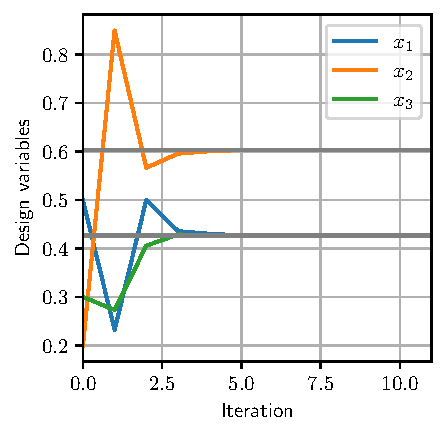
\includegraphics[width=0.9\linewidth]{figures/three_bar_truss_variables.pdf}
    \end{minipage}%
    \begin{minipage}{.5\textwidth}
        \centering
        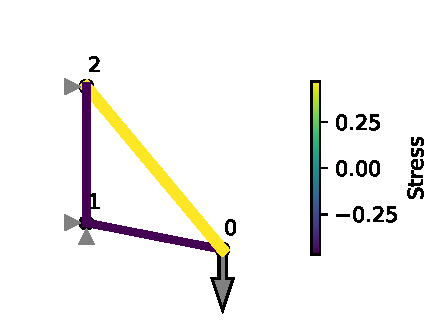
\includegraphics[width=0.9\linewidth]{figures/three_bar_truss_optimized.pdf}
    \end{minipage}
       
\end{example}

\begin{example}{Truss optimization}{trussoptimizationexample}
    The following figure plots the deformed configuration of a size optimization result for the truss shown in Figure \ref{fig:truss_example}. Line thicknesses correspond to the design variables and colors indicate stresses. Note that this is not a fully stressed design (the stress magnitudes are not all identical), because some design variables reach their upper limit. Essentially, the outcome is close to a topology optimization, because it indicates elimination of some elements. However, a complete elimination is not possible as this would result in a singular stiffness matrix, i.e. the displacement of node 9 would be undetermined. 

    \begin{center}
        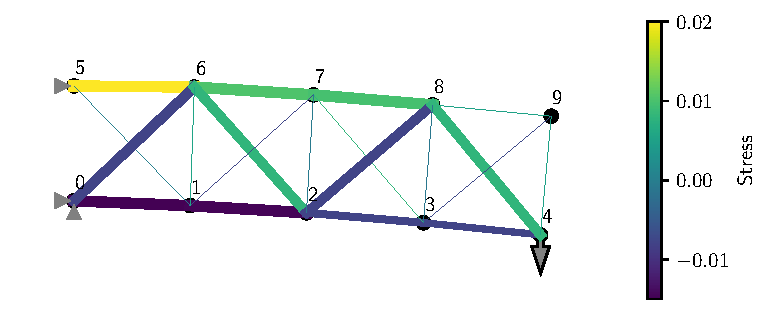
\includegraphics[width=0.9\textwidth]{figures/truss_sample_optimized.pdf} 
    \end{center}
\end{example}

\begin{example}{Large truss optimization}{largetrussoptimizationexample} 
    We could solve very simple truss optimization problems, like the three bar problem above, analytically. Hence, the applied method with MMA seems a bit overkill. 
    However, we cannot solve the optimization problem for large structures like the truss below analytically. 

    \begin{center}
        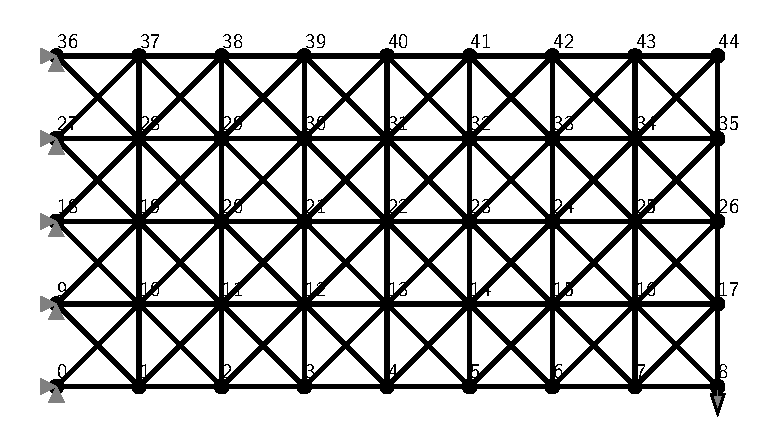
\includegraphics[width=0.75\textwidth]{figures/large_truss.pdf} 
    \end{center}

    In this case, the truss was optimized with large enough upper limits for the cross sections such that the resulting optimized structure is fully stressed. We may interpret the resulting structure effectively as a four bar truss with optimal cross sections. Note that we did not consider instability problems like buckling, so before building a truss structure like this we should check it for buckling instabilities.

    \begin{center}
        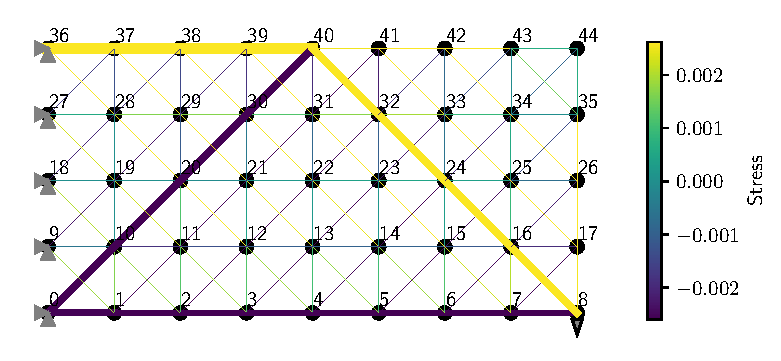
\includegraphics[width=0.9\textwidth]{figures/large_truss_optimized.pdf} 
    \end{center}
\end{example}

\section{Topology optimization}
\label{sec:truss_topology}
In topology optimization of trusses, we want to identify those bars which should stay in our design and those trusses which may be removed. As seen in the last examples of the previous chapter, this is closely related to size optimization - the difference is that we seek a binary design (bar or no bar) instead of continuous cross section variables. Hence, we change the box constraint to a discrete constraint with a bar being either at maximum cross sectional area or minimum cross sectional area, but nothing in between.

The topology optimization problem of minimizing compliance for a given volume constraint has similar structure as the size optimization problem. The only change is that $\mathbf{a}$ is now either the maximum or minimum cross section. Thus, we formally have 
\begin{equation}
    \begin{aligned}
        \min_{\mathbf{a}} \quad & C(\mathbf{a}) = \mathbf{f} \cdot \mathbf{u}(\mathbf{a})\\
        \textrm{s.t.} \quad & \mathbf{a} \cdot \mathbf{l} - V_0 \le 0  \\
                            & a_j \in \{a_j^l, a_j^u\}\\
    \end{aligned}
\end{equation}

Unfortunately, the binary problem is notoriously hard to solve, because we cannot compute gradients on the solution and testing all solutions is computationally inaccessible. Hence we try to formulate a continuous relation between stiffness and a normalized variable $\rho_j = a_j/a_j^u$ that still results in a binary result. One such formulation is called \emph{Solid Isotropic Material with Penalization} (SIMP) and we denote it here as 
\begin{equation}
    E(\rho_j)= \rho_j^p E
\end{equation}
with a penalization parameter $p \ge 1$. 
The effect of penalization is shown in Figure \ref{fig:simp_truss} for typical values of $p$. We may observe for $p>1$ that the stiffness per invested material is unattractive for intermediate density values. For example, choosing $\rho_j^u=0.5$ with $p=2$ adds half an element volume to the total volume, but contributes only a quarter of the stiffness compared to a fully filled element. An optimization that tries to minimize compliance for a given volume will therefore rather favor elements that provide the full stiffness benefit or add only a minimal contribution to the total volume.

\begin{figure}[!htpb]
    \centering
    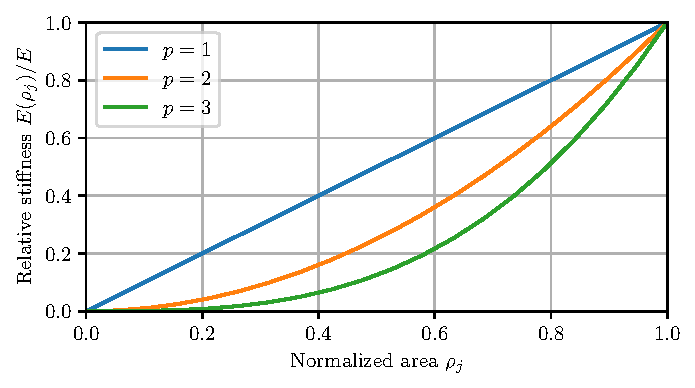
\includegraphics[width=0.9\textwidth]{figures/simp_truss.pdf}
    \caption{Penalization factors in SIMP.}
    \label{fig:simp_truss}
\end{figure}

Hence, the topology optimization problem with SIMP becomes  
\begin{equation}
    \begin{aligned}
        \min_{\pmb{\rho}} \quad & C(\pmb{\rho}) = \mathbf{f} \cdot \mathbf{u}(\pmb{\rho})\\
        \textrm{s.t.} \quad & \pmb{\rho} \cdot \mathbf{V} - V_0 \le 0  \\
                            & \rho_j \in (0, 1]
    \end{aligned}
\end{equation}
where $V_j=a_j l_j$ describes the element volumes and $\rho_j >0$ prevents singularities. After introducing SIMP, the overall problem structure is (besides the different variable names) equivalent to the size optimization problem. The only change in comparison to size optimization  is the computation of the sensitivity
\begin{align}
    \frac{\partial C (\pmb{\rho})}{\partial \rho_j} 
    &= - \mathbf{u}_j (\pmb{\rho}) \cdot \frac{\partial \mathbf{k}_j(\rho_j)}{\partial \rho_j} \cdot \mathbf{u}_j (\pmb{\rho})  \\
    &= - p \rho_j^{p-1} \mathbf{u}_j (\pmb{\rho}) \cdot \mathbf{k}^0_j \cdot \mathbf{u}_j (\pmb{\rho})  \\
    &= - 2 p \rho_j^{p-1} w_j (\pmb{\rho}),
\end{align}
which now accounts for the penalty factor. Note that for $p=1$, this is identical to Equation \eqref{eq:compliance_sensitivity}. 
The entire remaining approximation procedure and solution procedure is identical to the size optimization discussed in the previous section.

\section{Shape optimization}
So far, we have performed size optimization of trusses by adjusting the cross sectional areas and we have performed topology optimization of trusses by allowing bars to disappear. However, the node positions remained fixed in all these cases. 
In this section, we want to optimize the position of nodes $\mathbf{x}$ for a fixed topology $\mathcal{E}$ and fixed cross sectional areas $\mathbf{a}$.

The truss shape optimization for minimum compliance with a volume constraint has a structure similar to the previous problems. However, the design variable changes to the nodal positions $\mathbf{x}$ or a subset of those nodal positions (if not all nodes are allowed to change position). While the cross sectional areas of the constraint are fixed, the element lengths are a function of design variables now. The full shape optimization problem may be denoted as follows:
\begin{equation}
    \begin{aligned}
        \min_{\mathbf{x}} \quad & C(\mathbf{x}) = \mathbf{f} \cdot \mathbf{u}(\mathbf{x})\\
        \textrm{s.t.} \quad & g(\mathbf{x}) = \mathbf{a} \cdot \mathbf{l}(\mathbf{x}) - V_0 \le 0  \\
                            & \mathbf{x} \in \mathcal{X}\\
    \end{aligned}
    \label{eq:shape_optimization}
\end{equation}

% \subsection{Analysis of problem}
% We formulate the Lagrangian of the shape optimization problem as 
% \begin{equation}
%     \mathcal{L}(\mathbf{x}, \mu) = C(\mathbf{x}) + \mu g(\mathbf{x})
% \end{equation}
% and compute gradients to find KKT points. The gradient of the Lagrangian w.r.t $\mathbf{x}$ is  
% \begin{equation}
%     \frac{\partial \mathcal{L} (\mathbf{x}, \mu)}{\partial x_i} 
%     = \frac{\partial C (\mathbf{x})}{\partial x_i} + \mu \mathbf{a} \cdot \frac{\partial \mathbf{l}(\mathbf{x})}{\partial x_i}.
%     \label{eq:lagrange_truss_shape_problem}
% \end{equation}
% # def dkdx(self, j):
% #     element = self.elements[j]
% #     n1 = element[0]
% #     n2 = element[1]
% #     dx = self.nodes[n1][0] - self.nodes[n2][0]
% #     dy = self.nodes[n1][1] - self.nodes[n2][1]
% #     l0 = torch.sqrt(dx**2 + dy**2)
% #     c = dx / l0
% #     s = dy / l0
% #     m = torch.tensor(
% #         [
% #             [c**2, s * c, -(c**2), -s * c],
% #             [s * c, s**2, -s * c, -(s**2)],
% #             [-(c**2), -s * c, (c**2), s * c],
% #             [-s * c, -(s**2), s * c, s**2],
% #         ]
% #     )
% #     dmdphi = torch.tensor(
% #         [
% #             [-2 * s * c, c**2 - s**2, 2 * s * c, s**2 - c**2],
% #             [c**2 - s**2, 2 * s * c, s**2 - c**2, -2 * s * c],
% #             [2 * s * c, s**2 - c**2, -2 * s * c, c**2 - s**2],
% #             [s**2 - c**2, -2 * s * c, c**2 - s**2, 2 * s * c],
% #         ]
% #     )
% #     dkdx1 = (
% #         -self.areas[j] * self.E * dx / l0**3 * m
% #         - self.areas[j] * self.E / l0 * dmdphi * dy
% #     )
% #     dkdx2 = (
% #         -self.areas[j] * self.E * dy / l0**3 * m
% #         + self.areas[j] * self.E / l0 * dmdphi * dx
% #     )
% #     dkdx3 = (
% #         self.areas[j] * self.E * dx / l0**3 * m
% #         + self.areas[j] * self.E / l0 * dmdphi * dy
% #     )
% #     dkdx4 = (
% #         self.areas[j] * self.E * dy / l0**3 * m
% #         - self.areas[j] * self.E / l0 * dmdphi * dx
% #     )
% #     return [dkdx1, dkdx2, dkdx3, dkdx4]

Both, the target function $C(\mathbf{x})$ and the constraint $g(\mathbf{x})$, are in general non-linear non-separable functions. Hence, we apply MMA to both functions to get sequential convex explicitly separable approximations.
We can denote the Lagrangian of the approximated functions as 
\begin{align}
    \mathcal{L}(\mathbf{x}, \mu) &= \tilde{C}(\mathbf{x}) + \mu \tilde{g}(\mathbf{x})
    \label{eq:shape_lagrangian}
\end{align}
which is a separable function and we can use it to solve the problem with the dual method. We need to distinguish cases for each separable term $\mathcal{L}_i(x_i, \mu)$ as the MMA approximations are different depending on the signs of $\frac{\partial C}{\partial x_i} (\mathbf{x}^k)$ and $\frac{\partial g}{\partial x_i} (\mathbf{x}^k)$. Hence, we distinguish four cases for the gradient computation:
\begin{equation}
    \frac{\partial \mathcal{L}_i (\mathbf{x}, \mu)}{\partial x_i} = 
    \begin{cases}
        \left(\frac{U_i^k-x_i^k}{U_i^k-x_i}\right)^2 \left(\frac{\partial C}{\partial x_i} + \mu \frac{\partial g}{\partial x_i} \right) 
            &\textrm{if} \quad \frac{\partial C}{\partial x_i} > 0, \frac{\partial g}{\partial x_i} > 0 \\
        \left(\frac{U_i^k-x_i^k}{U_i^k-x_i}\right)^2 \frac{\partial C}{\partial x_i}  + \mu \left(\frac{x_i^k-L_i^k}{x_i-L_i^k}\right)^2 \frac{\partial g}{\partial x_i} 
            &\textrm{if} \quad \frac{\partial C}{\partial x_i}  > 0, \frac{\partial g}{\partial x_i} <0\\
        \left(\frac{x_i^k-L_i^k}{x_i-L_i^k}\right)^2 \frac{\partial C}{\partial x_i}  + \mu \left(\frac{U_i^k-x_i^k}{U_i^k-x_i}\right)^2\frac{\partial g}{\partial x_i} 
            &\textrm{if} \quad \frac{\partial C}{\partial x_i} < 0, \frac{\partial g}{\partial x_i}  > 0\\
        \left(\frac{x_i^k-L_i^k}{x_i-L_i^k}\right)^2 \left(\frac{\partial C}{\partial x_i}  + \mu \frac{\partial g}{\partial x_i} \right) 
            &\textrm{if} \quad \frac{\partial C}{\partial x_i}< 0, \frac{\partial g}{\partial x_i}< 0
    \end{cases}
\end{equation}
where all gradients are evaluated at $\mathbf{x}^k$.
To find the potential minimum $\hat{x}_i(\mu)$, we investigate for each case individually, under which conditions it vanishes. For the first case, the second term is always positive considering the KKT condition $\mu>0$. Therefore we find that in this case $x\rightarrow -\infty$ would be a minimum. Using the box constraint this yields $\hat{x}_i(\mu) = x^l_i$. Analogously, the last case yields $\hat{x}_i(\mu) = x^u_i$. The other cases are solved simply by re-arranging the equations and finally we get 
\begin{equation}
    \hat{x}_i (\mu) = 
    \begin{cases}
        x^l_i 
            &\textrm{if} \quad \frac{\partial C}{\partial x_i} > 0, \frac{\partial g}{\partial x_i} > 0 \\
        \frac{U_i^k\omega + L_i^k}{1+\omega} \quad \text{with} \quad \omega = \sqrt{-\mu\frac{(x_i^k-L_i^k)^2\frac{\partial g}{\partial x_i}}{(U_i^k-x_i^k)^2\frac{\partial C}{\partial x_i}}}
            &\textrm{if} \quad \frac{\partial C}{\partial x_i}  > 0, \frac{\partial g}{\partial x_i} <0\\
        \frac{U_i^k-L_i^k\omega}{1+\omega} \quad \text{with} \quad \omega = \sqrt{-\mu\frac{(U_i^k-x_i^k)^2\frac{\partial g}{\partial x_i}}{(x_i^k-L_i^k)^2\frac{\partial C}{\partial x_i}}} 
            &\textrm{if} \quad \frac{\partial C}{\partial x_i} < 0, \frac{\partial g}{\partial x_i}  > 0\\
        x^u_i 
            &\textrm{if} \quad \frac{\partial C}{\partial x_i}< 0, \frac{\partial g}{\partial x_i} < 0.
    \end{cases}
\end{equation}
With move limits $\tilde{\mathbf{x}}^{l,k}$ and $\tilde{\mathbf{x}}^{u,k}$ according to Equation \eqref{eq:mma_move_limits}, we can find the box-constrained minimum of the approximated Lagrangian w.r.t to $\mathbf{x}$ as
\begin{equation}
    \mathbf{x}^*(\mu) = \max\left(\tilde{\mathbf{x}}^{l,k}, \min \left(\hat{\mathbf{x}}(\mu), \tilde{\mathbf{x}}^{u,k} \right)\right).
\end{equation}
Finally we can plug this result in the Lagrangian to get the dual fucntion 
\begin{equation}
    \underline{\mathcal{L}}(\mu) = \mathcal{L}(\mathbf{x}^* (\mu), \mu)
\end{equation}
and solve 
\begin{equation}
    \max_{\mu} \underline{\mathcal{L}}(\mu)
    \label{eq:shape_dual_solution}
\end{equation}
for $\mu^*>0$. 

\begin{example}{Three bar truss shape optimization}{trussshapeoptimizationexample}
    Consider the truss from the previous chapter. Instead of computing optimal cross sectional areas, we now want to optimize its shape. To do so, we allow Node 0 and Node 2 to move a certain amount up or down. These two design variables are 
    \begin{equation}
        \mathbf{x} = 
        \begin{pmatrix}
            x_0^2 \\ x_2^0
        \end{pmatrix}
    \end{equation}
    and they are constrained by 
    \begin{equation}
        \mathbf{x}^l = 
        \begin{pmatrix}
             -0.5\\ 0.5
        \end{pmatrix} 
        \quad 
        \text{and}
        \quad
        \mathbf{x}^u = 
        \begin{pmatrix}
             0.5\\ 1.5
        \end{pmatrix} 
    \end{equation}
    The range of motion is illustrated in the following Figure:
    \begin{center}
        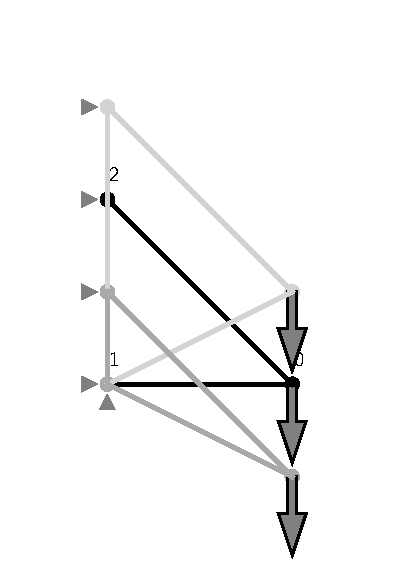
\includegraphics[width=0.4\linewidth]{figures/three_bar_truss_shapes.pdf}
    \end{center}

    We want to solve for the optimal shape $\mathbf{x}^*$ that minimizes the compliance of the structure without exceeding the initial volume of the truss. The original optimization problem and the MMA approximation are illustrated in the following two plots on the left and right, respectively.

    \begin{minipage}{.5\textwidth}
        \centering
        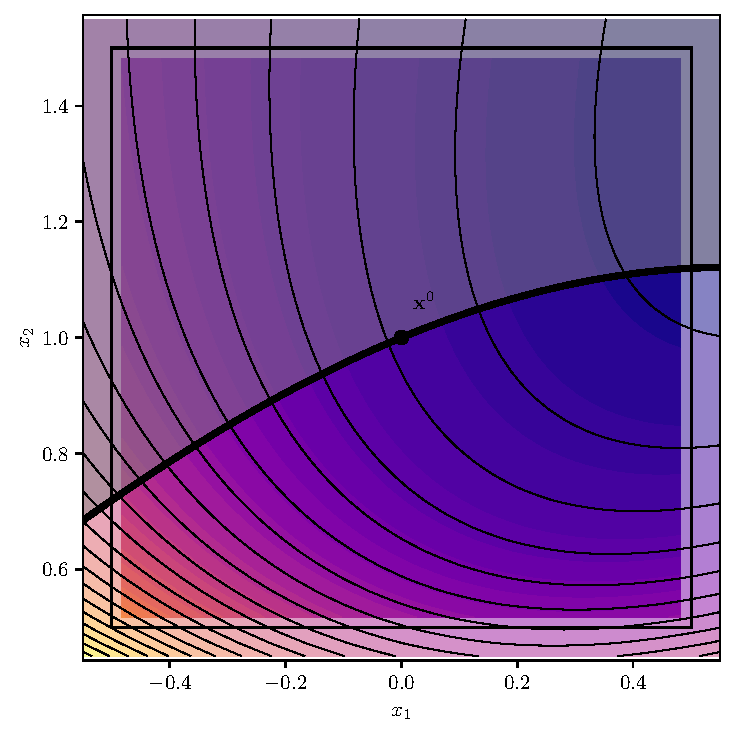
\includegraphics[width=0.9\linewidth]{figures/three_bar_truss_shape_original.pdf}
    \end{minipage}%
    \begin{minipage}{.5\textwidth}
        \centering
        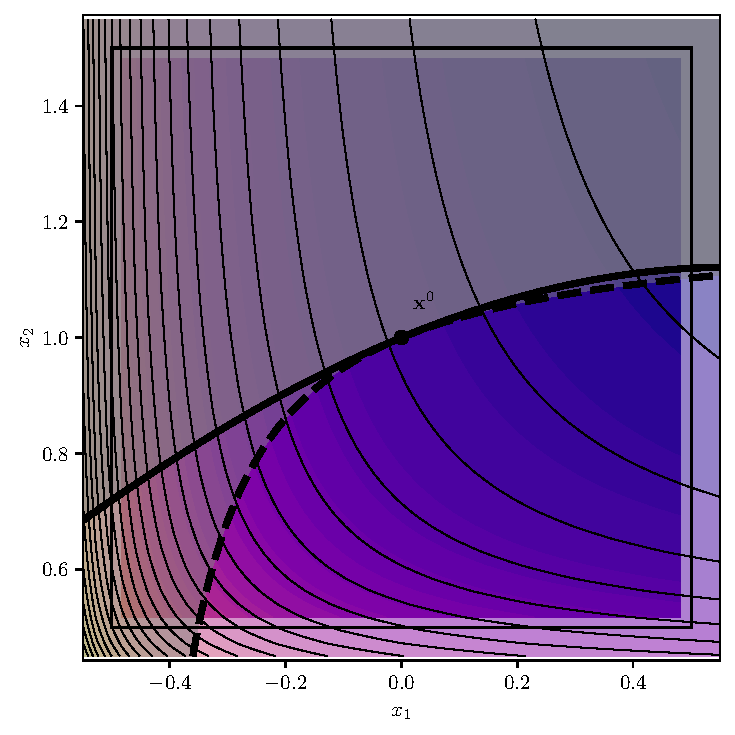
\includegraphics[width=0.9\linewidth]{figures/three_bar_truss_shape_mma.pdf}
    \end{minipage}

    We formulate the following algorithm to solve the approximated problem: 
    \begin{enumerate}
        \item Define the truss with all nodes $\mathcal{N}$, elements $\mathcal{E}$, material property $E$, volume constraint $V_0$, design limits $\mathbf{x}^l, \mathbf{x}^u$ and the initial design choice $\mathbf{x}^0$.
        \item Compute the displacements $\mathbf{u}^k$ by solving the truss system for the current design $\mathbf{x}^k$.
        \item Compute the asymptotes as $\mathbf{L}^k =\mathbf{x}^k - s (\mathbf{x}^u - \mathbf{x}^l)$ and $\mathbf{U}^k =\mathbf{x}^k + s (\mathbf{x}^u - \mathbf{x}^l)$ with $s \in (0,1)$ during the first two iterations. In the following iterations, compute the lower asymptotes according to 
        \begin{equation}
            L^k_i = 
            \begin{cases}
                x^k_i - s  (x^{k-1}_i-L^{k-1}_i) & (x_i^k-x_i^{k-1})(x_i^{k-1}-x_i^{k-2}) < 0\\
                x^k_i - \frac{1}{\sqrt{s}}  (x^{k-1}_i-L^{k-1}_i) & \text{else}
            \end{cases}
        \end{equation}
        and the upper asymptotes according to 
        \begin{equation}
            U^k_i = 
            \begin{cases}
                x^k_i - s  (U^{k-1}_i-x^{k-1}_i) & (x_i^k-x_i^{k-1})(x_i^{k-1}-x_i^{k-2}) < 0\\
                x^k_i - \frac{1}{\sqrt{s}}  (U^{k-1}_i-x^{k-1}_i) & \text{else}
            \end{cases}
        \end{equation}

        \item Compute the move limits as 
        \begin{align}
            \tilde{\mathbf{x}}^{l,k} &= \max(\mathbf{x}^l,  0.9 \mathbf{L}^k + 0.1 \mathbf{x}^k) \\
            \tilde{\mathbf{x}}^{u,k} &= \min(\mathbf{x}^u,  0.9 \mathbf{U}^k + 0.1 \mathbf{x}^k)
        \end{align}

        \item Evaluate the gradients of the objective function $\frac{\partial C}{\partial x_i}$ and the constraint $\frac{\partial g}{\partial x_i}$ at $\mathbf{x}^k$ using automatic differentiation. 

        \item Evaluate the analytical solution
            \begin{align}
                \hat{x}_i(\mu) &= 
                \begin{cases}
                    x^l_i 
                        &\textrm{if} \quad \frac{\partial C}{\partial x_i} > 0, \frac{\partial g}{\partial x_i} > 0 \\
                    \frac{U_i^k\omega + L_i^k}{1+\omega}, \quad \omega = \sqrt{-\mu\frac{(x_i^k-L_i^k)^2\frac{\partial g}{\partial x_i}}{(U_i^k-x_i^k)^2\frac{\partial C}{\partial x_i}}}
                        &\textrm{if} \quad \frac{\partial C}{\partial x_i}  > 0, \frac{\partial g}{\partial x_i} <0\\
                    \frac{U_i^k-L_i^k\omega}{1+\omega}, \quad \omega = \sqrt{-\mu\frac{(U_i^k-x_i^k)^2\frac{\partial g}{\partial x_i}}{(x_i^k-L_i^k)^2\frac{\partial C}{\partial x_i}}} 
                        &\textrm{if} \quad \frac{\partial C}{\partial x_i} < 0, \frac{\partial g}{\partial x_i}  > 0\\
                    x^u_i 
                        &\textrm{if} \quad \frac{\partial C}{\partial x_i}< 0, \frac{\partial g}{\partial x_i} < 0.
                \end{cases} \\
                \mathbf{x}^* (\mu) &= \max\left(\tilde{\mathbf{x}}^{l,k}, \min \left(\hat{\mathbf{x}}(\mu), \tilde{\mathbf{x}}^{u,k} \right)\right)
            \end{align}
        \item Perform a line search to find the maximum in 
            \begin{equation}
                \max_{\mu>0} \underline{\mathcal{L}}(\mu)
            \end{equation}
            with a gradient decent method. Once again, we may use automatic differentiation to compute the gradient for the optimization.
        \item Repeat with steps 2-7 until convergence or a maximum number of iterations is reached.
    \end{enumerate}
    
    The following figures plot the optimization path and the optimal truss shape for the final solution $\mathbf{x}^* = (0.5, 1.12)^\top$ (black) as well as the initial configuration $\mathbf{x}^0 = (0.0, 1.0)^\top$ (gray).

    \begin{minipage}{.5\textwidth}
        \centering
        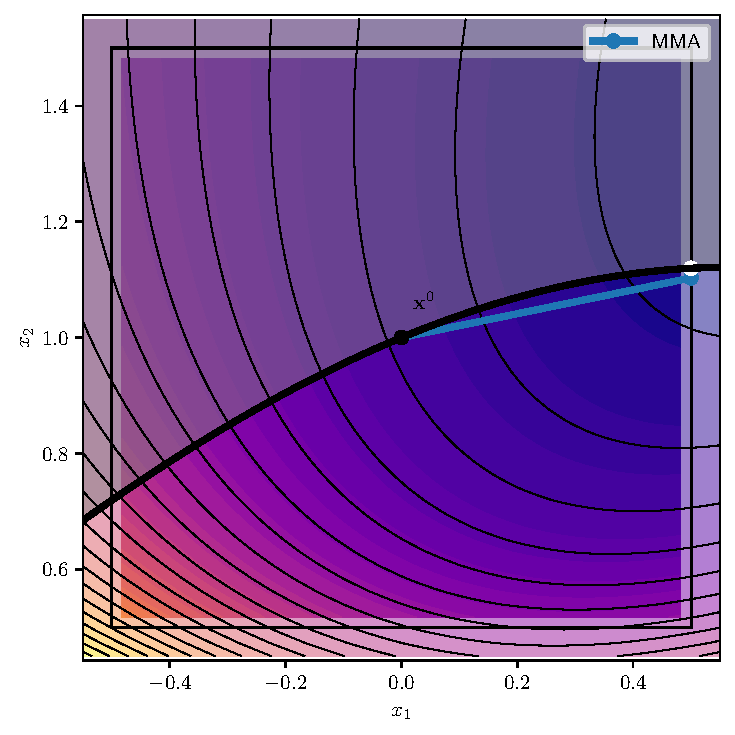
\includegraphics[width=0.9\linewidth]{figures/three_bar_truss_shape_optimization.pdf}
    \end{minipage}%
    \begin{minipage}{.5\textwidth}
        \centering
        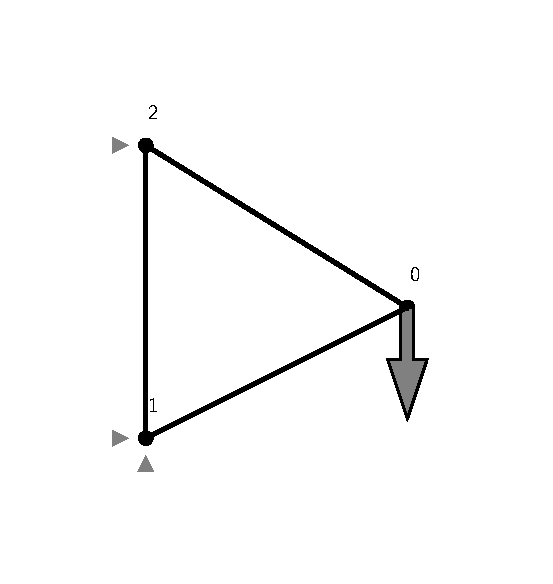
\includegraphics[width=0.9\linewidth]{figures/three_bar_truss_shape_optimized.pdf}
    \end{minipage}
       
\end{example}

\bibliographystyle{unsrtnat}
\bibliography{literature} 






\chapter{Finite element analysis in a nutshell}
In the previous chapters we learned to optimize discrete truss structures. However, most structures are not discrete by nature. They are continua and need to be transferred to a discrete representation for structural optimization. The most common method for this is the \emph{Finite Element Method} (FEM) and we quickly summarize this method in this chapter for further use in structural optimization. If you are interested in more details, you may refer to the excellent book by Fish and Belytschko \cite{Fish2007}.

\begin{objectives}{}{objectives_fem}
After studying this chapter and finishing the exercise, you should be able to 
\begin{itemize}[label=$\dots$]
    \item explain why we need finite elements in the first place 
    \item cite the linear elastic problem for an isotropic material
    \item formulate the weak form of the linear elastic problem and explain advantages of that formulation
    \item describe the concept of discretization by finite elements 
    \item formulate the shape functions and derivatives for a 2D quadrilateral linear element 
    \item transform the weak form into a linear system of equations using shape functions and numerical integration
    \item assemble the global FEM system and draw analogies to truss systems
\end{itemize}
\end{objectives}

\section{The linear elastic problem}
The fundamental equation to solve in static structural problems is the balance of linear momentum
\begin{equation}
    \nabla \cdot \mathbf{S}(\mathbf{x}) + \mathbf{b}(\mathbf{x})= \mathbf{0} 
    \quad 
    \mathbf{x} \in \Omega
    \label{eq:linear_momentum_balance}
\end{equation}
with the symmetric stress tensor $\mathbf{S}=\mathbf{S}^\top \in \mathcal{R}^{d \times d}$ and a prescribed body force field $\mathbf{b} \in \mathcal{R}^d$ describing a force per volume. The term \emph{static} means that we do not consider any time derivatives, i.e. we are searching for a stationary solution.  The domain $\Omega$ describes for example all points of a structural component and we use $\partial \Omega$ to denote the boundary of that domain. This equilibrium basically states that the divergence of stresses (inner forces) must balance the body force field in all points of a domain $\Omega$ to remain stationary. 

The stress tensor is related to the engineering strain tensor 
\begin{equation}
    \mathbf{E}(\mathbf{u}) = \frac{1}{2} \left(\nabla \mathbf{u} + \left(\nabla \mathbf{u}\right)^\top \right)
    \label{eq:strain}
\end{equation} 
via a linear elastic material model 
\begin{equation}
    \mathbf{S}(\mathbf{x})  = \mathbb{C}  : \mathbf{E}(\mathbf{u}) 
    \label{eq:linear_elasticity}
\end{equation}
with a stiffness tensor $\mathbb{C}  \in \mathcal{R}^{d \times d \times d \times d}$. Here, it is assumed that $\mathbb{C}$ does not depend on the position $\mathbf{x}$, i.e. the same material is used in the entire structure. In case of an isotropic material, i.e. a material that behaves direction-independent, we can write Equation \eqref{eq:linear_elasticity} as
\begin{equation}
    \mathbf{S}(\mathbf{x}) = \mathbb{C}_\textrm{iso}  : \mathbf{E}(\mathbf{u})  =  2 G \mathbf{E}(\mathbf{u})  + \Lambda \textrm{tr}(\mathbf{E}(\mathbf{u}) ) \mathbf{I},
    \label{eq:isotropic_material}
\end{equation}
with so-called the Lamé constants 
\begin{equation}
    G = \frac{E}{2(1+\nu)} > 0 
    \quad \text{and} \quad 
    \Lambda = \frac{E\nu}{(1+\nu)(1-2\nu)} > 0 .
\end{equation} 
These two constants, respectively the two constants Young's modulus $E$ and Poisson ratio $\nu$ uniquely describe a linear elastic material. 

\begin{figure}[!htpb]
    \centering
    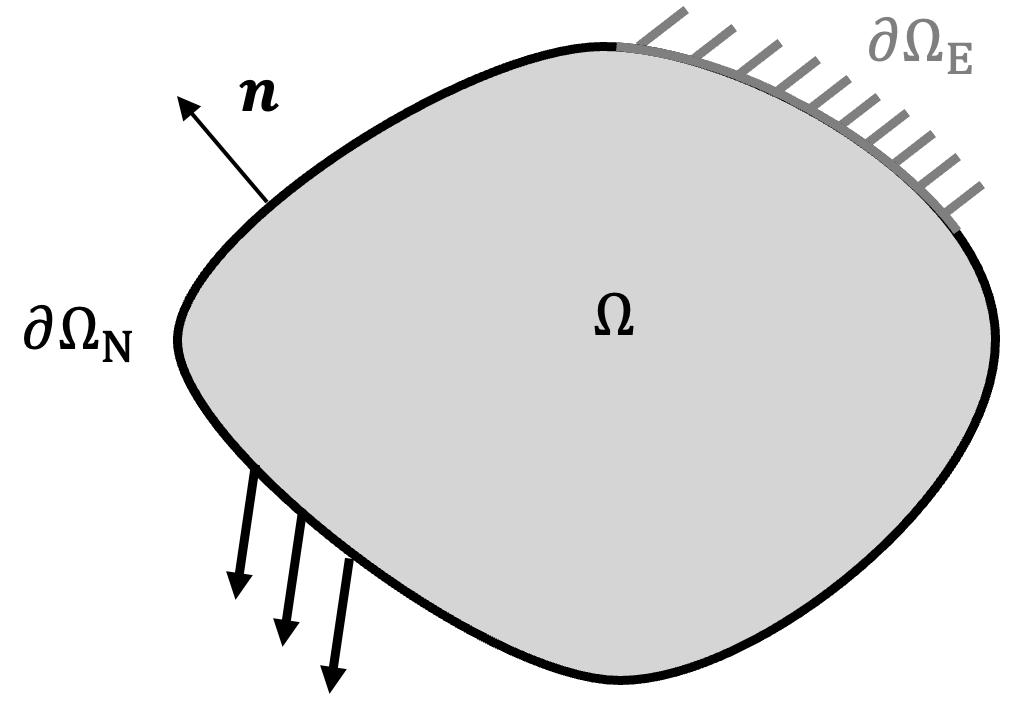
\includegraphics[width=0.5\textwidth]{figures/boundaries.png}
    \caption{The domain $\Omega$ has a boundary $\partial \Omega = \partial \Omega_E \cup \partial \Omega_N, \partial \Omega_E \cap \partial \Omega_N = \emptyset$. We prescribe a displacement $\mathbf{u}_0$ at the essential boundary $\partial \Omega_E$ illustrated with gray lines in the image. The remaining boundary $\partial \Omega_N$ is subjected to a surface traction $\mathbf{t}(\mathbf{x})$. The surface takes the form of a force per boundary unit, e.g. Newton per Meter in a two-dimensional problem with a one-dimensional boundary.}
    \label{fig:boundaries}
\end{figure}

% After substituting the constant isotropic linear elastic material model from Equation \eqref{eq:isotropic_material} in Equation \eqref{eq:linear_momentum_balance} we get Navier's equation
% \begin{equation}
%     (\Lambda + G) \nabla \cdot \left( \nabla \mathbf{u}(\mathbf{x}) 
% \right)
%     + G \nabla^2 \mathbf{u}(\mathbf{x})  + \mathbf{b}(\mathbf{x})  = \mathbf{0}.
%     \label{eq:navier}
% \end{equation}
% In this equation, displacements $\mathbf{u}(\mathbf{x})  \in \mathcal{R}^d$ are the only unknowns. 
% We may write Equation \eqref{eq:navier} more explicitly for the three-dimensional case by expanding it to
% \begin{align}
%     \label{eq:momentum_balance_mat_1}
%     (\Lambda + G) \left( \frac{\partial^2 u_1}{\partial x_1^2} + \frac{\partial^2 u_2}{\partial x_1 \partial x_2} + \frac{\partial^2 u_3}{\partial x_1 \partial x_3}\right)
%     + G \left( \frac{\partial^2 u_1}{\partial x_1^2} + 
%         \frac{\partial^2 u_1}{\partial x_2^2} + \frac{\partial^2 u_1}{\partial x_3^2} 
%     \right) + b_1 &= 0 \\
%     \label{eq:momentum_balance_mat_2}
%     (\Lambda + G) \left( \frac{\partial^2 u_1}{\partial x_1 \partial x_2} + \frac{\partial^2 u_2}{\partial x_2^2} + \frac{\partial^2 u_3}{\partial x_2 \partial x_3}\right)
%     + G \left( \frac{\partial^2 u_2}{\partial x_1^2} + 
%         \frac{\partial^2 u_2}{\partial x_2^2} + \frac{\partial^2 u_2}{\partial x_3^2} 
%     \right) + b_2 &= 0 \\
%     \label{eq:momentum_balance_mat_3}
%     (\Lambda + G) \left( \frac{\partial^2 u_1}{\partial x_1 \partial x_3} + \frac{\partial^2 u_2}{\partial x_2 \partial x_3} + \frac{\partial^2 u_3}{\partial x_3^2}\right)
%     + G \left( \frac{\partial^2 u_2}{\partial x_1^2} + 
%         \frac{\partial^2 u_2}{\partial x_2^2} + \frac{\partial^2 u_2}{\partial x_3^2} 
%     \right) + b_3 &= 0 
% \end{align}
% and observe that we have three partial differential equations for three unknowns $u_1(\mathbf{x}), u_2(\mathbf{x}), u_3(\mathbf{x})$.
With essential boundary conditions on $\partial \Omega_E$ and natural boundary conditions on $\partial \Omega_N$ (see Figure \ref{fig:boundaries}) we can formulate the boundary value problem of linear elasticity as 
\begin{align}
    \nabla \cdot \mathbf{S}(\mathbf{x}) + \mathbf{b}(\mathbf{x}) &= \mathbf{0} 
        &\mathbf{x} \in \Omega \\
    \mathbf{u}(\mathbf{x}) 
    &= \mathbf{u}_0 (\mathbf{x}) 
        &\mathbf{x} \in \partial \Omega_E \\
    \mathbf{S}(\mathbf{x}) \cdot \mathbf{n}(\mathbf{x}) 
    &= \mathbf{t} (\mathbf{x}) 
        &\mathbf{x} \in \partial \Omega_N\\
    \textrm{s.t.} \quad \mathbf{S} &= \mathbb{C} : \mathbf{E}(\mathbf{u})
\end{align}
 which should be solved for displacements $\mathbf{u}(\mathbf{x})$. This is a problem with three partial differential equations for three unknowns $u_1(\mathbf{x}), u_2(\mathbf{x}), u_3(\mathbf{x})$.
Note that this is a second order problem, as we have to compute second derivatives of $\mathbf{u}$ in this problem, as it is differentiated once by $\mathbf{E}(\mathbf{u})$ and then once by $\nabla \cdot \mathbf{S}(\mathbf{x})$.

% \begin{example}{Plane stress}{planestressexample} 
%     We may reduce the elastic problem to two dimensions, if we make an assumption about the third dimension. If we analyze a structure that is very thin in the 3-direction, e.g. a plate or membrane, there are no out-of-plane stress components and we may assume \emph{plane stress}, i.e. $S_{13}=S_{23}=S_{33}=0$ and $\frac{\partial S_{11}}{\partial x_3}=\frac{\partial S_{12} }{\partial x_3}=\frac{\partial S_{22}}{\partial x_3}=0$. 
    
%     Consider a two-dimensional rectangle $\Omega = [0,l]^2$ which is subjected to the following essential boundary conditions
%     \begin{equation}
%         u_1(0, x_2) = 0     \quad
%         u_1(l, x_2) = u_0   \quad
%         u_2(x_1, 0) = 0
%     \end{equation}
%     and the following natural boundary conditions 
%     \begin{equation}
%         S_{12}(x_1, 0) = 0  \quad
%         S_{12}(x_1, l) = 0  \quad
%         S_{22}(x_1, 0) = 0  \quad
%         S_{22}(x_1, l) = 0.
%     \end{equation}

%     Show that 
%     \begin{equation}
%         u_1 (\mathbf{x}) = u_0 \frac{x_1}{l} \quad
%         u_2 (\mathbf{x}) = - u_0 \nu \frac{x_2}{l} \quad
%         u_3 (\mathbf{x}) = - u_0 \nu \frac{x_3}{l}
%     \end{equation}
%     solves the isotropic linear elastic problem.

%     \begin{center}
%         
\includegraphics[width=0.5\textwidth]{figures/rectangle.png}
%     \end{center}
    

%     For plane stress without body forces, the momentum balance reduces to
%     \begin{align}
%         (\Lambda + G) \left( \frac{\partial^2 u_1}{\partial x_1^2} + \frac{\partial^2 u_2}{\partial x_1 \partial x_2} \right)
%         + G \left( \frac{\partial^2 u_1}{\partial x_1^2} + 
%             \frac{\partial^2 u_1}{\partial x_2^2} 
%         \right) &= 0 \\
%         (\Lambda + G) \left( \frac{\partial^2 u_1}{\partial x_1 \partial x_2} + \frac{\partial^2 u_2}{\partial x_2^2} \right)
%         + G \left( \frac{\partial^2 u_2}{\partial x_1^2} + 
%             \frac{\partial^2 u_2}{\partial x_2^2}
%         \right) &= 0. 
%     \end{align}
%     We can easily see that all partial derivatives evaluate to zero, hence the momentum balance is fulfilled. In addition, it can be shown easily that the essential boundary conditions are fulfilled. 

%     To prove the natural boundary conditions, we compute the stresses 
%     \begin{align}
%         S_{11} &= 2 G \frac{\partial u_1}{\partial x_1} + \Lambda \left(\frac{\partial u_1}{\partial x_1} + \frac{\partial u_2}{\partial x_2} + \frac{\partial u_3}{\partial x_3} \right)
%         = E \frac{u_0}{l} \\
%         S_{22} &= 2 G \frac{\partial u_2}{\partial x_2} + \Lambda \left(\frac{\partial u_1}{\partial x_1} + \frac{\partial u_2}{\partial x_2} + \frac{\partial u_3}{\partial x_3} \right) 
%         =  0\\
%         S_{12} &= G \left(\frac{\partial u_1}{\partial x_2} + \frac{\partial u_2}{\partial x_1} \right) = 0
%     \end{align}
%     and observe that $S_{12}$ and $S_{22}$ are zero in the entire domain. Hence, both natural boundary conditions are fulfilled as well. The stress $S_{11}$ is proportional to the strain $\frac{u_0}{l}$ with the Young's modulus $E$. This probably matches our expectation, because the stress-free lateral conditions match a tensile test.
% \end{example}


% \begin{example}{Plane strain}{planestrainexample} 
%     If we analyze a structure that is very thick in the 3-direction, there will be no changes of displacement along that direction and we may assume \emph{plane strain}, i.e. $u_3=0$ and $\frac{\partial \bullet}{\partial x_3}=0$. 
    
%     Consider a two-dimensional rectangle $\Omega = [0,l]^2$ which is subjected to the following essential boundary conditions
%     \begin{equation}
%         u_1(0, x_2) = 0     \quad
%         u_1(l, x_2) = u_0   \quad
%         u_2(x_1, 0) = 0
%     \end{equation}
%     and the following natural boundary conditions 
%     \begin{equation}
%         S_{12}(x_1, 0) = 0  \quad
%         S_{12}(x_1, l) = 0  \quad
%         S_{22}(x_1, 0) = 0  \quad
%         S_{22}(x_1, l) = 0.
%     \end{equation}

%     Show that 
%     \begin{equation}
%         u_1 (\mathbf{x}) = u_0 \frac{x_1}{l} \quad
%         u_2 (\mathbf{x}) = - u_0 \frac{\nu}{1-\nu} \frac{x_2}{l}\quad
%         u_3 (\mathbf{x}) = 0
%     \end{equation}
%     solves the isotropic linear elastic problem.

%     \begin{center}
%         
\includegraphics[width=0.5\textwidth]{figures/rectangle.png}
%     \end{center}
    

%     For plane strain and without body forces, the momentum balance reduces to
%     \begin{align}
%         (\Lambda + G) \left( \frac{\partial^2 u_1}{\partial x_1^2} + \frac{\partial^2 u_2}{\partial x_1 \partial x_2} \right)
%         + G \left( \frac{\partial^2 u_1}{\partial x_1^2} + 
%             \frac{\partial^2 u_1}{\partial x_2^2} 
%         \right) &= 0 \\
%         (\Lambda + G) \left( \frac{\partial^2 u_1}{\partial x_1 \partial x_2} + \frac{\partial^2 u_2}{\partial x_2^2} \right)
%         + G \left( \frac{\partial^2 u_2}{\partial x_1^2} + 
%             \frac{\partial^2 u_2}{\partial x_2^2}
%         \right) &= 0. 
%     \end{align}
%     We can easily see that all partial derivatives evaluate to zero, hence the momentum balance is fulfilled. In addition, it can be shown easily that the essential boundary conditions are fulfilled. 

%     To prove the natural boundary conditions, we compute 
%     \begin{align}
%         S_{11} &= 2 G \frac{\partial u_1}{\partial x_1} + \Lambda \left(\frac{\partial u_1}{\partial x_1} + \frac{\partial u_2}{\partial x_2} \right) = \frac{E}{1-\nu^2} \frac{u_0}{l} \\
%         S_{22} &= 2 G \frac{\partial u_2}{\partial x_2} + \Lambda \left(\frac{\partial u_1}{\partial x_1} + \frac{\partial u_2}{\partial x_2} \right) = 0 \\
%         S_{12} &= G \left(\frac{\partial u_1}{\partial x_2} + \frac{\partial u_2}{\partial x_1} \right) = 0
%     \end{align}
%     and observe that both stresses are zero in the entire domain. Hence, both natural boundary conditions are fulfilled as well.
% \end{example}

\section{Weak form}
To solve Equation \eqref{eq:linear_momentum_balance}, which is known as the \emph{strong form} of the linear elastic problem, the displacement field has to be twice differentiable. 
We can relax that requirement by computing the \emph{weak form} of the equation. This is done by contracting the equation with a test function $\mathbf{v} \in \mathcal{H}^1_0 (\Omega) $ and integrating it over the entire domain $\Omega$. Here, the test function is of the same type as $\mathbf{u}$, i.e. it is also a vector function. The space $\mathcal{H}^1_0 (\Omega)$ denotes the \emph{Sobolev space} on $\Omega$, i.e. a function space in which $\mathbf{v}$ becomes zero at the essential boundary and has square integrable derivatives. This is a bit technical, but the steps to get there are straight forward: 
\begin{enumerate}
    \item Contract the equation with test function $\mathbf{v}$
    \item Integrate over domain $\Omega$
    \item Simplify the expressions using the identity 
        \begin{equation}
            (\nabla \cdot \mathbf{S}) \cdot \mathbf{v} = \nabla \cdot (\mathbf{S} \cdot \mathbf{v}) - \mathbf{S} : \nabla \mathbf{v}
            \label{eq:divergence_identity}
        \end{equation}
    and the divergence theorem
    \begin{equation}
        \int_\Omega \nabla \cdot (\bullet) \text{d}V = \int_{\partial \Omega} (\bullet) \cdot \mathbf{n} \text{d}A.
        \label{eq:divergence_theorem}
    \end{equation}
\end{enumerate}

\begin{example}{Using index notation to proof Equation \ref{eq:divergence_identity}}{divergence_identity_example} 
    We can prove Equation \ref{eq:divergence_identity} using index notation and the product rule: 
    \begin{equation}
        \nabla \cdot (\mathbf{S} \cdot \mathbf{v}) = \sum_{i,j} \frac{\partial (S_{ij} v_j)}{\partial x_i} = \sum_{i,j}\frac{\partial S_{ij}}{\partial x_i} v_j + \sum_{i,j} S_{ij} \frac{\partial v_j}{\partial x_i}
    \end{equation}
    Rewriting the right side to symbolic notation yields
    \begin{equation}
        \nabla \cdot (\mathbf{S} \cdot \mathbf{v}) = (\nabla \cdot \mathbf{S}) \cdot \mathbf{v} + \mathbf{S} : \nabla \mathbf{v}.
    \end{equation}
\end{example}

Contracting with the test function and integrating Equation \eqref{eq:linear_momentum_balance} gives
\begin{equation}
    \int_\Omega (\nabla \cdot \mathbf{S}) \cdot \mathbf{v} \text{d}V
    + \int_\Omega \mathbf{b} \cdot \mathbf{v} \text{d}V = 0 \quad \forall \mathbf{v},
    \label{eq:weak_form_raw}
\end{equation}
which is a scalar equation. We can use the identity provided in Equation \eqref{eq:divergence_identity} to expand the first term yielding
\begin{equation}
    \int_\Omega \nabla \cdot (\mathbf{S} \cdot \mathbf{v}) \text{d}V
    - \int_\Omega \mathbf{S} : \nabla \mathbf{v} \text{d}V
    + \int_\Omega \mathbf{b} \cdot \mathbf{v} \text{d}V = 0 \quad \forall \mathbf{v}.
\end{equation}
We can now use the divergence theorem in Equation \eqref{eq:divergence_theorem} to compute 
\begin{equation}
    \int_{\partial \Omega} (\mathbf{S} \cdot \mathbf{v}) \cdot \mathbf{n} \text{d}A
    - \int_\Omega \mathbf{S} : \nabla \mathbf{v} \text{d}V
    + \int_\Omega \mathbf{b} \cdot \mathbf{v} \text{d}V = \mathbf{0} \quad \forall \mathbf{v}.
\end{equation}
Using the fact that $\mathbf{v}$ is zero on the essential boundary, that $\mathbf{S}$ is symmetric and that $\mathbf{S}\cdot \mathbf{n} = \mathbf{t}$ at the natural boundary, we arrive at the simplified weak form of linear elasticity 
\begin{equation}
    \int_{\partial \Omega_N} \mathbf{t} \cdot \mathbf{v} \text{d}A
    - \int_\Omega \mathbf{S} : \nabla \mathbf{v} \text{d}V
    + \int_\Omega \mathbf{b} \cdot \mathbf{v} \text{d}V = 0 \quad \forall \mathbf{v}.
\end{equation}
Using the symmetry of $\mathbf{S}$ and replacing the material model, we may denote this in the commonly found form
\begin{equation}
    \int_{\partial \Omega_N} \mathbf{t} \cdot \mathbf{v} \text{d}A
    - \int_\Omega \mathbf{E}(\mathbf{u}) : \mathbb{C} :  \mathbf{E}(\mathbf{v}) \text{d}V
    + \int_\Omega \mathbf{b} \cdot \mathbf{v} \text{d}V = 0 \quad \forall \mathbf{v}.
\end{equation}
It can be proven that this is equivalent to the strong form as long as we require the equation to hold for arbitrary $\mathbf{v}$. We may interpret this formulation as being similar to the principal of virtual work with the test function taking the role of a virtual displacement.
The benefit of this formulation is that the solution $\mathbf{u}$ has to be only differentiable once, because we got rid of the divergence operator in front of $\mathbf{S}$.

\section{Spatial discretization in 2D}
We can only solve the linear elastic problem analytically on simple geometries and with some assumptions. In general, on real world complex domains $\Omega$, we cannot solve it analytically. However, we can divide the problem in many small sub-problems on simple geometries and try to find a combined solution of these.

The core idea of finite elements is the discretization of a continuous domain $\Omega \subset \mathcal{R}^3$ into a finite number of $M$ small elements $\Omega_j$. Then, the weak form can be expressed as 
\begin{equation}
    \sum_{j=0}^{M-1} \int_{\partial \Omega_{N,j}} \mathbf{t} \cdot \mathbf{v} \text{d}A
    - \sum_{j=0}^{M-1} \int_{\Omega_j} \mathbf{E}(\mathbf{u}) : \mathbb{C} :  \mathbf{E}(\mathbf{v}) \text{d}V
    + \sum_{j=0}^{M-1} \int_{\Omega_j} \mathbf{b} \cdot \mathbf{v} \text{d}V = 0 \quad \forall \mathbf{v}).
    \label{eq:discretized_weak_form_3d}
\end{equation}

If we reduce the problem to a two dimensional domain, i.e. $\Omega \subset \mathcal{R}^2$ we can simplify this to  
\begin{equation}
    \sum_{j=0}^{M-1} 
    \underbrace{\int_{\partial \Omega_{N,j}} \mathbf{t} \cdot \mathbf{v} \text{d}s}_\textrm{Boundary traction}
    - \sum_{j=0}^{M-1} d_j  
    \underbrace{\int_{\Omega_j} \mathbf{E}(\mathbf{u}) : \mathbb{C} :  \mathbf{E}(\mathbf{v}) \text{d}A}_\textrm{Strain energy}
    + \sum_{j=0}^{M-1} \underbrace{\int_{\Omega_j} \mathbf{b} \cdot \mathbf{v} \text{d}A}_\textrm{Body forces} = 0 \quad \forall \mathbf{v}.
    \label{eq:discretized_weak_form}
\end{equation}
with the constant thickness of each element $d_j$, a traction $\mathbf{t}$ describing force per length and a body force $\mathbf{b}$ describing force per unit area.

Within each element $\Omega_j$, we can approximate the solution with so-called \emph{shape functions}. These are simple linear or quadratic functions that are continuous across element edges and we define them on a \emph{reference element}. In a two-dimensional problem, this reference element typically has as triangular or quadrilateral shape and in a three-dimensional problem, this reference element typically has a tetrahedral or hexahedral shape. We focus on two-dimensional linear quadrilateral elements in this lecture, but equivalent formulations can be found for any element type. 

\begin{example}{Linear quadrilateral elements}{quadshapeexample} 
    First of all, we describe the reference element in its own local coordinate system with coordinates $\xi_1$ and $\xi_2$. Later, we can transfer it to any other shape and position by scaling and shifting the element to global coordinates. 

    \begin{center}
        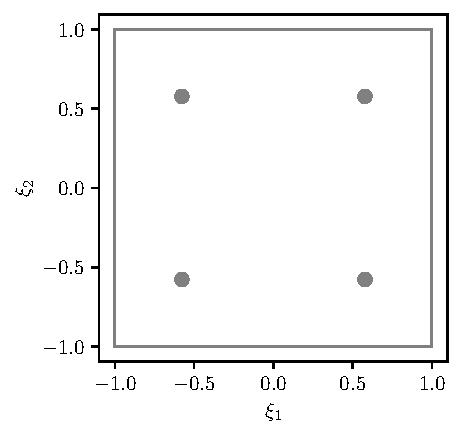
\includegraphics[width=0.5\textwidth]{figures/reference_element.pdf}
    \end{center}

    In this local coordinate system, we can interpolate any variable defined on nodes $\mathbf{a}_j$ by an approximation
    \begin{equation}
        a = \mathbf{N}(\pmb{\xi}) \cdot  \mathbf{a}_j
    \end{equation}
    with shape functions $\mathbf{N}(\pmb{\xi})$ interpolating the values at the four element nodes
    \begin{equation}
        \mathbf{a}_j = 
        \begin{pmatrix}
            a_j^0\\ 
            a_j^1\\ 
            a_j^2\\ 
            a_j^3\\
        \end{pmatrix}.
    \end{equation}
    For a quadrilateral linear reference element, the shape functions are given by 
    \begin{equation}
        \mathbf{N}(\pmb{\xi}) = \frac{1}{4}
        \begin{pmatrix}
            (1-\xi_1)(1-\xi_2) \\
            (1+\xi_1)(1-\xi_2) \\
            (1+\xi_1)(1+\xi_2) \\
            (1-\xi_1)(1+\xi_2)
        \end{pmatrix}
    \end{equation}
    such that each function assumes the value 1 at one node of the element and the value 0 at all other nodes of the element. The four shape functions $N_1, N_2, N_3, N_4$ of the linear quadrilateral reference element are displayed in the following figure for $\Omega_j = [-1,1]^2$.
    

    \begin{center}
        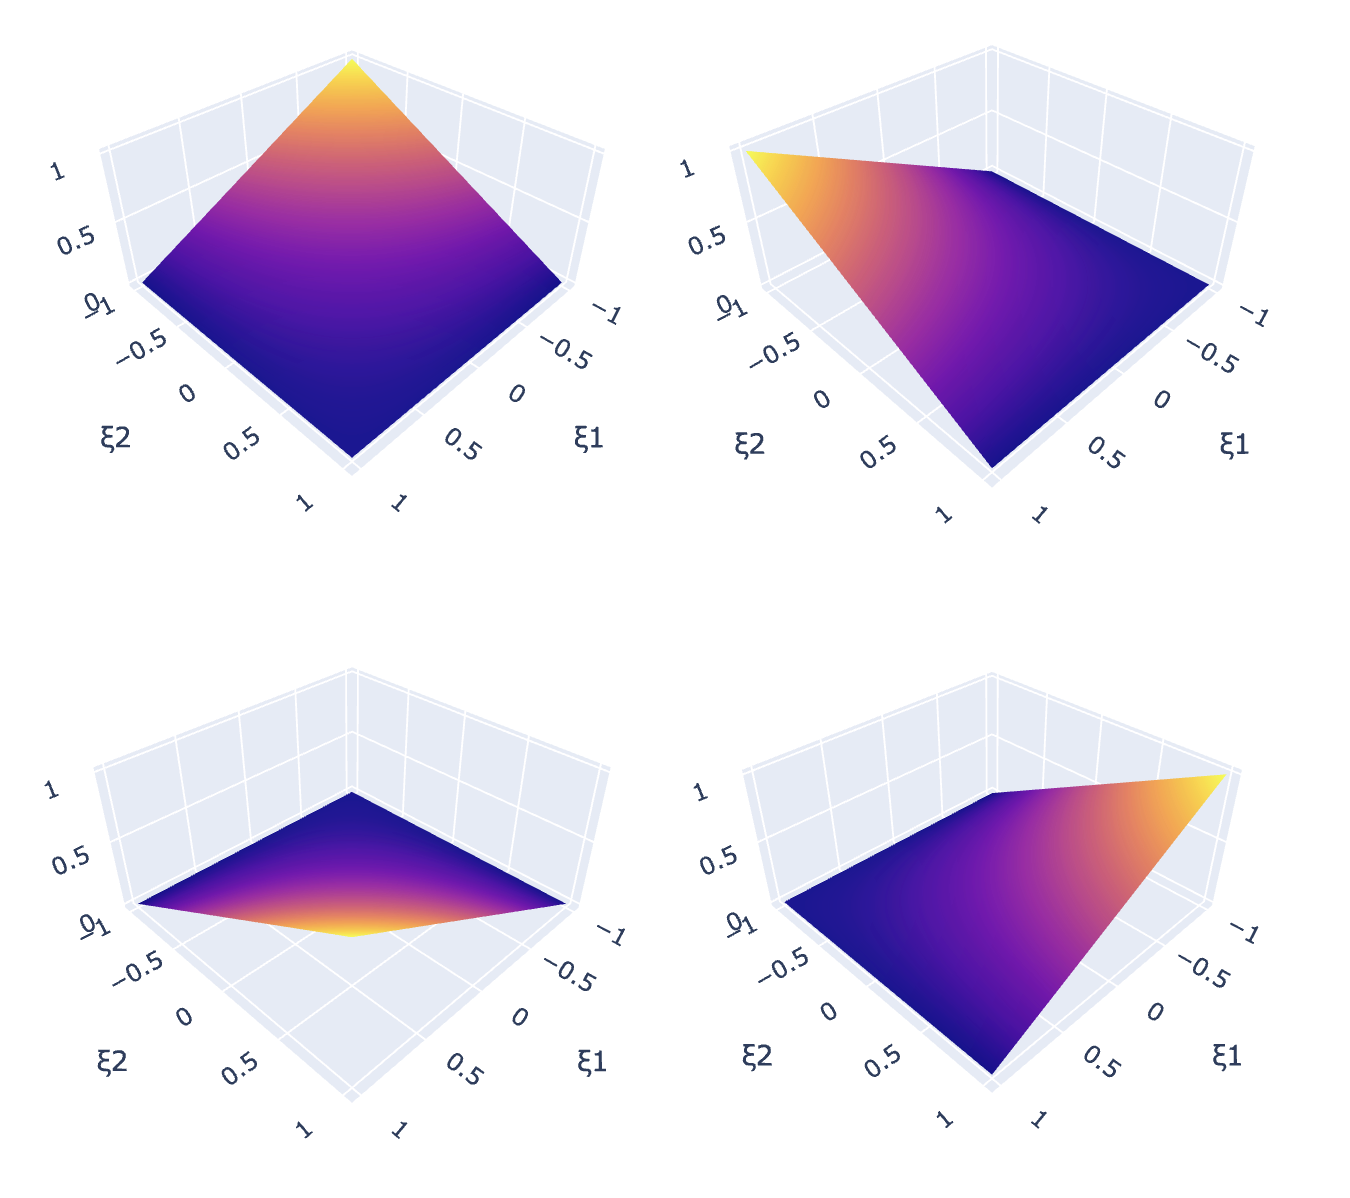
\includegraphics[width=0.7\textwidth]{figures/quad_shape_functions.png}
    \end{center}

    The shape functions enable us to compute gradients on each reference element as 
    \begin{equation}
        \nabla_\xi a = \mathbf{B}_\textrm{ref}(\pmb{\xi}) \cdot  \mathbf{a}_j
    \end{equation}
    with 
    \begin{equation}
        \mathbf{B}^\textrm{ref}(\pmb{\xi})
        =  \nabla_\xi \mathbf{N}(\pmb{\xi}) 
        = 
        \begin{pmatrix}
            \frac{\partial \mathbf{N}(\pmb{\xi})}{\partial \xi_1} \\ 
            \frac{\partial \mathbf{N}(\pmb{\xi})}{\partial \xi_2} 
        \end{pmatrix} 
        = \frac{1}{4}
        \begin{pmatrix}
            -1 + \xi_2 & 1 - \xi_2 & 1 + \xi_2 & -1 - \xi_2 \\
            -1 + \xi_1 & -1 - \xi_1 & 1 + \xi_1 & 1 - \xi_1
        \end{pmatrix}
    \end{equation}

    These gradients are formulated w.r.t. the reference system $\xi_1, \xi_2$. Employing the chain rule, we may formulate gradients w.r.t. to the global coordinates as 
    \begin{equation}
        \nabla a = 
        \underbrace{
        \begin{pmatrix}
            \frac{\partial \xi_1}{\partial x_1} & \frac{\partial \xi_2}{\partial x_1} \\
            \frac{\partial \xi_1}{\partial x_2} & \frac{\partial \xi_2}{\partial x_2} \\
        \end{pmatrix}
        }_\textrm{Chain rule}
        \cdot 
        \mathbf{B}^\textrm{ref}(\pmb{\xi}) \cdot  \mathbf{a}_j
    \end{equation}

    We may use the shape functions $\mathbf{N}(\pmb{\xi})$ to interpolate the nodal positions of an element $j$ by 
    \begin{equation}
        x_1(\pmb{\xi})
        = 
        \mathbf{N}(\pmb{\xi})
        \cdot 
        \begin{pmatrix}
            {(x_1)}_j^0 \\
            {(x_1)}_j^1 \\
            {(x_1)}_j^2 \\
            {(x_1)}_j^3 \\
        \end{pmatrix}
        , \quad
        x_2(\pmb{\xi})
        = 
        \mathbf{N}(\pmb{\xi})
        \cdot 
        \begin{pmatrix}
            {(x_2)}_j^0 \\
            {(x_2)}_j^1 \\
            {(x_2)}_j^2 \\
            {(x_2)}_j^3 \\
        \end{pmatrix}
    \end{equation}
    or use $\mathbf{B}^\textrm{ref}(\pmb{\xi})$ to compute the gradients
    \begin{equation}
        \begin{pmatrix}
            \frac{\partial x_1}{\partial \xi_1} \\
            \frac{\partial x_1}{\partial \xi_2}\\
        \end{pmatrix}
        = 
        \mathbf{B}^\textrm{ref}(\pmb{\xi})
        \cdot 
        \begin{pmatrix}
            {(x_1)}_j^0 \\
            {(x_1)}_j^1 \\
            {(x_1)}_j^2 \\
            {(x_1)}_j^3 \\
        \end{pmatrix}
        , \quad
        \begin{pmatrix}
            \frac{\partial x_2}{\partial \xi_1} \\
            \frac{\partial x_2}{\partial \xi_2}\\
        \end{pmatrix}
        = 
        \mathbf{B}^\textrm{ref}(\pmb{\xi})
        \cdot 
        \begin{pmatrix}
            {(x_2)}_j^0 \\
            {(x_2)}_j^1 \\
            {(x_2)}_j^2 \\
            {(x_2)}_j^3 \\
        \end{pmatrix}.
    \end{equation}
    The latter gradients can be used to compute the \emph{Jacobian} 
    \begin{equation}
        \mathbf{J}_j(\pmb{\xi})
        = 
        \begin{pmatrix}
            \frac{\partial x_1}{\partial \xi_1} & \frac{\partial x_2}{\partial \xi_1} \\
            \frac{\partial x_1}{\partial \xi_2} & \frac{\partial x_2}{\partial \xi_2}
        \end{pmatrix},
    \end{equation}
    which is just the inverse of the missing term of the chain rule. Hence we can determine the interpolated gradient of $a$ w.r.t. the global coordinate system as 
    \begin{equation}
        \nabla a = 
        \underbrace{
            \mathbf{J}_j^{-1}(\pmb{\xi}) 
            \cdot 
            \mathbf{B}^\textrm{ref}(\pmb{\xi})
            }_{\mathbf{B}(\pmb{\xi})}
        \cdot  \mathbf{a}_j
    \end{equation}
\end{example}

\begin{example}{Gauss–Legendre quadrature}{quadratureexample} 
    In addition to the interpolation, we need to find numerical solutions to the integral. Hence, this is a quick recap of the Gauss-legendre quadrature. 
    
    Consider an integral in $\mathcal{R}$
    \begin{equation}
        \int_{a}^{b} f(x) dx.
    \end{equation}
    We can solve this by transforming it to a unit domain
    \begin{equation}
        \int_{-1}^{1} f(\xi) \frac{\text{d}x}{\text{d}\xi} \text{d}\xi
    \end{equation}
    with 
    \begin{equation}
        \frac{dx}{d\xi} = \frac{b-a}{2}.
    \end{equation}
    For this unit domain, we can express the integral as a summation with tabulated positions $\xi^k$ and weights $w^k$ like
    \begin{equation}
        \int_{-1}^{1} f(\xi) \frac{\text{d}x}{\text{d}\xi} \text{d}\xi
        = \sum_{k=1}^m w^k f(\xi^k) \frac{\text{d}x}{\text{d}\xi} \xi.
    \end{equation}
    This summation via Gauss quadrature is able to integrate polynomials up to an order $2m-1$ exactly. For example, using two points ($m=2$) with 
    \begin{equation}
        \xi^1 = -\frac{1}{\sqrt{3}}, \quad \xi^2 = \frac{1}{\sqrt{3}}
    \end{equation}
    and weights $w^1=1$ and $w^2=1$ enables exact integration of polynomials up to order 3, which is sufficient for our integrals as we approximate the integral functions with linear shape functions. 

    \begin{center}
        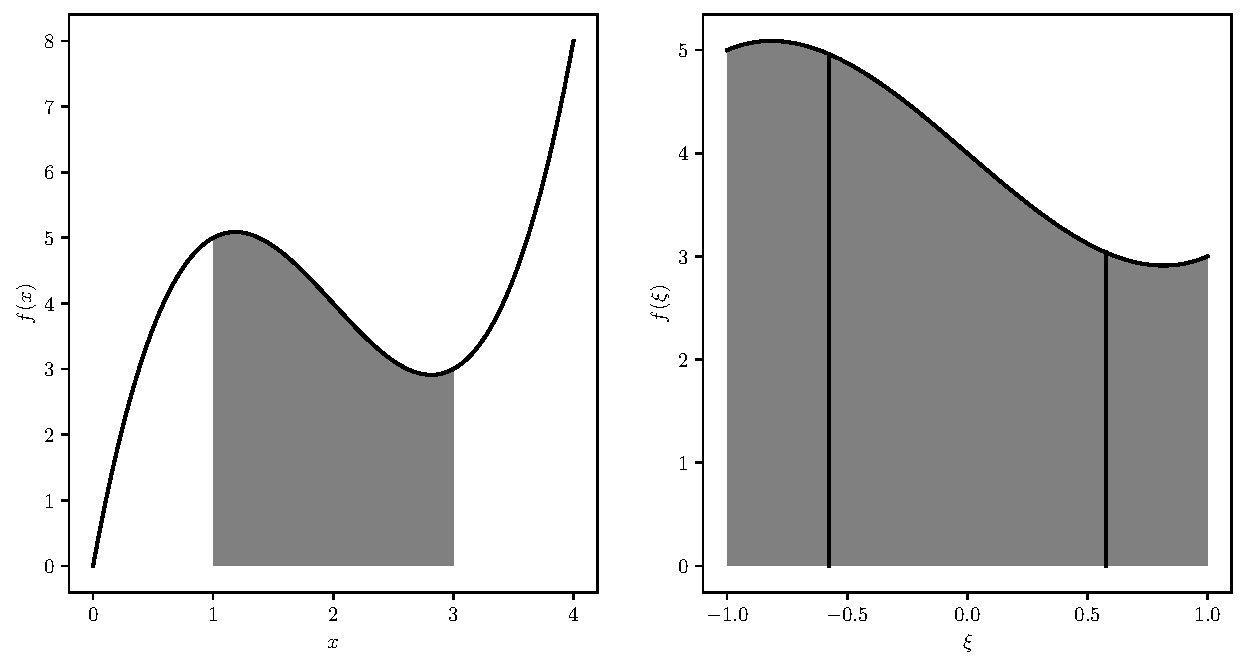
\includegraphics[width=\textwidth]{figures/gauss_legendre.pdf}
    \end{center}
    
    This one-dimensional example can be extended canonically to higher dimensions by replacing $\frac{\text{d}x}{\text{d}\xi}$ with the determinant of the Jacobian and by using positions 
    \begin{equation}
        \pmb{\xi}^1 = \begin{pmatrix}-\frac{1}{\sqrt{3}} \\ -\frac{1}{\sqrt{3}}\end{pmatrix} 
        \quad
        \pmb{\xi}^2 = \begin{pmatrix}-\frac{1}{\sqrt{3}} \\ \frac{1}{\sqrt{3}}\end{pmatrix} 
        \quad
        \pmb{\xi}^3 = \begin{pmatrix}\frac{1}{\sqrt{3}} \\ -\frac{1}{\sqrt{3}}\end{pmatrix} 
        \quad
        \pmb{\xi}^4 = \begin{pmatrix}\frac{1}{\sqrt{3}} \\ \frac{1}{\sqrt{3}}\end{pmatrix} 
        \label{eq:gaussian_weights}
    \end{equation}
    which are indicated as gray points in the sketch of the reference element in the previous example.
\end{example}

In conclusion, the definition of shape functions on an element allows us to interpolate nodal properties (like position, displacements or temperatures) and to compute gradients of these properties within the element. In addition, Gauss-Legendre quadrature allows us to integrate these properties over the element domain and thus to evaluate the integrals in Equation \eqref{eq:discretized_weak_form}. The following subsection addresses this procedure for each of the terms in Equation \eqref{eq:discretized_weak_form}.

\subsection{External work by body forces}
Let's start with the body force term and transform the integral from the original domain to the reference element as
\begin{equation}
    \int_{\Omega_j} \mathbf{b} \cdot \mathbf{v} \text{d}A
    = 
    \int_{\Omega_j^\textrm{ref}} \mathbf{b} \cdot \mathbf{v}(\pmb{\xi})
    \hspace{0.25em} \text{det}\left(\mathbf{J}_j(\pmb{\xi})\right)\text{d}A^\textrm{ref}
\end{equation}
using the determinant of the Jacobian as a scaling factor between $\text{d}A$ and $\text{d}A^\textrm{ref}$. This scaling is equivalent to the usage of $\frac{\text{d}x}{\text{d}\xi}$ in the one-dimensional example. 

We can then use Gauss–Legendre quadrature with two positions per dimension to perform a numerical integration of this term as
\begin{equation}
    \int_{\Omega_j^\textrm{ref}} \mathbf{b} \cdot \mathbf{v}(\pmb{\xi}) \hspace{0.25em}\text{det}\left(\mathbf{J}_j(\pmb{\xi})\right)\text{d}A^\textrm{ref}
    = \sum_{k=1}^4 w^k \text{det}\left(\mathbf{J}_j(\pmb{\xi}^k)\right) \mathbf{b} \cdot \mathbf{v}(\pmb{\xi}^k).
\end{equation}
Essentially, this turns the integral into a weighted sum of function values at specific positions $\pmb{\xi}^k$. In this case, we chose $w^k=1$ and positions according to Equation \eqref{eq:gaussian_weights}.
Using the shape functions, we may then express the last variable using the nodal values of the trial function $\mathbf{v}_j$ as  
\begin{equation}
    \mathbf{v}(\pmb{\xi}^k) 
    =
    \begingroup 
    \setlength\arraycolsep{-5pt}
    \begin{pmatrix}
            N_1(\pmb{\xi}^k) & 0 & N_2(\pmb{\xi}^k) & 0 & N_3(\pmb{\xi}^k) & 0 & N_4(\pmb{\xi}^k) & 0\\
            0 & N_1(\pmb{\xi}^k) & 0 & N_2(\pmb{\xi}^k) & 0 & N_3(\pmb{\xi}^k) & 0 & N_4(\pmb{\xi})\\
    \end{pmatrix} 
    \endgroup
    \cdot 
    \begin{pmatrix}
            {(v_1)}_j^0 \\
            {(v_2)}_j^0 \\
            {(v_1)}_j^1 \\
            {(v_2)}_j^1 \\
            {(v_1)}_j^2 \\
            {(v_2)}_j^2 \\
            {(v_1)}_j^3 \\
            {(v_2)}_j^3 
    \end{pmatrix}.
    \label{eq:shape_interpolation}
\end{equation}
In summary, we transformed the body force term of a single element from 
\begin{equation}
    \int_{\Omega_j} \mathbf{b} \cdot \mathbf{v} \text{d}A  
\end{equation}
to a scalar vector product 
\begin{equation}
    \underbrace{\sum_k \text{det}\left(\mathbf{J}_j(\pmb{\xi}^k)\right) \mathbf{b} \cdot \begingroup 
    \setlength\arraycolsep{-5pt}
    \begin{pmatrix}
            N_1(\pmb{\xi}^k) & 0 & N_2(\pmb{\xi}^k) & 0 & N_3(\pmb{\xi}^k) & 0 & N_4(\pmb{\xi}^k) & 0\\
            0 & N_1(\pmb{\xi}^k) & 0 & N_2(\pmb{\xi}^k) & 0 & N_3(\pmb{\xi}^k) & 0 & N_4(\pmb{\xi})\\
    \end{pmatrix} 
    \endgroup}_{\mathbf{f}^\Omega_j}
    \cdot 
    \mathbf{v}_j
\end{equation}
where $\mathbf{f}^\Omega_j \in \mathcal{R}^8$ describes the nodal body forces on element $j$. 

\subsection{Strain energy term}
Similar to the body force term, we can evaluate the strain energy term of an element in Equation \eqref{eq:discretized_weak_form} by transforming the integral and applying Gauss-Legendre quadrature as 
\begin{equation}
    \int_{\Omega_j} \mathbf{E}(\mathbf{u}) : \mathbb{C} :  \mathbf{E}(\mathbf{v}) \text{d}A 
    = \sum_k \mathbf{E}\left(\mathbf{u}(\pmb{\xi^k})\right) : \mathbb{C} :  \mathbf{E}\left(\mathbf{v}(\pmb{\xi^k})\right)  \text{det}\left(\mathbf{J}_j(\pmb{\xi}^k)\right).
\end{equation}
The double contraction is unnecessarily complex for a two-dimensional problem and we can simplify it as follows:
\begin{equation}
    \mathbf{E}\left(\mathbf{u}(\pmb{\xi^k})\right) : \mathbb{C} :  \mathbf{E}\left(\mathbf{v}(\pmb{\xi^k})\right) = 
    \pmb{\varepsilon}\left(\mathbf{u}(\pmb{\xi}^k)\right)
    \cdot 
    \mathbf{C}
    \cdot 
    \pmb{\varepsilon}\left(\mathbf{v}(\pmb{\xi}^k)\right)
\end{equation}
with a two-dimensional stiffness matrix
\begin{align}
        \mathbf{C} &= \begin{pmatrix}
        2G+\Lambda & \Lambda & 0 \\
        \Lambda & 2G+\Lambda &  0 \\
        0 & 0 & G \\
    \end{pmatrix} \textrm{(isotropic plane strain)}\\
    \mathbf{C} &= \frac{E}{1-\nu^2}\begin{pmatrix}
        1 & \nu & 0 \\
        \nu & 1 &  0 \\
        0 & 0 & (1-\nu)/2 \\
    \end{pmatrix} \textrm{(isotropic plane stress)}
\end{align}
and with two-dimensional strains
\begin{equation}
    \pmb{\varepsilon}(\mathbf{u}) = 
    \begin{pmatrix}
        \frac{\partial u_1}{\partial x_1} \\ 
        \frac{\partial u_2}{\partial x_2} \\
        \frac{\partial u_1}{\partial x_2} + \frac{\partial u_2}{\partial x_1}\\
    \end{pmatrix}
    \quad 
    \textrm{and}
    \quad
    \pmb{\varepsilon}(\mathbf{v}) = 
    \begin{pmatrix}
        \frac{\partial v_1}{\partial x_1} \\ 
        \frac{\partial v_2}{\partial x_2} \\
        \frac{\partial v_1}{\partial x_2} + \frac{\partial v_2}{\partial x_1}\\
    \end{pmatrix}.
\end{equation}
We can express the strain terms with shape functions as 
\begin{equation}
    \pmb{\varepsilon}\left(\mathbf{v}\right)
    =
    \underbrace{
    \begingroup 
    \setlength\arraycolsep{2pt}
    \begin{pmatrix}
            B_{11}(\pmb{\xi}^k) & 0 & B_{12}(\pmb{\xi}^k) & 0 & B_{13}(\pmb{\xi}^k) & 0 & B_{14}(\pmb{\xi}^k) & 0\\
            0 & B_{21}(\pmb{\xi}^k) & 0 & B_{22}(\pmb{\xi}^k) & 0 & B_{23}(\pmb{\xi}^k) & 0 & B_{24}(\pmb{\xi}^k)\\
            B_{21}(\pmb{\xi}^k) & B_{11}(\pmb{\xi}^k) & B_{22}(\pmb{\xi}^k) & B_{12}(\pmb{\xi}^k) & B_{23}(\pmb{\xi}^k) & B_{13}(\pmb{\xi}^k) & B_{24}(\pmb{\xi}^k) & B_{14}(\pmb{\xi}^k)\\
    \end{pmatrix} 
    \endgroup
    }_{\mathbf{D}}
    \cdot 
    \mathbf{v}_j
\end{equation}
for the derivatives of the trial function and analogous for the displacements. In conclusion, we can transform the integral 
\begin{equation}
    d_j \int_{\Omega_j} \mathbf{E}(\mathbf{u}) : \mathbb{C} :  \mathbf{E}(\mathbf{v}) \text{d}A 
\end{equation}
to a matrix vector product 
\begin{equation}
    \mathbf{u}_j \cdot 
    \underbrace{
    d_j 
    \underbrace{ 
    \sum_k \text{det}\left(\mathbf{J}_j(\pmb{\xi}^k)\right)\mathbf{D}^\top \cdot \mathbf{C} \cdot \mathbf{D}}_{\mathbf{k}^0_j}
    }_{\mathbf{k}_j}
    \cdot \mathbf{v}_j
\end{equation}
with an element stiffness matrix $\mathbf{k}_j = d_j  \mathbf{k}^0_j \in \mathcal{R}^{8x8}$. 

\subsection{External work by boundary traction}
Finally, the boundary traction term in Equation \eqref{eq:discretized_weak_form} is treated in a similar fashion to the previous terms. However, the boundary of a two-dimensional domain is just a line and we integrate it with two points along the element edge as 
\begin{equation}
    \int_{\partial \Omega_{N,j}} \mathbf{t} \cdot \mathbf{v} \text{d}s
    =
    \sum_k \mathbf{t}(\xi^k) \cdot \mathbf{v}(\xi^k) \frac{\partial x}{\partial \xi} 
\end{equation}

Using Equation \eqref{eq:shape_interpolation}, we may denote this as 
\begin{equation}
    \underbrace{\sum_k \frac{\partial x}{\partial \xi} \mathbf{t}(\pmb{\xi}^k) \cdot \begingroup 
    \setlength\arraycolsep{-5pt}
    \begin{pmatrix}
            N_1(\pmb{\xi}^k) & 0 & N_2(\pmb{\xi}^k) & 0 & N_3(\pmb{\xi}^k) & 0 & N_4(\pmb{\xi}^k) & 0\\
            0 & N_1(\pmb{\xi}^k) & 0 & N_2(\pmb{\xi}^k) & 0 & N_3(\pmb{\xi}^k) & 0 & N_4(\pmb{\xi})\\
    \end{pmatrix} 
    \endgroup}_{\mathbf{f}^\Gamma_j}
    \cdot 
    \mathbf{v}_j
\end{equation}
where $\mathbf{f}^\Gamma_j \in \mathcal{R}^8$ describes the nodal traction forces on element $j$. 

\section{Assembly of linear systems of equations}

At this point, we can transform Equation \eqref{eq:discretized_weak_form} to 
\begin{equation}
    \sum_{j=0}^{M-1} \mathbf{f}^\Gamma_j \cdot \mathbf{v}_j
    - \sum_{j=0}^{M-1} \mathbf{u}_j \cdot \mathbf{k}_j \cdot \mathbf{v}_j
    + \sum_{j=0}^{M-1} \mathbf{f}^\Omega_j \cdot \mathbf{v}_j = 0 \quad \forall \mathbf{v}_j.
\end{equation}
with element-wise matrices that are very similar to the truss system from Chapter 5. Rearranging this equation yields 
\begin{equation}
    \sum_{j=0}^{M-1} \mathbf{v}_j \cdot \left( \mathbf{f}^\Gamma_j + \mathbf{f}^\Omega_j \right)
    = \sum_{j=0}^{M-1} \mathbf{v}_j \cdot \mathbf{k}_j \cdot \mathbf{u}_j \quad \forall \mathbf{v}_j.
\end{equation}
We can assemble this sum of linear equation systems to a global equation system 
\begin{equation}
    \mathbf{v} \cdot \mathbf{f} = \mathbf{v} \cdot \mathbf{K} \cdot \mathbf{u}
\end{equation}
with 
\begin{equation}
    \mathbf{v} = 
    \begin{pmatrix}
    \begin{smallmatrix}
        \dots \\ (v_1)^0_j \\ (v_2)^0_j \\ \dots \\ (v_1)^1_j \\ (v_2)^1_j \\ \dots \\ (v_1)^2_j \\ (v_2)^2_j \\ \dots \\ (v_1)^3_j \\ (v_2)^3_j \\ \dots \\
    \end{smallmatrix}
    \end{pmatrix}
    \quad
    \text{and}
    \quad
    \mathbf{u}
    \begin{pmatrix}
    \begin{smallmatrix}
        \dots \\ (u_1)^0_j \\ (u_2)^0_j \\ \dots \\ (u_1)^1_j \\ (u_2)^1_j \\ \dots \\
        \dots \\ (u_1)^2_j \\ (u_2)^2_j \\ \dots \\ (u_1)^3_j \\ (u_2)^3_j \\ \dots
    \end{smallmatrix}
    \end{pmatrix}
    \quad
    \text{and}
    \quad
    \mathbf{f} = 
    \sum_j
    \begin{pmatrix}
    \begin{smallmatrix}
        \dots \\ (f^\Gamma_1)^0_j + (f^\Omega_1)^0_j \\ (f^\Gamma_2)^0_j + (f^\Omega_2)^0_j \\ \dots \\ (f^\Gamma_1)^1_j + (f^\Omega_1)^1_j \\ (f^\Gamma_2)^1_j + (f^\Omega_2)^1_j\\ \dots \\ (f^\Gamma_1)^2_j + (f^\Omega_1)^2_j \\ (f^\Gamma_2)^2_j + (f^\Omega_2)^2_j \\ \dots \\ (f^\Gamma_1)^3_j + (f^\Omega_1)^3_j \\ (f^\Gamma_2)^3_j + (f^\Omega_2)^3_j \\ \dots \\
    \end{smallmatrix}
    \end{pmatrix}.
\end{equation}
and
\begin{equation}
    \mathbf{K} =
    \sum_j
    \underbrace{
    \begin{pmatrix}
    \begin{smallmatrix}
    \dots & \dots & \dots & \dots & \dots & \dots & \dots & \dots & \dots & \dots & \dots & \dots & \dots \\
    \dots & (k_{11})_j & (k_{12})_j & \dots & (k_{13})_j & (k_{14})_j & \dots & (k_{15})_j & (k_{16})_j & \dots & (k_{17})_j & (k_{18})_j & \dots  \\
     \dots & (k_{21})_j & (k_{22})_j & \dots & (k_{23})_j & (k_{24})_j & \dots & (k_{25})_j & (k_{26})_j & \dots & (k_{27})_j & (k_{28})_j & \dots  \\
    \dots & \dots & \dots & \dots & \dots & \dots & \dots  \\
    \dots & (k_{31})_j & (k_{32})_j & \dots & (k_{33})_j & (k_{34})_j & \dots & (k_{35})_j & (k_{36})_j & \dots & (k_{37})_j & (k_{38})_j & \dots  \\
    \dots & (k_{41})_j & (k_{42})_j & \dots & (k_{43})_j & (k_{44})_j & \dots & (k_{45})_j & (k_{46})_j & \dots & (k_{47})_j & (k_{48})_j & \dots  \\
    \dots & \dots & \dots & \dots & \dots & \dots & \dots  \\
    \dots & (k_{51})_j & (k_{52})_j & \dots & (k_{53})_j & (k_{54})_j & \dots & (k_{55})_j & (k_{56})_j & \dots & (k_{57})_j & (k_{58})_j & \dots  \\
     \dots & (k_{61})_j & (k_{62})_j & \dots & (k_{63})_j & (k_{64})_j & \dots & (k_{65})_j & (k_{66})_j & \dots & (k_{67})_j & (k_{68})_j & \dots  \\
    \dots & \dots & \dots & \dots & \dots & \dots & \dots  \\
    \dots & (k_{71})_j & (k_{72})_j & \dots & (k_{73})_j & (k_{74})_j & \dots & (k_{75})_j & (k_{76})_j & \dots & (k_{77})_j & (k_{78})_j & \dots  \\
    \dots & (k_{81})_j & (k_{82})_j & \dots & (k_{83})_j & (k_{84})_j & \dots & (k_{85})_j & (k_{86})_j & \dots & (k_{87})_j & (k_{88})_j & \dots  \\
    \dots & \dots & \dots & \dots & \dots & \dots & \dots  \\
    \end{smallmatrix}
    \end{pmatrix}
    }_{\mathbf{K}_j}
\end{equation}
where the 64 entries of the element stiffness are placed at corresponding positions for the global degrees of freedom in a global stiffness tensor $\mathbf{K}$. Assuming $\mathbf{u}_0=\mathbf{0}$ and using the fact that the test function $\mathbf{v}$ is arbitrary (but zero on the essential boundary) we end up with a reduced system 
\begin{equation}
     \mathbf{f}_\textrm{red} = \mathbf{K}_\textrm{red} \cdot \mathbf{u}_\textrm{red} 
     \label{eq:reduced_system_fem}
\end{equation}
just like previously with the truss system in Chapter 5. Now it comes down to solving this linear system of equations in order to compute the solution $\mathbf{u}_\textrm{red}$.

\begin{example}{Finite element solution of a cantilever beam}{femexample} 
    The following example shows a simple 2D cantilever beam discretized with 722 nodes and 666 linear quad elements. This results in 1444 degrees of freedom in total. The cantilever beam is subjected to a point load at the tip and clamped at one side. There is no body force acting on it ($\mathbf{b} = \mathbf{0}$).
    \begin{center}
        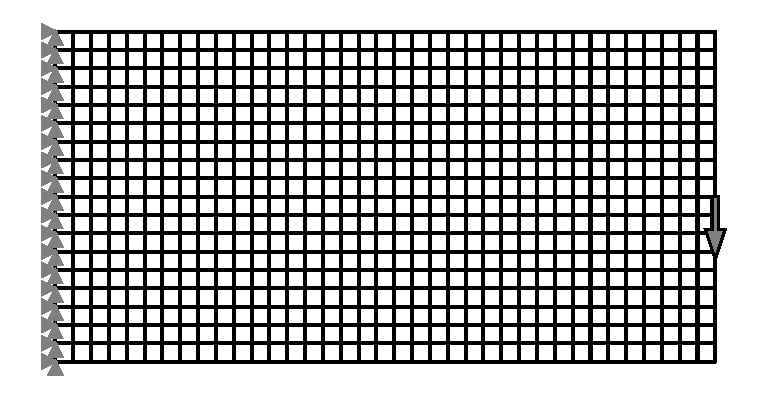
\includegraphics[width=0.8\textwidth]{figures/cantilever_fem.pdf}
    \end{center}
    Evaluation of the integrals and assembling it leads to a global system 
    \begin{equation}
        \mathbf{f} = \mathbf{K} \mathbf{u}
    \end{equation}
    with $\mathbf{f}, \mathbf{u} \in \mathcal{R}^{1444}$ and $\mathbf{K} \in \mathcal{R}^{1444x1444}$. Elimination of the 38 constrained degrees of freedom results in 
    \begin{equation}
        \mathbf{f}_\textrm{red} = \mathbf{K}_\textrm{red} \mathbf{u}_\textrm{red}
    \end{equation}
    with $\mathbf{f}_\textrm{red}, \mathbf{u}_\textrm{red} \in \mathcal{R}^{1406}$ and $\mathbf{K}_\textrm{red} \in \mathcal{R}^{1406x1406}$. This can be solved for $\mathbf{u}_\textrm{red}$ representing the displacements at each node. The subsequent figure shows the norm of the displacement interpolated with linear shape functions.
    \begin{center}
        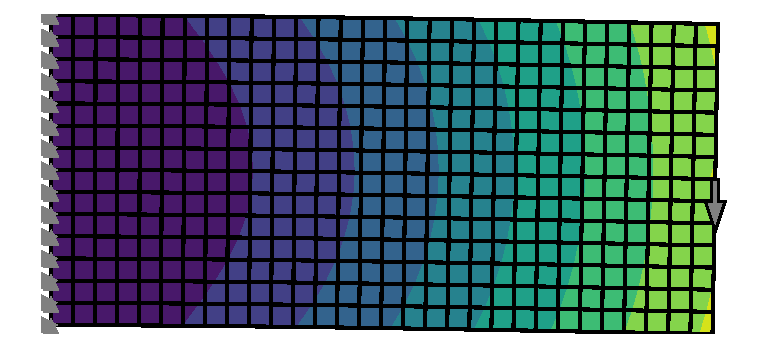
\includegraphics[width=0.8\textwidth]{figures/cantilever_fem_solved.pdf}
    \end{center}
\end{example}

\bibliographystyle{unsrtnat}
\bibliography{literature} 




\chapter{Topology optimization in continua}
In the previous chapter, we learned how to transform a continuous elastic problem on a two-dimensional domain into a discrete problem using finite elements. 

\begin{objectives}{}{objectives_topology}
After studying this chapter and finishing the exercise, you should be able to 
\begin{itemize}[label=$\dots$]
    \item transfer solution methods from sizing problems to FEM-discretized problems
    \item solve for binary topologies using the SIMP approach
    \item discuss numerical problems in topology optimization
    \item apply filters to deal with numerical problems and manufacturing constraints
\end{itemize}
\end{objectives}

\section{Variable thickness sheet problem}
\label{sec:variable_thickness_sheet}
Let's consider a two-dimensional domain discretized with finite elements, in which we can adjust the thickness of each element. We may seek the best distribution of thicknesses $\mathbf{d}$ to minimize compliance $C$ with a constrained amount of material volume $V_0$. This problem can be formulated in analogy to the standard problem of sizing optimization stated in Equation \eqref{eq:size_optimization}: 

\begin{equation}
    \begin{aligned}
        \min_{\mathbf{d}} \quad & C(\mathbf{d}) = \mathbf{f} \cdot \mathbf{u}(\mathbf{d})\\
        \textrm{s.t.} \quad & \mathbf{d} \cdot \mathbf{A} - V_0 \le 0  \\
                            & \mathbf{d} \in \mathcal{D}\\
    \end{aligned}
    \label{eq:sheet_optimization}
\end{equation}

Mathematically, this problem is equivalent to the truss problem and can be solved in the same way: We formulate the Lagrangian
\begin{equation}
    \mathcal{L}(\mathbf{d}, \mu) = C(\mathbf{d}) + \mu \left( \mathbf{d} \cdot \mathbf{A} - V_0 \right) 
    \label{eq:lagrangian_sheet_optimization}
\end{equation}
and determine its derivative
\begin{equation}
    \frac{\partial \mathcal{L} (\mathbf{d}, \mu)}{\partial d_j} 
    = \frac{\partial C(\mathbf{d})}{\partial d_j} + \mu A_j 
\end{equation}
with 
\begin{equation}
    \frac{\partial C}{\partial d_j} = -2w_j(\mathbf{d}) = - \mathbf{u}_j(\mathbf{d})  \cdot \mathbf{k}^0_j \cdot \mathbf{u}_j(\mathbf{d}).
    \label{eq:sensitivity_sheet}
\end{equation}
In comparison to Equation \eqref{eq:compliance_sensitivity} for trusses with four degrees of freedom, the element displacement vector contains eight degrees of freedom for these 2D problems with linear quad elements ($\mathbf{u}_j \in \mathcal{R}^8, \mathbf{k}^0_j \in \mathcal{R}^{8\times 8}$). 

Just like the truss problem, the variable thickness sheet problem can be approximated using MMA with lower asymptotes only. Subsequently, it is solved with the dual method and a line search to find the Lagrange parameter $\mu$. The entire procedure is identical to Section \ref{sec:truss_topology}, if we replace the truss cross sections $\mathbf{a}$ with element thicknesses $\mathbf{d}$ and the truss lengths $\mathbf{l}$ with element areas $\mathbf{A}$.

\begin{example}{Cantilever beam with MMA}{cantileveroptimizationexample}
    Consider a FEM cantilever beam from the previous example. Instead of just computing the displacements, we are now interested in finding the optimal thickness of each element given a volume constraint.

    We formulate the following algorithm to solve that problem: 
    \begin{enumerate}
        \item Define the cantilever FEM model with all nodes $\mathcal{N}$, elements $\mathcal{E}$, material property $E$, volume constraint $V_0$, design limits $\mathbf{d}^l, \mathbf{d}^u$ and the initial design choice $\mathbf{d}^0$.
        \item Compute the displacements $\mathbf{u}^k = \mathbf{u}(\mathbf{d}^k)$ by solving the FEM system for the current design $\mathbf{d}^k$.
        \item Compute the strain energies per area for all elements using the previously computed displacements   
        \begin{equation}
            w^k_j(\mathbf{d}^k) = \frac{1}{2}\mathbf{u}^k_j  \cdot \mathbf{k}^0_j \cdot \mathbf{u}^k_j
        \end{equation}
        \item Compute the lower asymptotes as $\mathbf{L}^k =\mathbf{d}^k - s (\mathbf{d}^u - \mathbf{d}^l)$ with $s \in (0,1)$ during the first two iterations and according to 
        \begin{equation}
            L^k_j = 
            \begin{cases}
                d^k_j - s  (d^{k-1}_j-L^{k-1}_j) & (d_j^k-d_j^{k-1})(d_j^{k-1}-d_j^{k-2}) < 0\\
                d^k_j - \frac{1}{\sqrt{s}}  (d^{k-1}_j-L^{k-1}_j) & \text{else}
            \end{cases}
        \end{equation}
        in the following iterations.
        \item Compute the lower move limit as 
        \begin{equation}
            \tilde{\mathbf{d}}^{l,k} = \max(\mathbf{d}_l,  0.9 \mathbf{L}^k + 0.1 \mathbf{d}^k)
        \end{equation}
        \item Evaluate the analytical solution
            \begin{align}
                \hat{d}_j(\mu) &= L_j^k + \sqrt{\frac{2 w_j (\mathbf{d}^k)
                (L^k_j-d^k_j)^2}{\mu A_j}} \\
                \mathbf{d}^* (\mu) &= \max\left(\tilde{\mathbf{d}}^{l,k}, \min \left(\hat{\mathbf{d}}(\mu), \mathbf{d}_u \right)\right)
            \end{align}
        \item Perform a line search to find the root $\mu^*>0$ in 
        \begin{equation}
            \frac{\partial \underline{\mathcal{L}}}{\partial \mu}(\mu) = \mathbf{A} \cdot \mathbf{d}^* (\mu) - V_0  = 0
        \end{equation}
        with Newton's method or bisection method. 
        \item Repeat with steps 2-7 until convergence or a maximum number of iterations is reached.
    \end{enumerate}

    The following image shows a result of the algorithm for the cantilever problem stated above. Black areas use the full maximum thickness $\mathbf{d}^u$ and white areas use the minimum thickness $\mathbf{d}^l$. The intermediate values are represented by different shades of gray.

    \begin{center}
        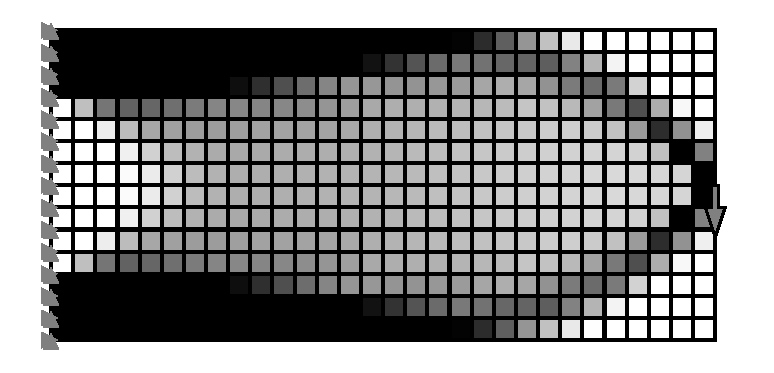
\includegraphics[width=\linewidth]{figures/cantilever_fem_optimized.pdf}
    \end{center}
    
\end{example}

\section{Solid isotropic material with penalization (SIMP)}
\label{sec:simp}
The problem stated in Equation \eqref{eq:sheet_optimization} is essentially a sizing optimization problem. In a topology optimization, we seek a material distribution, where each element is either completely filled or completely unfilled with material. We can formulate such a problem by reinterpreting the thickness variable as a normalized material density $\pmb{\rho}$, where $\rho_j=1$ indicates presence of material and $\rho_j=0$ indicates absence of material in element $j$. The stiffness of each element becomes a function of $\rho_j$, e.g. 
\begin{equation}
    \mathbb{C}(\rho_j)=
    \begin{cases}
        \mathbb{C} & \text{if} \quad \rho_j = 1 \\
        0          & \text{if} \quad \rho_j = 0
    \end{cases}
\end{equation}

Then, the problem statement reads
\begin{equation}
    \begin{aligned}
        \min_{\pmb{\rho}} \quad & C(\pmb{\rho}) = \mathbf{f} \cdot \mathbf{u}(\pmb{\rho})\\
        \textrm{s.t.} \quad & \pmb{\rho} \cdot \mathbf{V} - V_0 \le 0  \\
                            & \rho_j \in \{0, 1\}\\
    \end{aligned}
    \label{eq:topology_optimization}
\end{equation}

where the only change compared to Equation \eqref{eq:sheet_optimization} is the discrete nature of the design variables $\pmb{\rho}$ and the name of the design variables. Hence, we formulate the Lagrangian analogously to Equation \eqref{eq:lagrangian_sheet_optimization} as 
\begin{equation}
    \mathcal{L}(\pmb{\rho}, \mu) = C(\pmb{\rho}) + \mu \left( \pmb{\rho} \cdot \mathbf{A} - V_0 \right).
    \label{eq:lagrangian_topology_optimization}
\end{equation}

Unfortunately, the binary problem is notoriously hard to solve, because we cannot compute gradients on the solution and testing all solutions is computationally inaccessible. Hence we try to formulate a continuous relation between stiffness and normalized density that still results in a binary result. One such formulation is called \emph{Solid Isotropic Material with Penalization} (SIMP) and denoted as 
\begin{equation}
    \mathbb{C}(\rho_j)= \rho_j^p \mathbb{C}
\end{equation}
with a penalization parameter $p \ge 1$. 
The effect of penalization is shown in Figure \ref{fig:simp} for typical values of $p$. We may observe for $p>1$ that the stiffness per invested material is unattractive for intermediate density values. For example, choosing $\rho_j=0.5$ adds half an element volume to the total volume, but contributes only a quarter of the stiffness compared to a fully filled element. An optimization that tries to minimize compliance for a given volume will therefore rather favor elements that provide the full stiffness benefit ($\rho=1$) or do not count towards the constraint ($\rho=\rho^l$). 

\begin{figure}[!htpb]
    \centering
    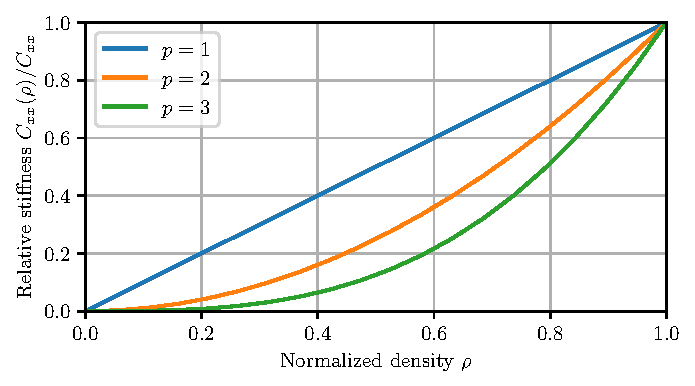
\includegraphics[width=0.9\textwidth]{figures/simp.pdf}
    \caption{Penalization factors in SIMP.}
    \label{fig:simp}
\end{figure}

Incorporating the SIMP method to the optimization is straight-forward. We just need to adjust the sensitivity (see Equation \ref{eq:sensitivity_sheet}) slightly to
\begin{equation}
    \frac{\partial C}{\partial \rho_j} = -2 p \rho_j^{p-1} w_j(\pmb{\rho}^k) = - p \rho_j^{p-1} \mathbf{u}_j(\pmb{\rho})  \cdot \mathbf{k}^0_j \cdot \mathbf{u}_j(\pmb{\rho}).
    \label{eq:sensitivity_topology}
\end{equation}

\begin{example}{Cantilever beam with MMA and SIMP}{cantileversimpoptimizationexample}
    Consider a FEM cantilever beam from the previous example. We only adjust the solution in Step 6 towards 
    \begin{equation}
        \hat{\rho}_j(\mu) = L_j^k + \sqrt{\frac{-2p \rho_j^{p-1} w_j(\pmb{\rho}^k)
        (L^k_j-d^k_j)^2}{\mu A_j}}
    \end{equation}
    and we end up with the following solution:
    \begin{center}
        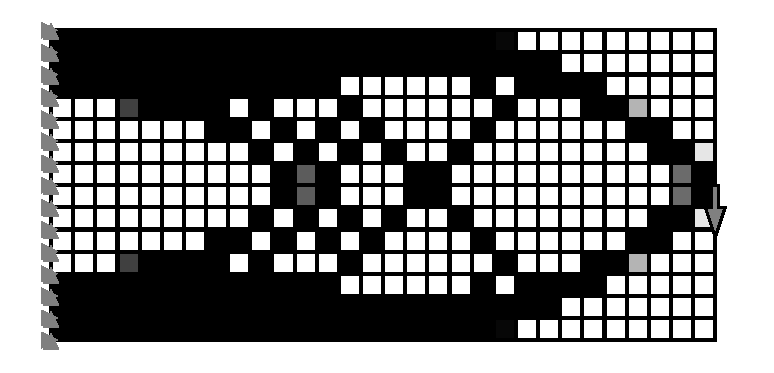
\includegraphics[width=\linewidth]{figures/cantilever_fem_optimized_binary.pdf}
    \end{center}
\end{example}

\section{Filters}
Obviously, the SIMP approach helps us to find a binary solution of the discretized problem stated in Equation \eqref{eq:topology_optimization}. However, we may ask ourselves if there is a unique solution to this problem independent of discretization. And it turns out, the answer is no: You can improve any given design by replacing it with finer structures in a process that goes on indefinitely \cite{Christensen2008}. 
In addition to the theoretical non-existence of a solution, this also means that our solution is \emph{mesh-dependent}: If we want to refine the solution, we may end up with a totally different solution. 

\begin{example}{Cantilever beam mesh dependency}{cantileverdiscoptimizationexample}
    We can increase the resolution of the previous examples to achieve better compliance results. However, this demonstrates the mesh-dependence of the solution and we observe structures which might be difficult to manufacture.
    
    Finer resolution:
    \begin{center}
        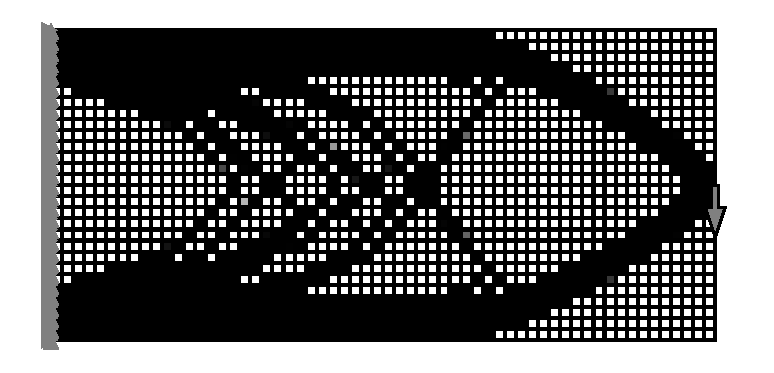
\includegraphics[width=\linewidth]{figures/cantilever_fem_optimized_binary_fine.pdf}
    \end{center}
    
    Even finer resolution:
    \begin{center}
        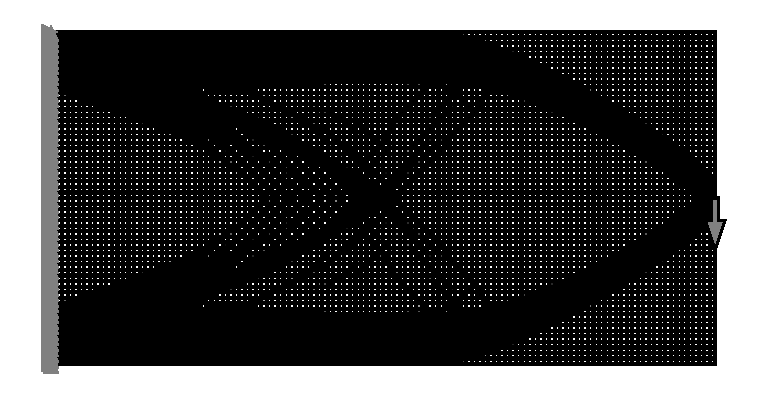
\includegraphics[width=\linewidth]{figures/cantilever_fem_optimized_binary_extra_fine.pdf}
    \end{center}
\end{example}

Even if we were to accept mesh dependence and the theoretical problems, we are still left with challenges in the resulting designs. First of all, fine structures may be hard to manufacture. Even additive manufacturing methods are limited to some minimal structure size. Secondly, we may observe checkerboard-like patterns on the structure. These are numerical artifacts from the fact that we use linear shape functions which lead to an overestimation of the stiffness for that configuration.

We can address all these problems with the introduction of filters as a regularization \cite{Harzheim2014, Lazarov2011}. There are two traditional approaches for mesh-independent filtering: \emph{density filtering} and \emph{sensitivity filtering}. In density filtering, we replace the density $\pmb{\rho}$ with a weighted sum of neighboring densities, and use this filtered density $\tilde{\pmb{\rho}}$ in the stiffness evaluation
\begin{equation}
    \mathbb{C}(\rho_j)= \tilde{\rho}_j^p(\pmb{\rho}) \mathbb{C}.
\end{equation}
The filtered density is computed according to 
\begin{equation}
    \tilde{\rho}_j (\pmb{\rho}) = \frac{\sum_i H_{ji} A_i \rho_i}{\sum_i H_{ji} A_i}
\end{equation}
with a distance weighting matrix
\begin{equation}
    H_{ji} = 
    \begin{cases}
        R-\lVert \mathbf{x}_i - \mathbf{x}_j\rVert & \text{if} \quad \lVert \mathbf{x}_i - \mathbf{x}_j\rVert \le R \\
        0 & \text{else},
    \end{cases}
\end{equation}
where $R$ describes the filter radius. This filter results in a structural weakening of structures finer than $R$, as they get smeared with neighboring empty elements. Hence, the filter solves the mesh-dependency problem, prevents structures that cannot be manufactured and prevents checkerboard patterns. However, we need to account for the filter during sensitivity computation by 
\begin{equation}
    \frac{\partial C}{\partial \rho_j} 
    = \frac{\partial C}{\partial \tilde{\rho}_m} \frac{\partial \tilde{\rho}_m}{\partial \rho_j}
    = \frac{\partial C}{\partial \tilde{\rho}_m}  \frac{H_{jm} A_m }{\sum_i H_{ji} A_i}
\end{equation}
and in the volume constraint.

An alternative to filtering densities is filtering of sensitivities. We may compute the filtered sensitivity as
\begin{equation}
    \widetilde{\frac{\partial C}{\partial \rho_j}} = \frac{1}{\rho_j} \frac{\sum_i H_{ji} A_i \rho_i \frac{\partial C}{\partial \rho_i} }{\sum_i H_{ji} A_i}
\end{equation}
which is a purely heuristic concept, i.e. there is no mathematical proof for this filter to work \cite{Sigmund1998}. However, we can implement this formulation simply by replacing the sensitivities in \eqref{eq:sensitivity_topology} with filtered sensitivities. This is very efficient, simple to implement and experience shows that this filter works quite well.

\begin{example}{Cantilever beam  with sensitivity filtering}{cantileverfilterexample}
    The following images show the optimized cantilever beams from previous examples with enabled sensitivity filtering. Filtering prevents small structures and regularizes the problem such that we achieve similar optimal designs for different mesh sizes.

    Previous example:
    \begin{center}
        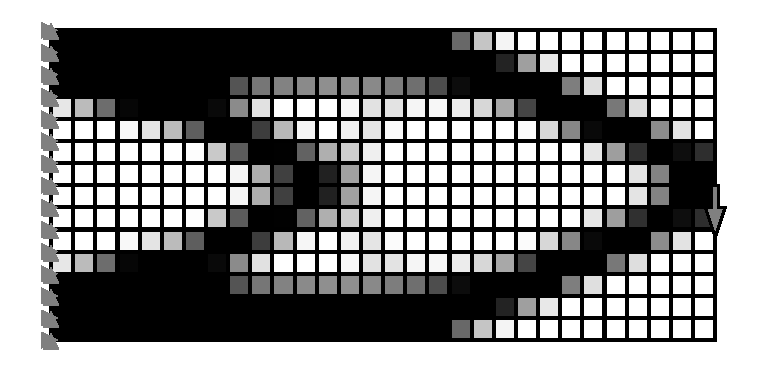
\includegraphics[width=\linewidth]{figures/cantilever_fem_optimized_binary_filtered.pdf}
    \end{center}
    
    Finer resolution:
    \begin{center}
        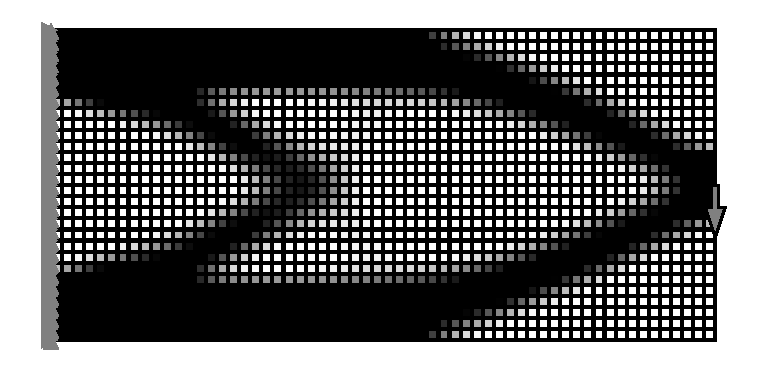
\includegraphics[width=\linewidth]{figures/cantilever_fem_optimized_binary_fine_filtered.pdf}
    \end{center}
    
    Even finer resolution:
    \begin{center}
        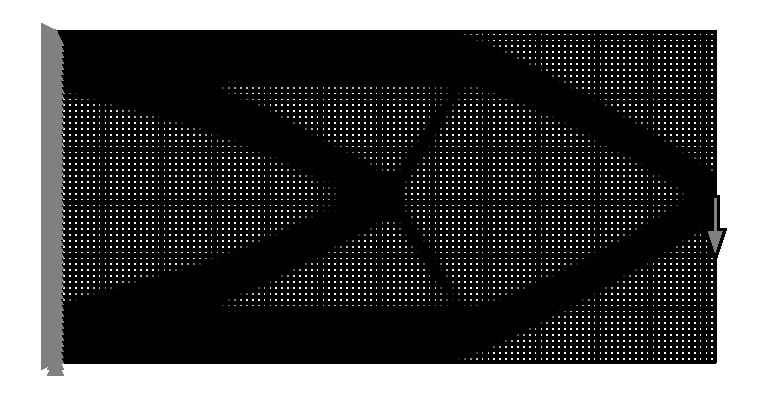
\includegraphics[width=\linewidth]{figures/cantilever_fem_optimized_binary_extra_fine_filtered.pdf}
    \end{center}
\end{example}

There is one more challenge in the SIMP formulation of the standard topology optimization problem: For $p>1$, the problem is not convex anymore and different starting points may result in different local minima \cite{Christensen2008}. A strategy to cure termination at non-global minima is a gradual increase of $p$ starting from $p=1$ and using multiple starting points $\pmb{\rho}^0$.

\section{Optimality criteria}
The solution via MMA is in line with the previous chapters of this manuscript and is able to solve arbitrary problems beyond the compliance minimization stated in problem \eqref{eq:topology_optimization}. Historically, this specific problem was first solved with the \emph{optimality criteria method} instead of convex approximations. The idea here is that we can use the gradient of the Lagrangian given in Equation \eqref{eq:lagrangian_topology_optimization}
\begin{equation}
    \frac{\partial \mathcal{L} (\pmb{\rho}, \mu)}{\partial\rho_j} 
    = \frac{\partial C(\pmb{\rho})}{\partial \rho_j} + \mu A_j = 0
\end{equation}
to formulate an optimality condition
\begin{equation}
    G_j = \frac{-\frac{\partial C(\pmb{\rho})}{\partial \rho_j}}{\mu A_j} = \frac{p \rho_j^{p-1} \mathbf{u}_j(\pmb{\rho})  \cdot \mathbf{k}^0_j \cdot \mathbf{u}_j(\pmb{\rho})}{\mu A_j} = 1
\end{equation}
that must be fulfilled at the optimum whenever a variable does not reach its bounds.
A heuristic algorithm can now compute $G_j$ and adjust $\rho_j$ such that $G_j$ approaches 1. We may realize that increasing $\rho_j^k$ increases the stiffness and hence decreases the displacement for a given load. Consequently, increasing $\rho_j$ decreases $G_j$ and vice versa. Hence, an update rule 
\begin{equation}
    \hat{\rho}_j^{k+1} = \left(G_j^k\right)^\xi \rho_j^k 
\end{equation}
drives the solution towards the optimal point $\rho_j^*$, where $G^*_j=1$. The exponent $\xi \in (0,1]$ stabilizes the algorithm with typical values being $\xi=0.5$ \cite{Harzheim2014}. 

In addition, we employ move limits 
\begin{align}
    \rho_j^{l,k} &= \max \left(\rho_j^l, (1-m)\rho_j^k \right) \\
    \rho_j^{u,k} &= \min \left(\rho_j^u, (1+m)\rho_j^k \right)
\end{align}
to compute the next value as 
\begin{equation}
    \rho_j^{k+1} = \max \left( \min \left(\hat{\rho}_j^{k+1}, \rho_j^{u,k} \right), \rho_j^{l,k} \right).
\end{equation}
The move limits reduce the maximum step width and account for bounds on the design variables. 

To compute $G_j$, we need to determine the value of the Lagrange multiplier $\mu$. For the compliance problem, we can intuitively assume that the stiffest structure will use all material and consequently, that the volume constraint will be active. the Lagrange multiplier may be found with the bisection method on the feasibility condition
\begin{equation}
    \frac{\partial \mathcal{L}}{\partial \mu} = \pmb{\rho}(\mu) \cdot \mathbf{A} - V_0 = 0.
\end{equation}

\begin{example}{Algorithm with optimality criteria and SIMP}{ocexample}
    Consider a FEM cantilever beam from the previous example. 

    We formulate the following algorithm to solve that problem: 
    \begin{enumerate}
        \item Define the cantilever FEM model with all nodes $\mathcal{N}$, elements $\mathcal{E}$, material property $E$, volume constraint $V_0$, design limits $\mathbf{d}^l, \mathbf{d}^u$ and the initial design choice $\mathbf{d}^0$.
        \item Compute the displacements $\mathbf{u}^k = \mathbf{u}(\mathbf{d}^k)$ by solving the FEM system for the current design $\mathbf{d}^k$.
        \item Apply the bisection method to find the root of 
            \begin{equation}
                g(\mu) = \pmb{\rho}^{k+1}(\mu) \cdot \mathbf{A} - V_0
            \end{equation}
        with 
        \begin{equation}
            \pmb{\rho}^{k+1}(\mu) = \max \left( \min \left(\left(G_j^k(\mu)\right)^\xi \rho_j^k , \rho_j^{u,k} \right), \rho_j^{l,k} \right).
        \end{equation}
        \item Repeat with steps 2-3 until convergence or a maximum number of iterations is reached.
    \end{enumerate}
\end{example}

In addition to the density-based method shown so far, topology optimization may also be performed with \emph{Level-Set methods} and empirical growth rules like \emph{Soft Kill Option}. These methods are not addressed in this lecture.

\section{Interpretation}
Finally, it is important to note that topology optimizations provide only design suggestions and not a design than can be readily manufactured. With the current state of research, we always need to interpret the result in the context of a manufacturing method.

\begin{example}{Cantilever beam  interpretation}{cantileverinterpretationexample}
    We may project the solution of a topology optimization problem to a canvas in a CAD software and use it as a guide to sketch an actual component:
    \begin{center}
        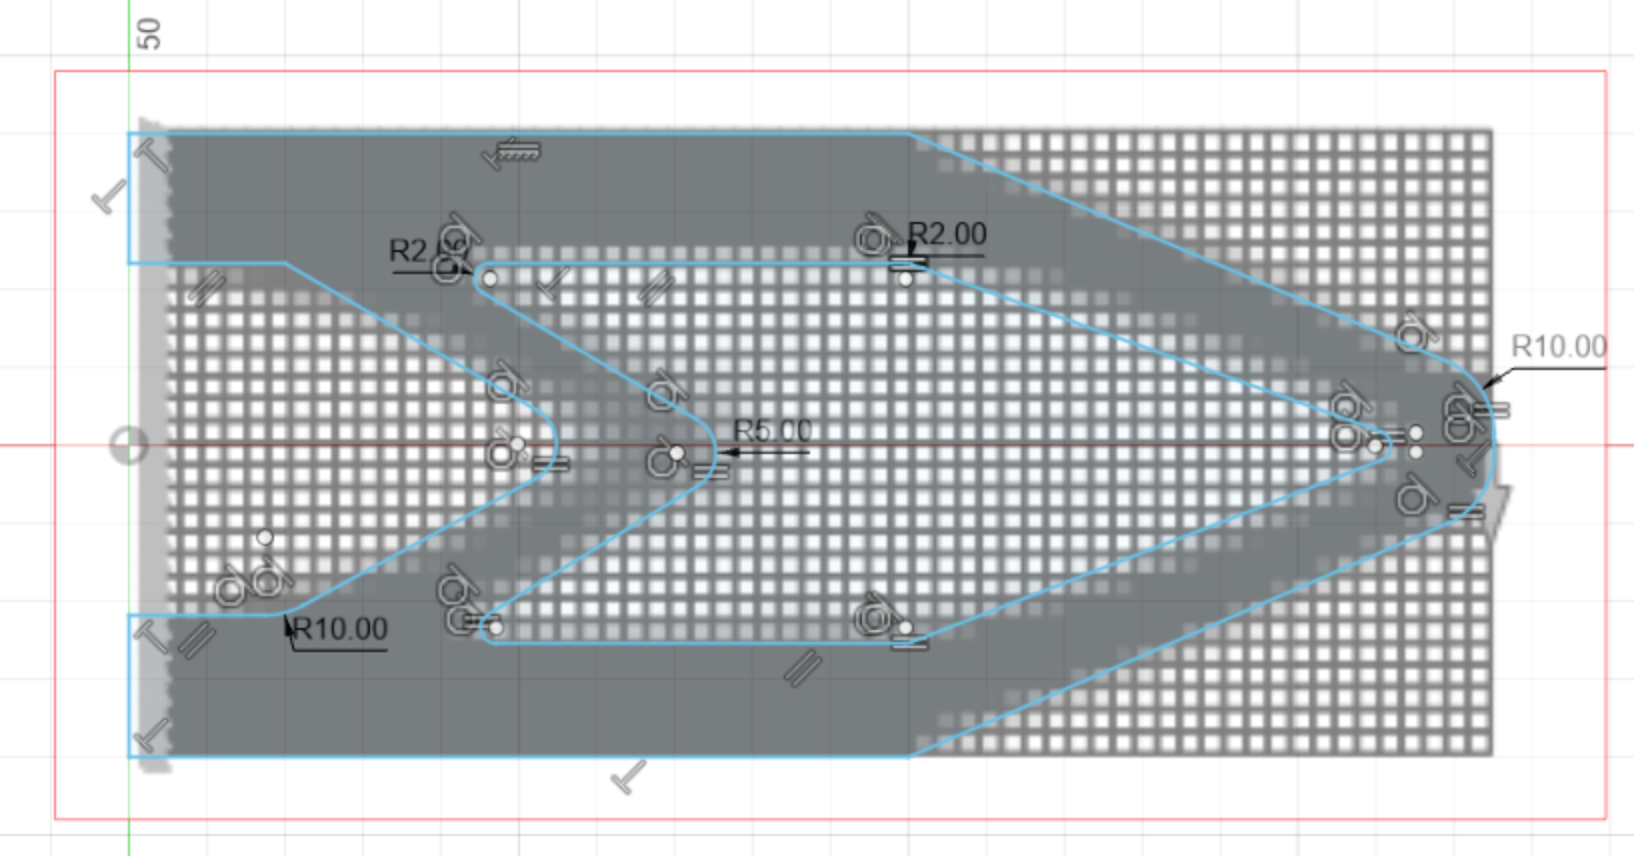
\includegraphics[width=\linewidth]{figures/cantilever_template.png}
    \end{center}
    
    This is an interpretation of the cantilever beam as a sheet metal design:
    \begin{center}
        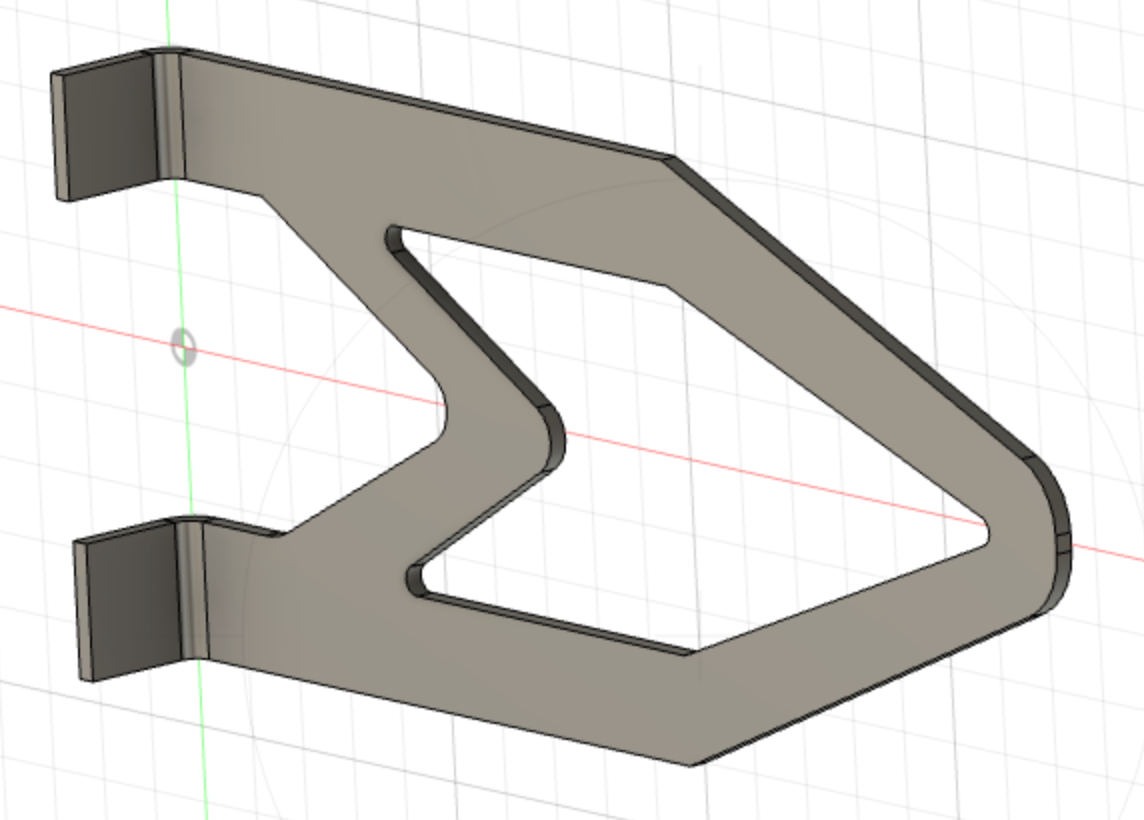
\includegraphics[width=\linewidth]{figures/cantilever_design.png}
    \end{center}
\end{example}


\bibliographystyle{unsrtnat}
\bibliography{literature} 


\end{document}
